\chapter{Implementación}

En este capítulo se detalla la implementación de la plataforma desarrollada, describiendo las decisiones técnicas, herramientas y metodologías empleadas para materializar los objetivos planteados. La arquitectura del sistema se fundamenta en la separación clara entre el backend, responsable del procesamiento de datos y la lógica principal de la aplicación, y el frontend, encargado de la presentación e interacción con el usuario. Esta aproximación modular facilita el mantenimiento, escalabilidad y futuras extensiones del sistema. 

\begin{figure}[H]
  \centering
  \fbox{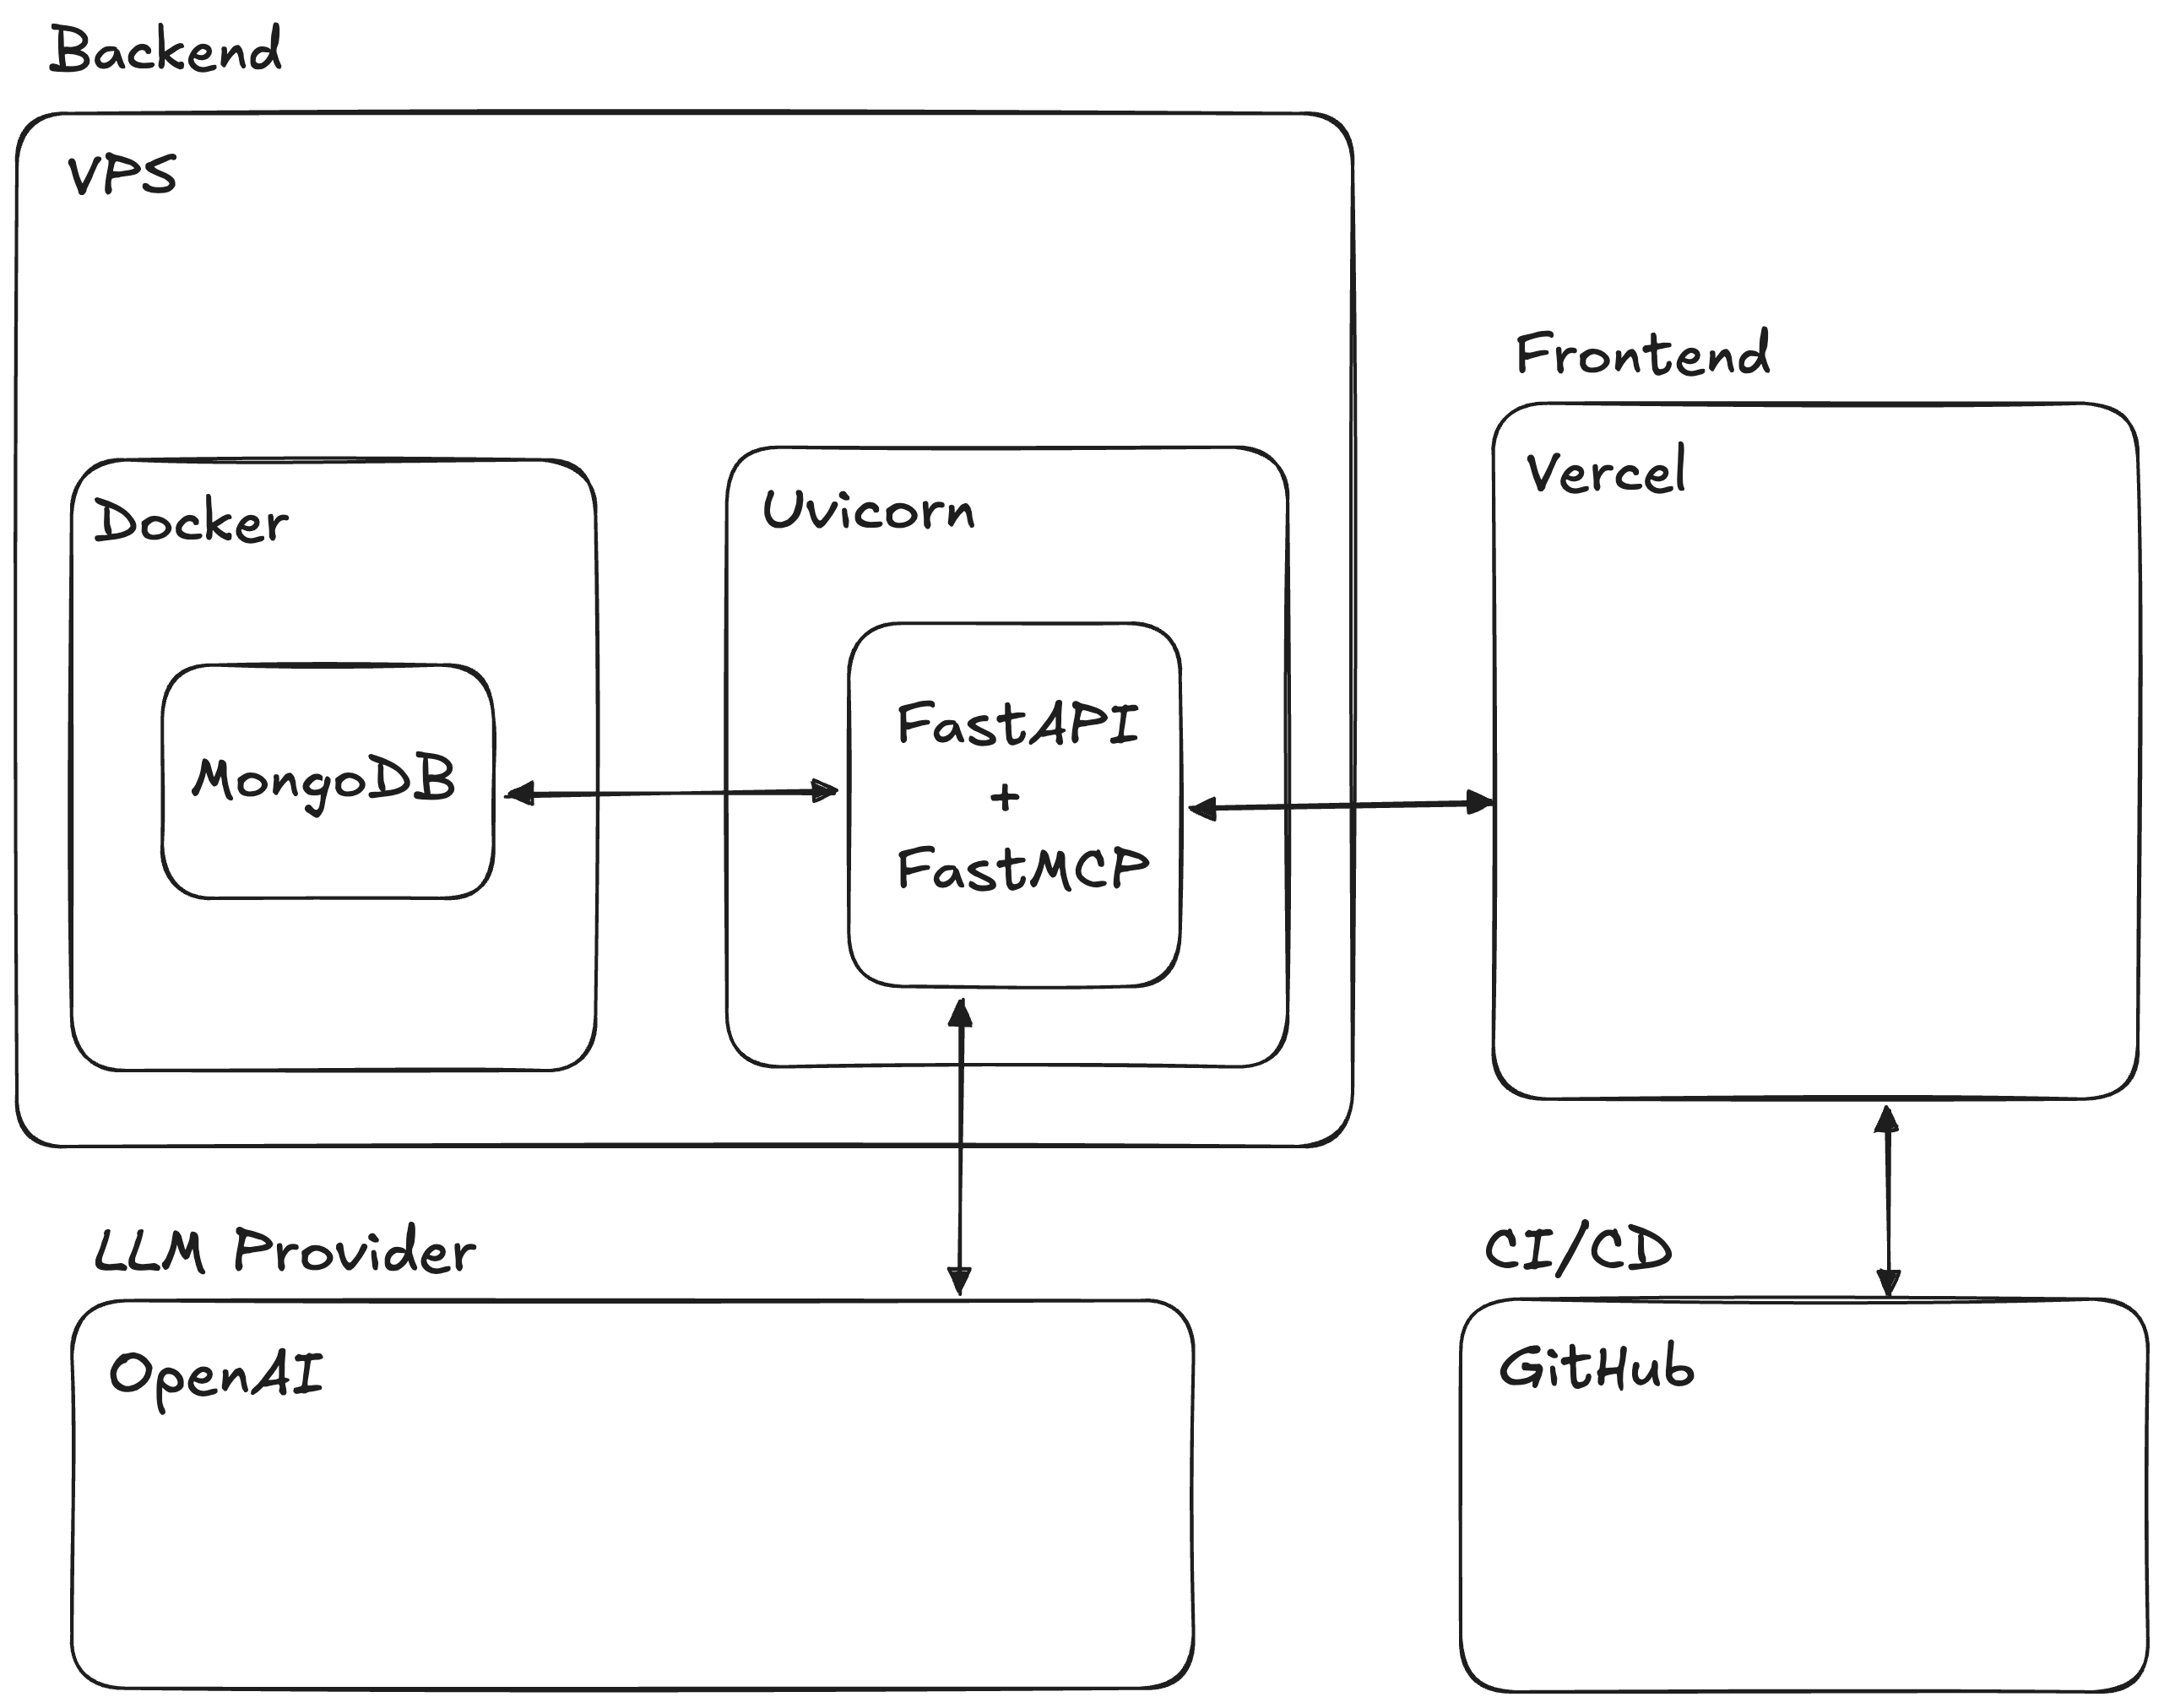
\includegraphics[width=0.9\textwidth]{imagenes/arch1.png}}
  %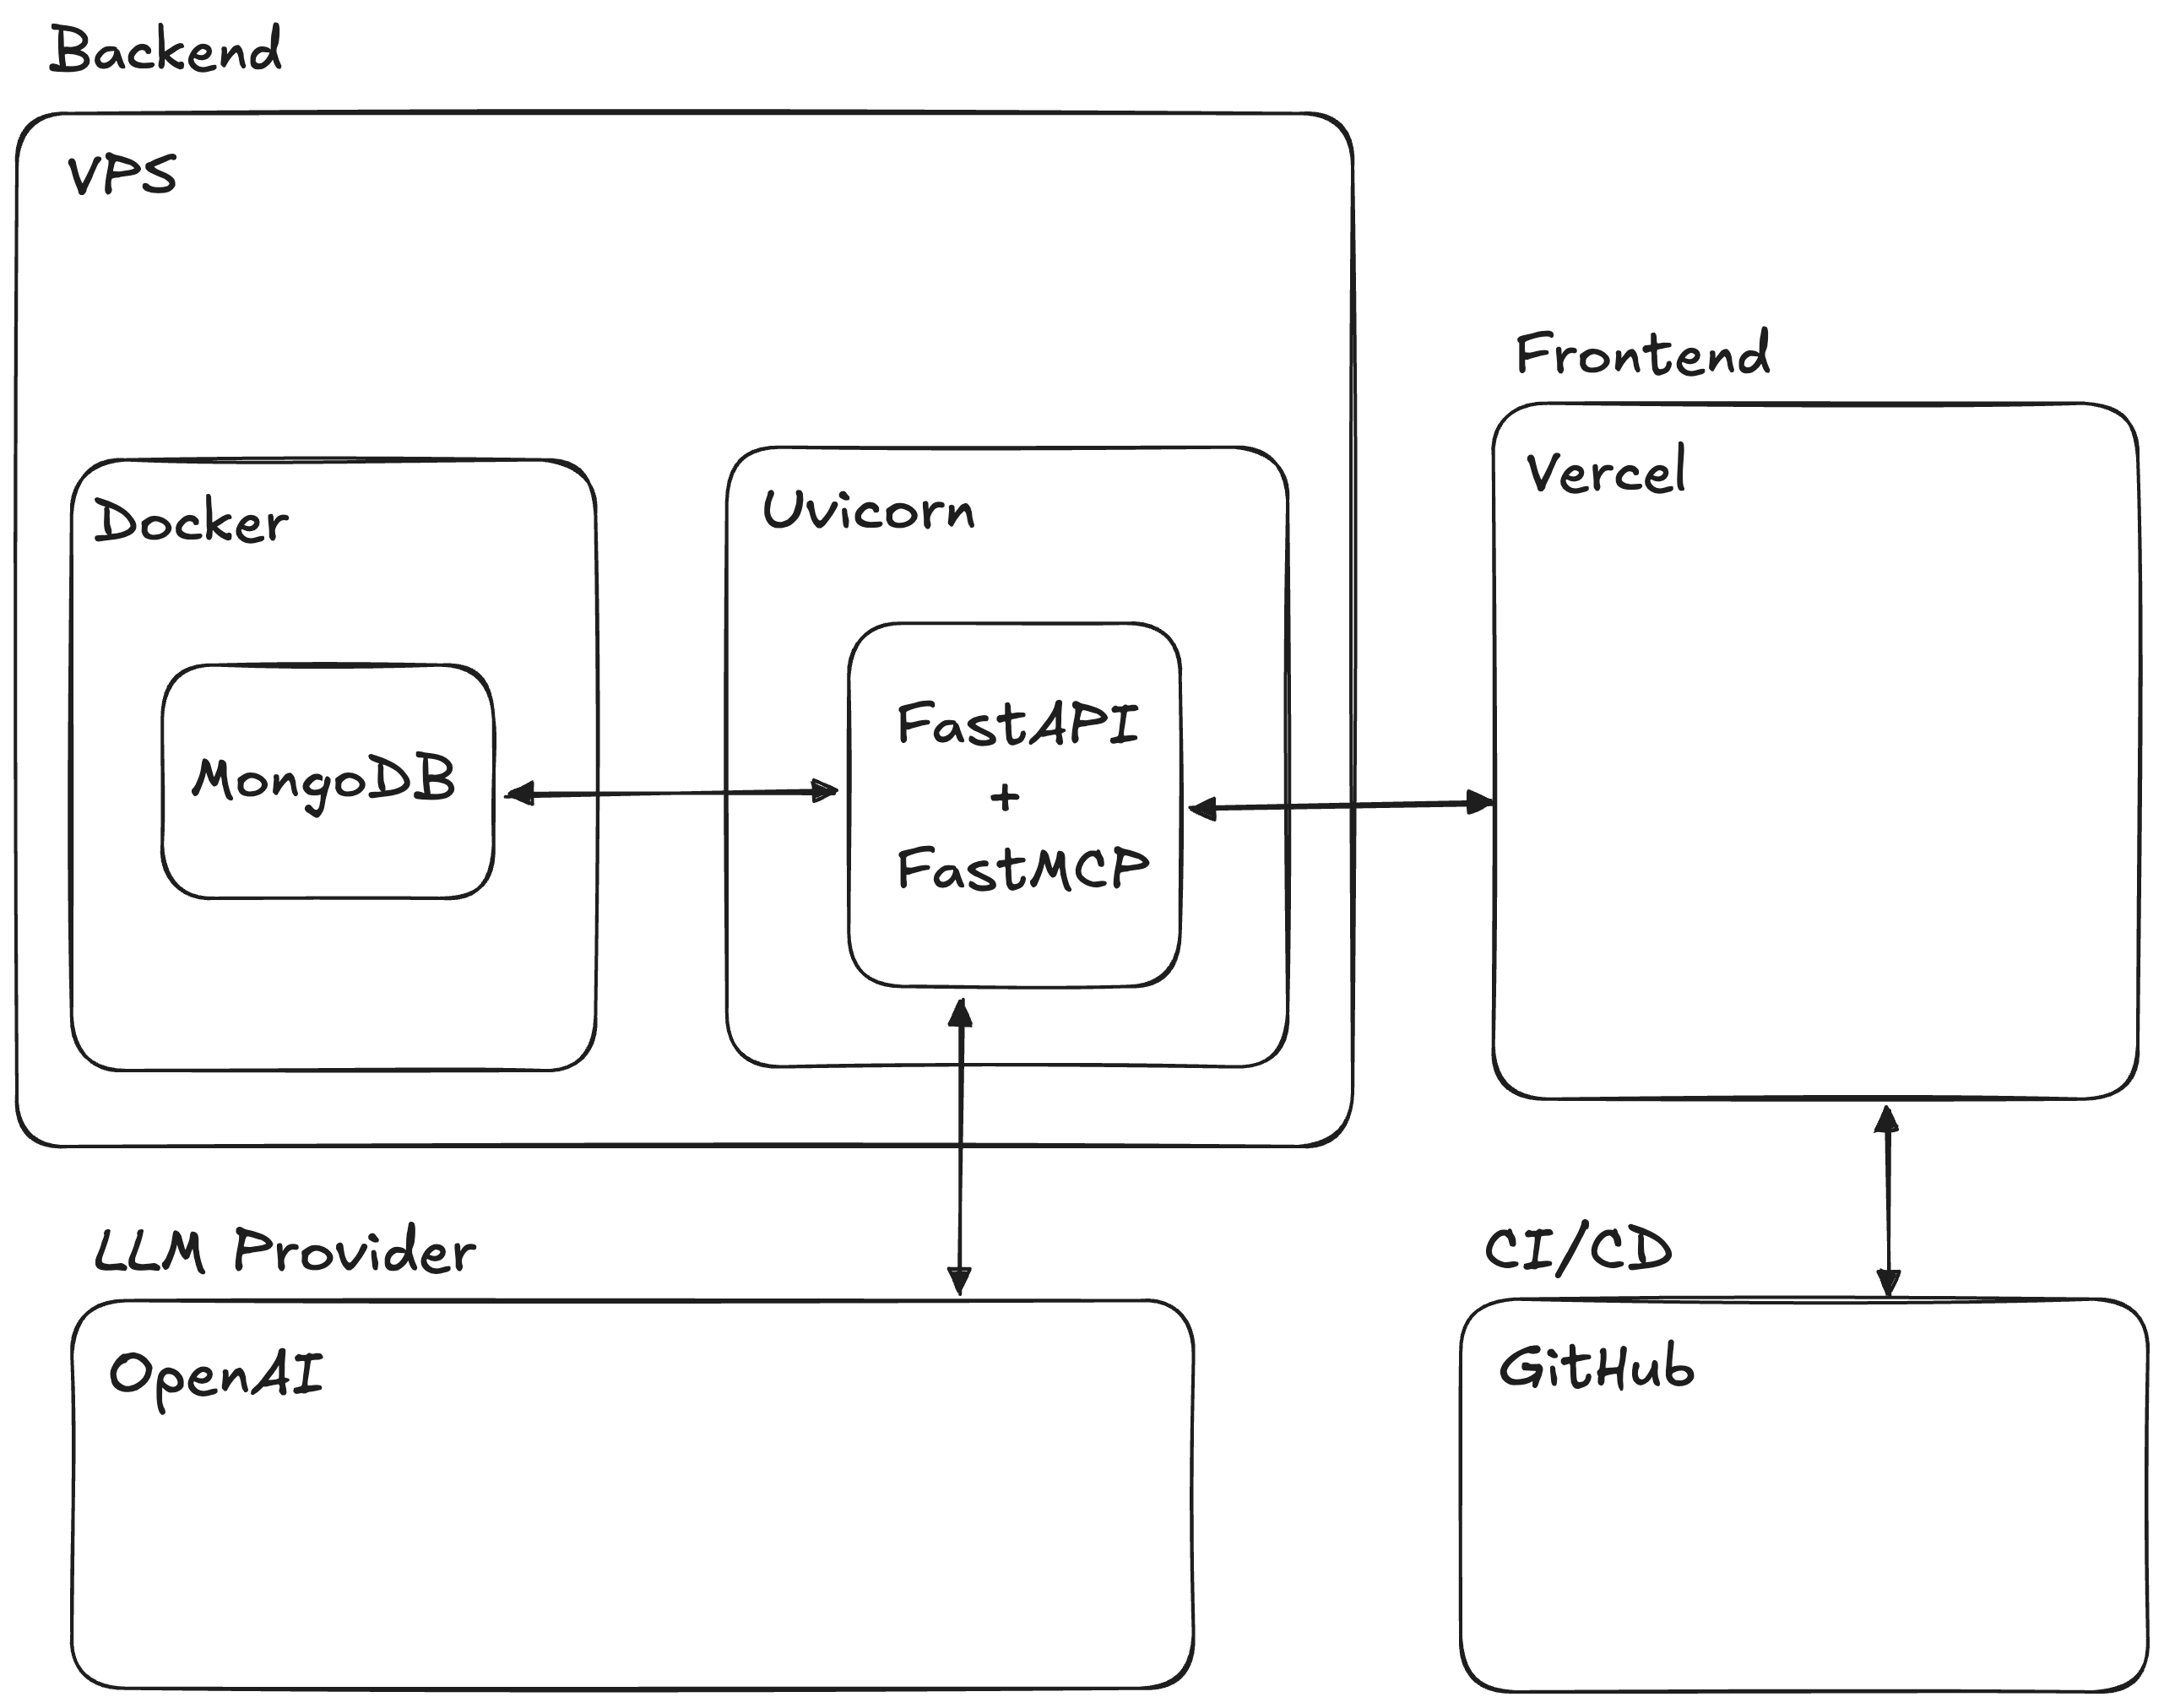
\includegraphics[width=0.9\textwidth]{imagenes/arch1.png}
  \caption{Arquitectura de la aplicación}
  \label{fig:arch1}
\end{figure}

\section{Backend}

El backend constituye el núcleo de la lógica de este trabajo. Se puede dividir en dos elementos: la base de datos MIMIC-IV almacenada en MongoDB con Docker, y la API RESTful con FastAPI que consulta datos, los procesa y los devuelve al cliente. También se encarga de llamar a los LLMs y a ejecutar el servidor MCP. Todo se aloja en un servidor personal y se accede por HTTPS gracias a Cloudflare Tunnels. A continuación profundizamos en esta parte del proyecto.

%\subsection{Almacenamiento de MIMIC-IV en MongoDB}
\subsection{MIMIC-IV en MongoDB}


Una de las tareas técnicas fundamentales del proyecto ha sido la migración del conjunto de datos, desde su formato original en archivos CSV comprimidos a una base de datos MongoDB. A continuación se explica todo el proceso.

\subsubsection{Entendiendo los datos}

MIMIC-IV recoge sus datos de distintas fuentes, y realiza todo un complejo proceso de conversión, transformación, anonimización, clasificación y corrección de los datos hasta obtener el resultado final \cite{MIMICIV_paper}.

\begin{figure}[H]
    \centering
    \fbox{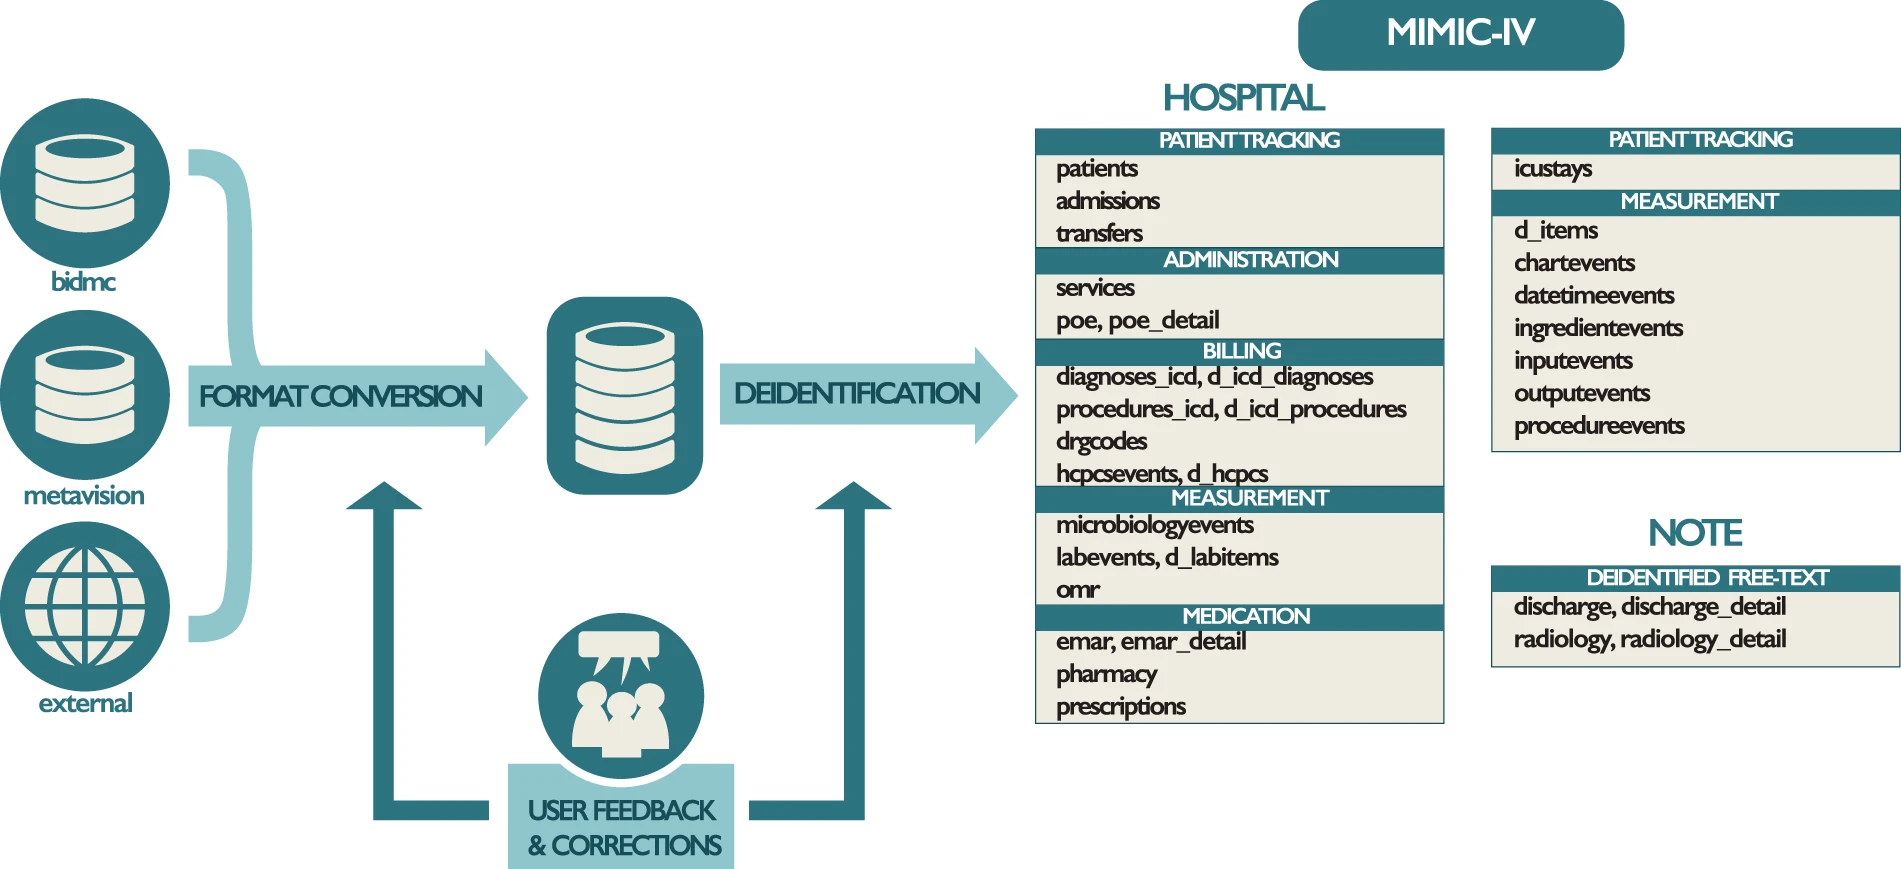
\includegraphics[width=0.95\textwidth]{imagenes/desarrolloMIMIC-IV.png}}
    %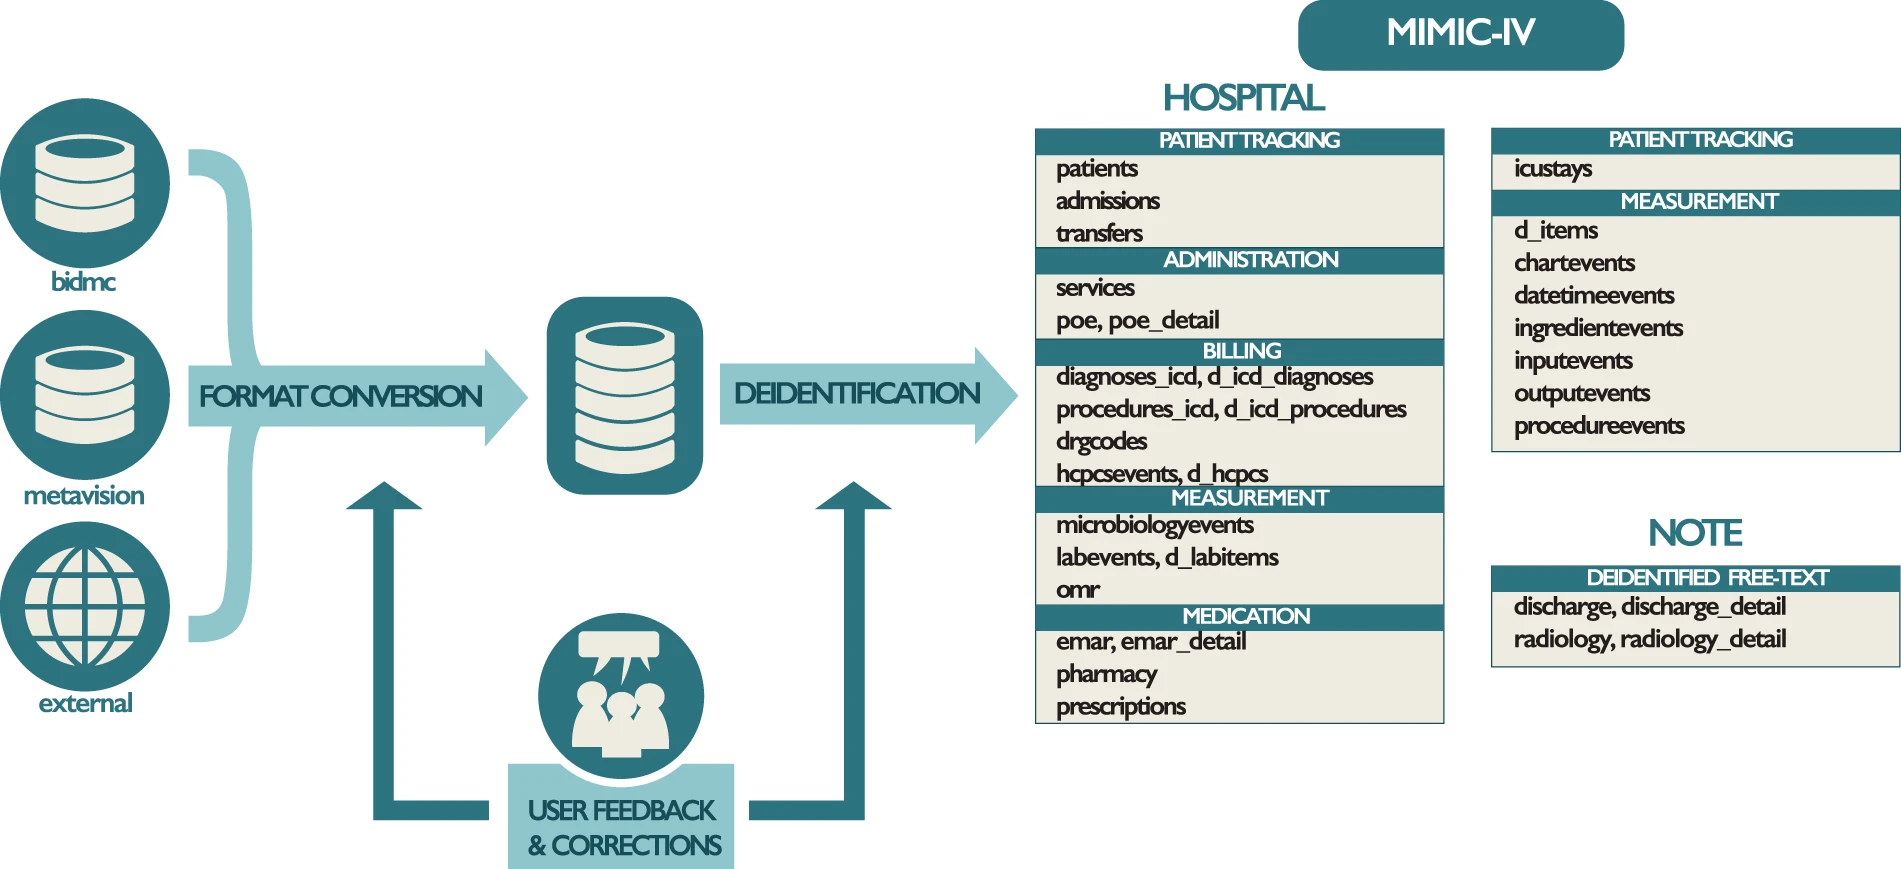
\includegraphics[width=0.95\textwidth]{imagenes/desarrolloMIMIC-IV.png}
    \caption{Resumen del proceso de desarrollo de MIMIC-IV.}
    \label{fig:desarrollo_mimiciv}
\end{figure}


Los datos, tal y como se han recibido, se estructuran módulos o ``carpetas", cada uno compuesto por diferentes tablas o ``archivos" que recogen distintos aspectos de la estancia hospitalaria del paciente. A continuación se resumen los dos módulos que se utilizan en el proyecto y sus tablas más relevantes:

\begin{itemize}
    \item \textbf{hosp}: Información hospitalaria general procedente del sistema de historia clínica electrónica. Incluye:
    \begin{itemize}
        \item \texttt{patients}: datos demográficos como sexo, edad y fecha de fallecimiento.
        \item \texttt{admissions}: detalles de los ingresos hospitalarios.
        \item \texttt{transfers}: movimientos de los pacientes entre distintas unidades.
        \item \texttt{labevents} y \texttt{d\_labitems}: resultados de laboratorio y su descripción.
        \item \texttt{microbiologyevents}: cultivos microbiológicos.
        \item \texttt{prescriptions}, \texttt{pharmacy}, \texttt{emar}, \texttt{emar\_detail}: información sobre prescripciones y administración de medicamentos.
        \item \texttt{diagnoses\_icd}, \texttt{d\_icd\_diagnoses}: diagnósticos realizados y codificados (ICD-9/10).
        \item \texttt{procedures\_icd}, \texttt{d\_icd\_procedures}: procedimientos realizados y codificados (ICD-9/10).
        \item \texttt{hcpcsevents}, \texttt{d\_hcpcs}, \texttt{drgcodes}: información de facturación y codificación hospitalaria.
        \item \texttt{services}: servicios hospitalarios responsables del paciente.
        \item \texttt{poe}, \texttt{poe\_detail}: órdenes médicas realizadas por los profesionales.
        \item \texttt{provider}, \texttt{omr}: información sobre proveedores y registros médicos online.
    \end{itemize}
    \item \textbf{icu}: Datos recogidos específicamente durante la estancia en la UCI, provenientes del sistema clínico MetaVision. Incluye:
    \begin{itemize}
        \item \texttt{icustays}: información sobre las estancias en UCI.
        \item \texttt{chartevents}: registros detallados de constantes, procedimientos, observaciones y eventos clínicos.
        \item \texttt{inputevents}, \texttt{ingredientevents}: administración de fluidos, nutrición y medicamentos intravenosos.
        \item \texttt{outputevents}: registros de salidas del paciente (orina, drenajes, etc.).
        \item \texttt{procedureevents}: procedimientos realizados en UCI.
        \item \texttt{datetimeevents}: eventos documentados con fecha y hora.
        \item \texttt{d\_items}: diccionario de variables y conceptos registrados en los eventos.
        \item \texttt{caregiver}: identificadores de los profesionales sanitarios en UCI.
    \end{itemize}
\end{itemize}



En nuestro caso, utilizamos estos dos módulos pero hay más, como \textbf{ed} (emergency department), \textbf{cxr} (radiografías de tórax) y \textbf{note} (notas clínicas desidentificadas), que amplían la información disponible para cada paciente.

Un aspecto fundamental para trabajar con MIMIC-IV es la correcta utilización de los campos identificadores que permiten relacionar la información entre tablas y reconstruir la trayectoria clínica de cada paciente:

\begin{itemize}
    \item \texttt{subject\_id}: identificador único de paciente, presente en prácticamente todas las tablas. Permite agrupar toda la información relativa a una misma persona a lo largo de distintas estancias y episodios.
    \item \texttt{hadm\_id}: identificador único de cada ingreso hospitalario. Cada hospitalización de un paciente tiene uno distinto, lo que permite diferenciar varios ingresos de la misma persona y asociar eventos, pruebas y tratamientos concretos a cada episodio.
    \item \texttt{stay\_id} (en ICU): identifica de forma única cada estancia en la UCI, permitiendo enlazar los eventos críticos de cuidados intensivos.
    \item Otros identificadores secundarios: \texttt{specimen\_id} (muestras de laboratorio), \texttt{pharmacy\_id}, \texttt{order\_provider\_id} (profesional que ordena una prueba o medicación), \texttt{itemid} (tipo de medición o concepto registrado), entre otros.
\end{itemize}

Además de todos estos datos, los tutores del trabajo proporcionaron otro archivo \texttt{icd\_equivalencias}, el cual contiene las equivalencias entre códigos ICD-9 e ICD-10. Los códigos ICD (International Classification of Diseases) son el estándar internacional para clasificar enfermedades, diagnósticos y procedimientos médicos. Esta tabla permite unificar datos codificados en ambas versiones y aporta una clasificación jerárquica organizada en capítulos (chapters), supersecciones (super sections) y secciones (sections). Por ejemplo, el código ICD-9 ``0090'' (Infectious colitis, enteritis, and gastroenteritis) se mapea al ICD-10 ``A09'' y se clasifica dentro del capítulo ``A'' (Certain infectious and parasitic diseases), supersección ``A00-A09'' (Intestinal infectious diseases) y sección ``A09'' (Infectious gastroenteritis and colitis, unspecified). Esta estructura facilita el análisis y visualización de diagnósticos por categorías médicas.

En conclusión, toda esta estructura modular nos permite, a nivel de paciente, reconstruir de forma detallada la trayectoria clínica, desde su ingreso hasta el alta, pasando por episodios críticos, pruebas, tratamientos y evolución. A nivel global, las posibilidades son enormes, para calcular estadísticas, visualizaciones, y todo tipo de agregaciones de las que se pueda extraer conocimiento. Para más detalles sobre los datos, puede consultarse la documentación oficial de MIMIC-IV \cite{MIMICIV_docs}.

\subsubsection{Desplegando MongoDB}

Para el despliegue de MongoDB se utilizan dos contenedores Docker, en distintos puertos, uno para la versión completa del conjunto de datos, y otro para la versión demo, facilitando así la realización de pruebas sin tener que lidiar con los cientos de millones de datos de la versión completa. Como apoyo al desarrollo, y también en forma de contenedores, se despliegan las herramientas de interfaz gráfica: Portainer para Docker \cite{portainer_ce} y Mongo Express para las bases de datos \cite{mongo_express}. 


\begin{figure}[H]
  \centering
  \fbox{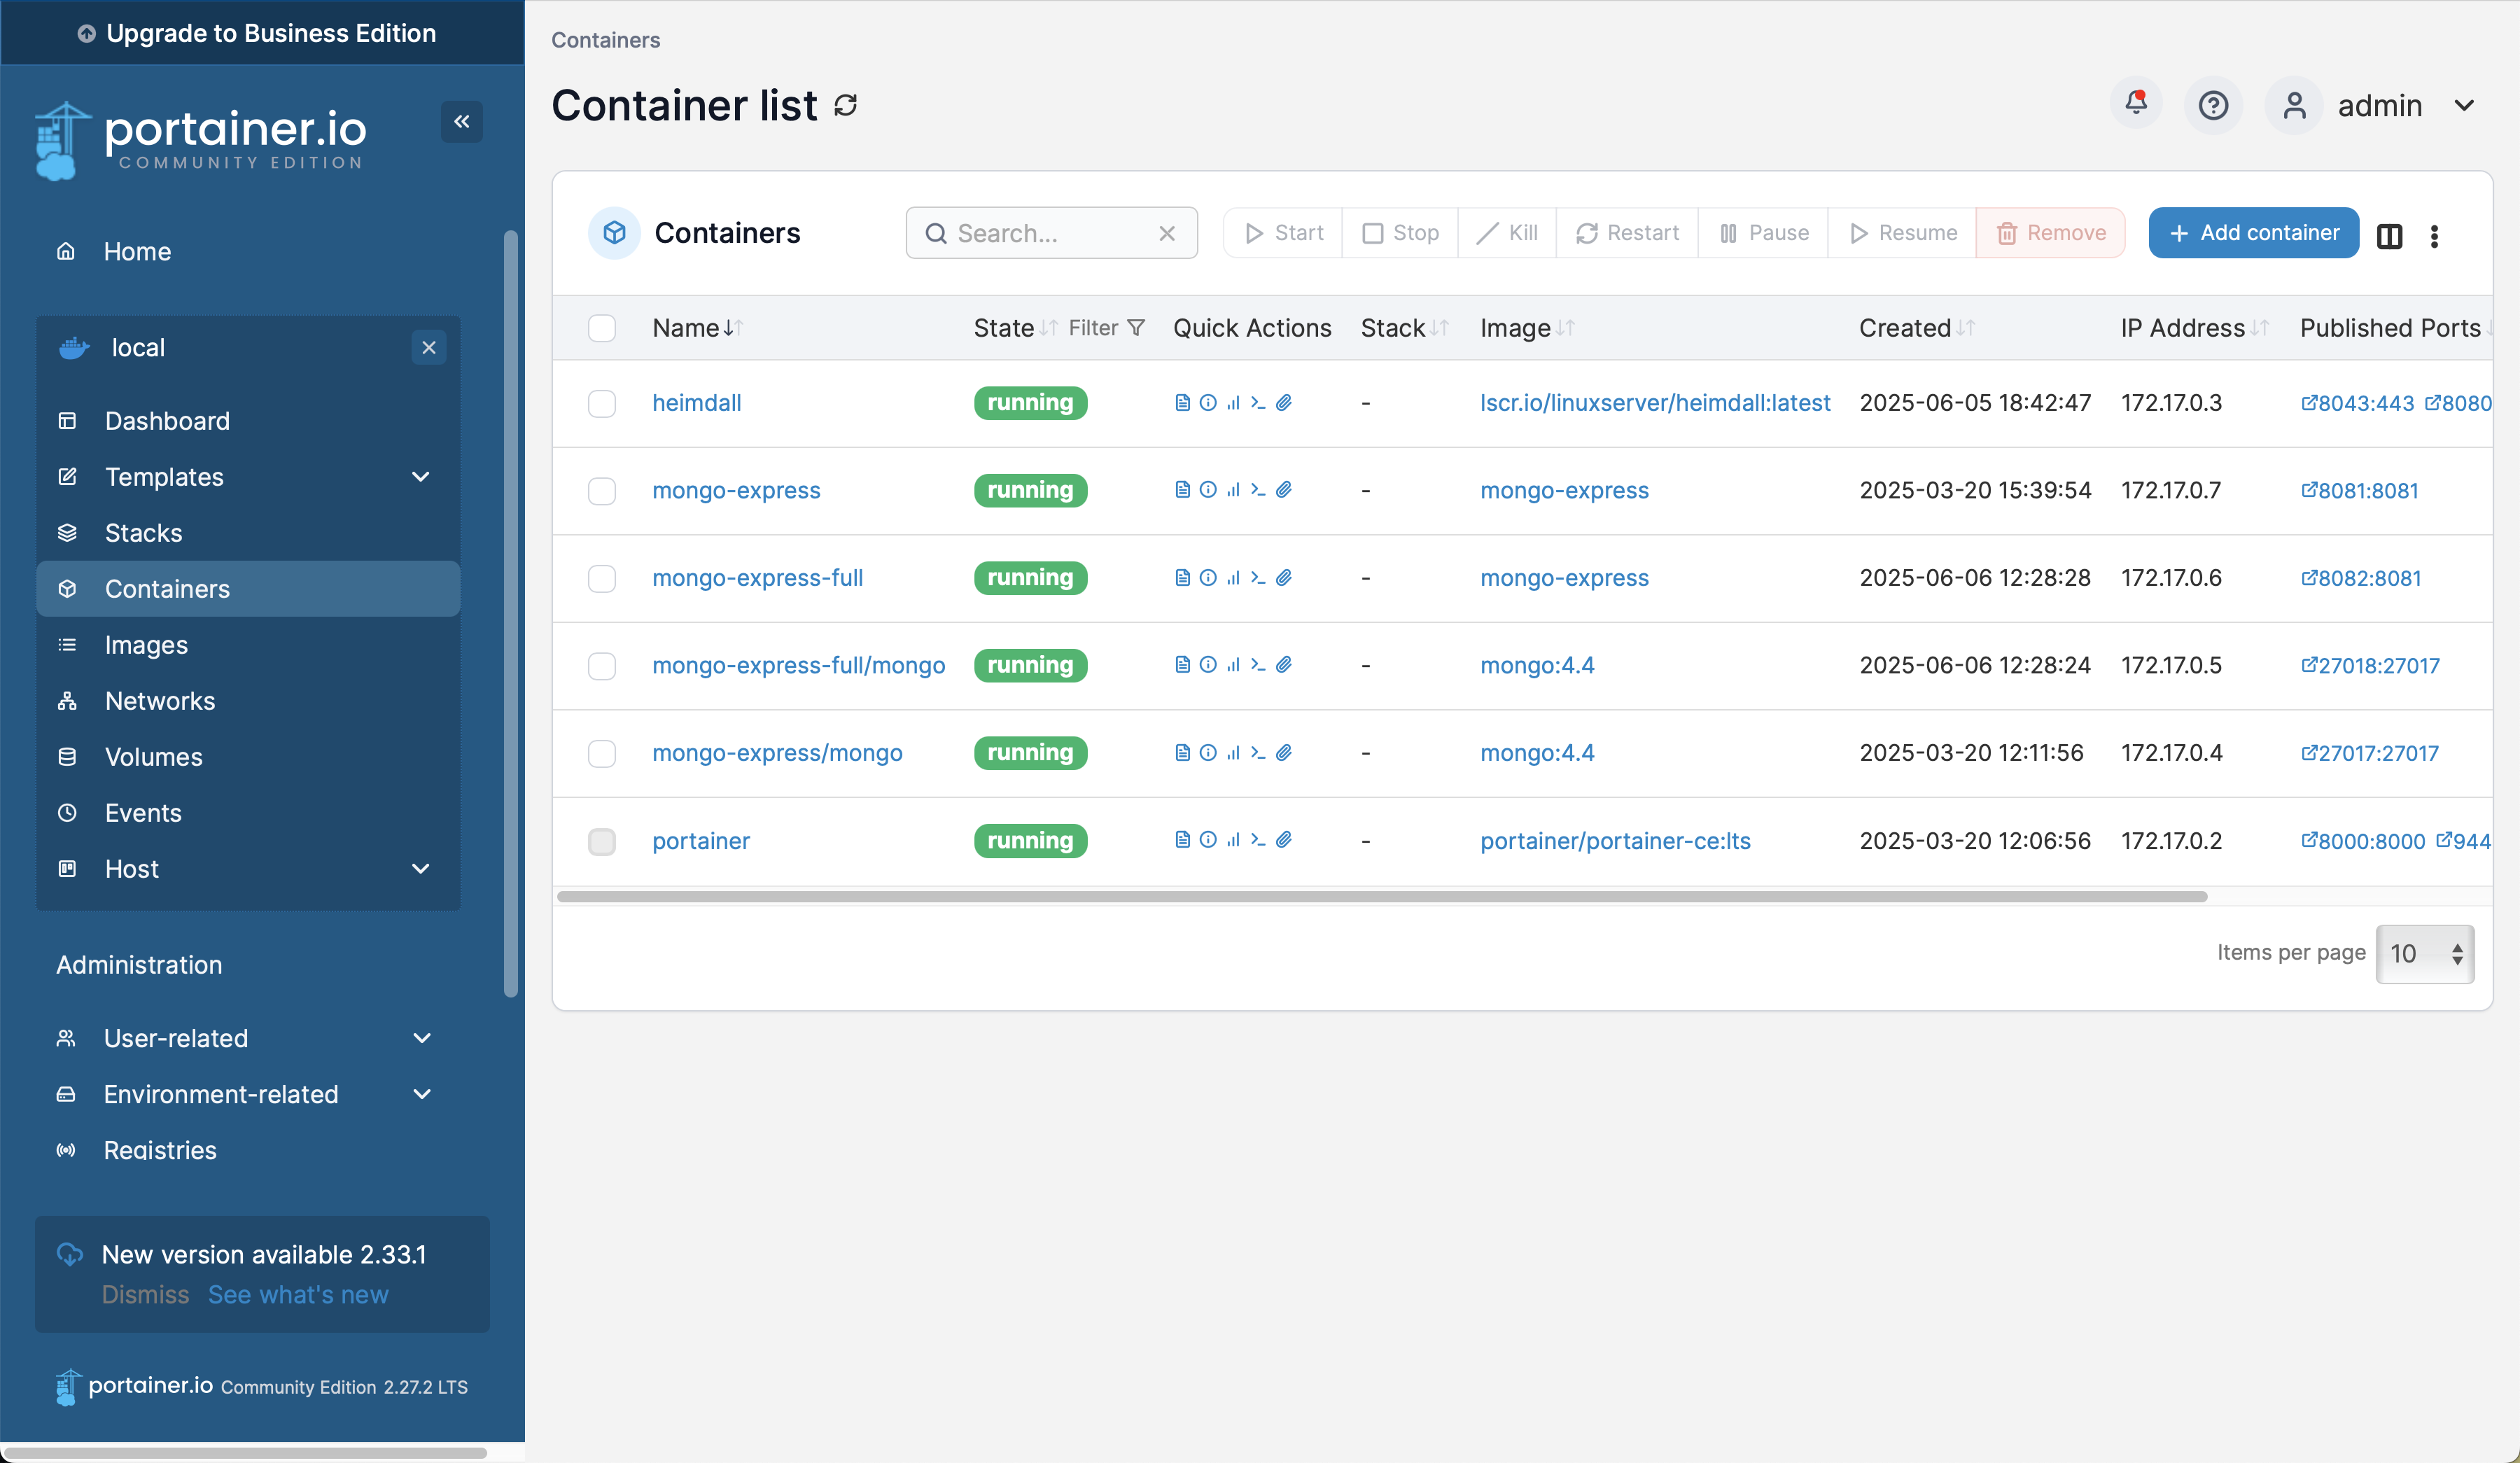
\includegraphics[width=1\textwidth]{imagenes/screenshot3.png}}
  %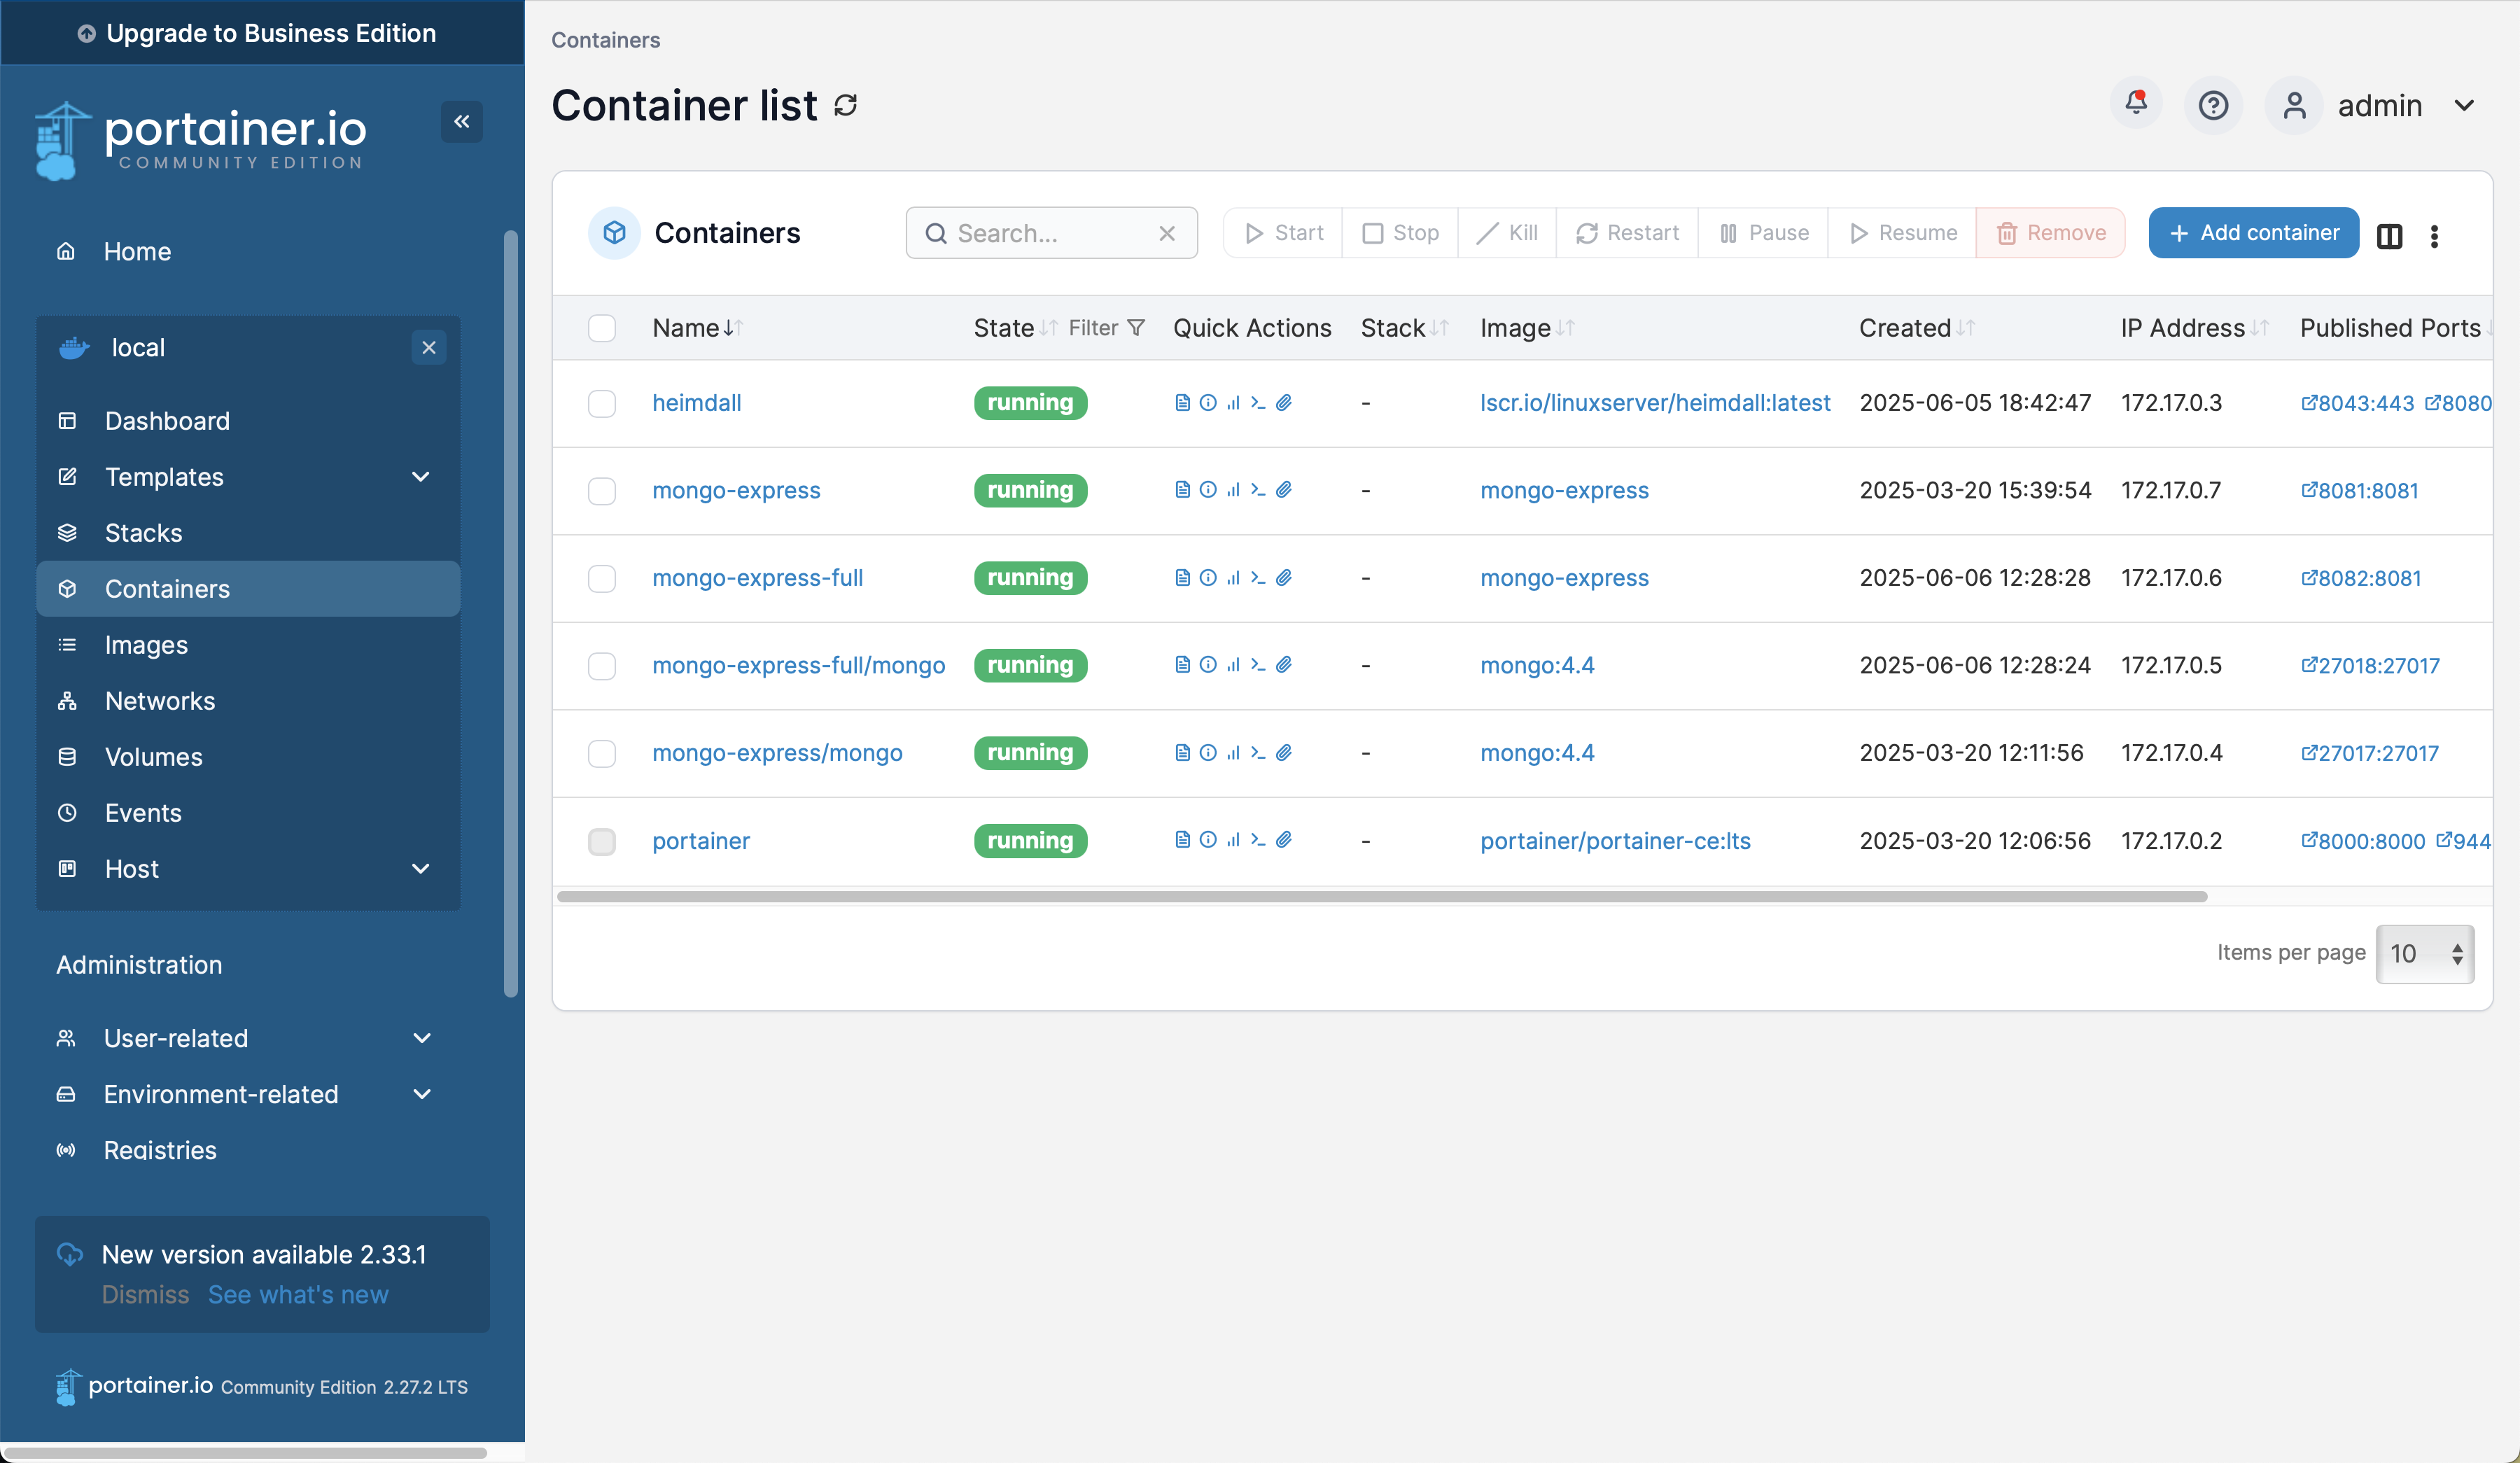
\includegraphics[width=1\textwidth]{imagenes/screenshot3.png}
  \caption{Captura de pantalla de Portainer}
  \label{fig:screenshot3}
\end{figure}


% --------------------
\subsubsection{El proceso de migración}

Se realizó mediante scripts de Python utilizando la librería \texttt{pandas} para la lectura de archivos CSV y \texttt{pymongo} para la inserción en MongoDB. Cada fila del CSV se convierte en un archivo JSON/BSON \cite{mongojsonbson} en MongoDB, donde cada columna es un campo del documento, y cada archivo CSV completo acaba siendo una colección de documentos. Podemos entenderlo mejor, pensando que cada archivo CSV es equivalente a una tabla de una base de datos relacional, y observando la siguiente figura \ref{fig:equivalenciasql}.

\begin{figure}[H]
  \centering
  \fbox{\includegraphics[width=0.8\textwidth]{imagenes/mongodb-vs-sql-1.png}}
  %\includegraphics[width=0.8\textwidth]{imagenes/mongodb-vs-sql-1.png}
  \caption{Equivalencia entre conceptos SQL y NoSQL \cite{equisqlfoto}}
  \label{fig:equivalenciasql}
\end{figure}

Los nombres de las colecciones recibieron el formato \texttt{\textless módulo\textgreater\_\textless tabla\textgreater}. Por ejemplo: \texttt{hosp\_patients}, \texttt{icu\_procedureevents}, etc.

\begin{figure}[H]
  \centering
  \fbox{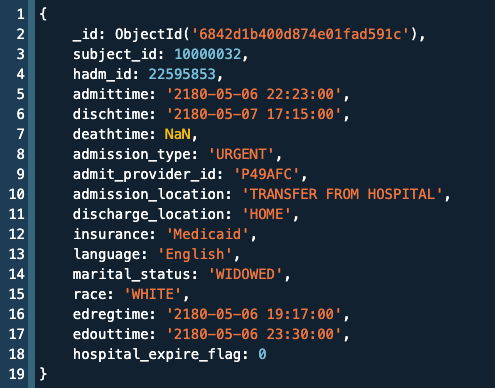
\includegraphics[width=0.6\textwidth]{imagenes/ej_admission.png}}
  %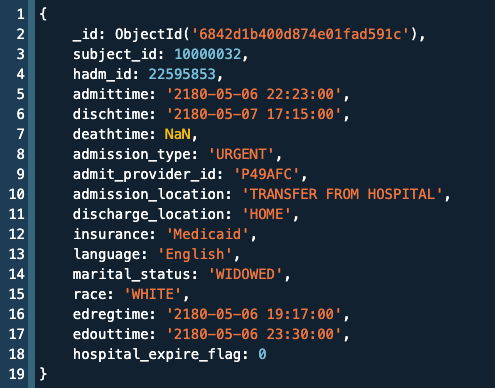
\includegraphics[width=0.6\textwidth]{imagenes/ej_admission.png}
  \caption{Ejemplo de un documento de \texttt{hosp\_admissions}}
  \label{fig:screenshot3}
\end{figure}

Una vez entendida la estructura de los datos de MIMIC-IV, la equivalencia de los archivos CSV a documentos y colecciones de MongoDB, la base de datos ejecutandose con Docker y los scripts preparados, era momento de realizar la migración. 

Todo este proceso se realizó dos veces, para dos versiones distintas de MIMIC-IV: la versión completa, cuyo acceso está restringido y contiene múltiples GBs de información, y la versión demo, que es un subset de 100 pacientes y es de acceso libre \cite{MIMICIV_Demo}. Para la versión completa, el procesamiento se tuvo que realizar por chuncks para evitar el desbordamiento de memoria, que fue un problema recurrente debido a la cantidad masiva de datos.

\begin{figure}[H]
    \centering
    \fbox{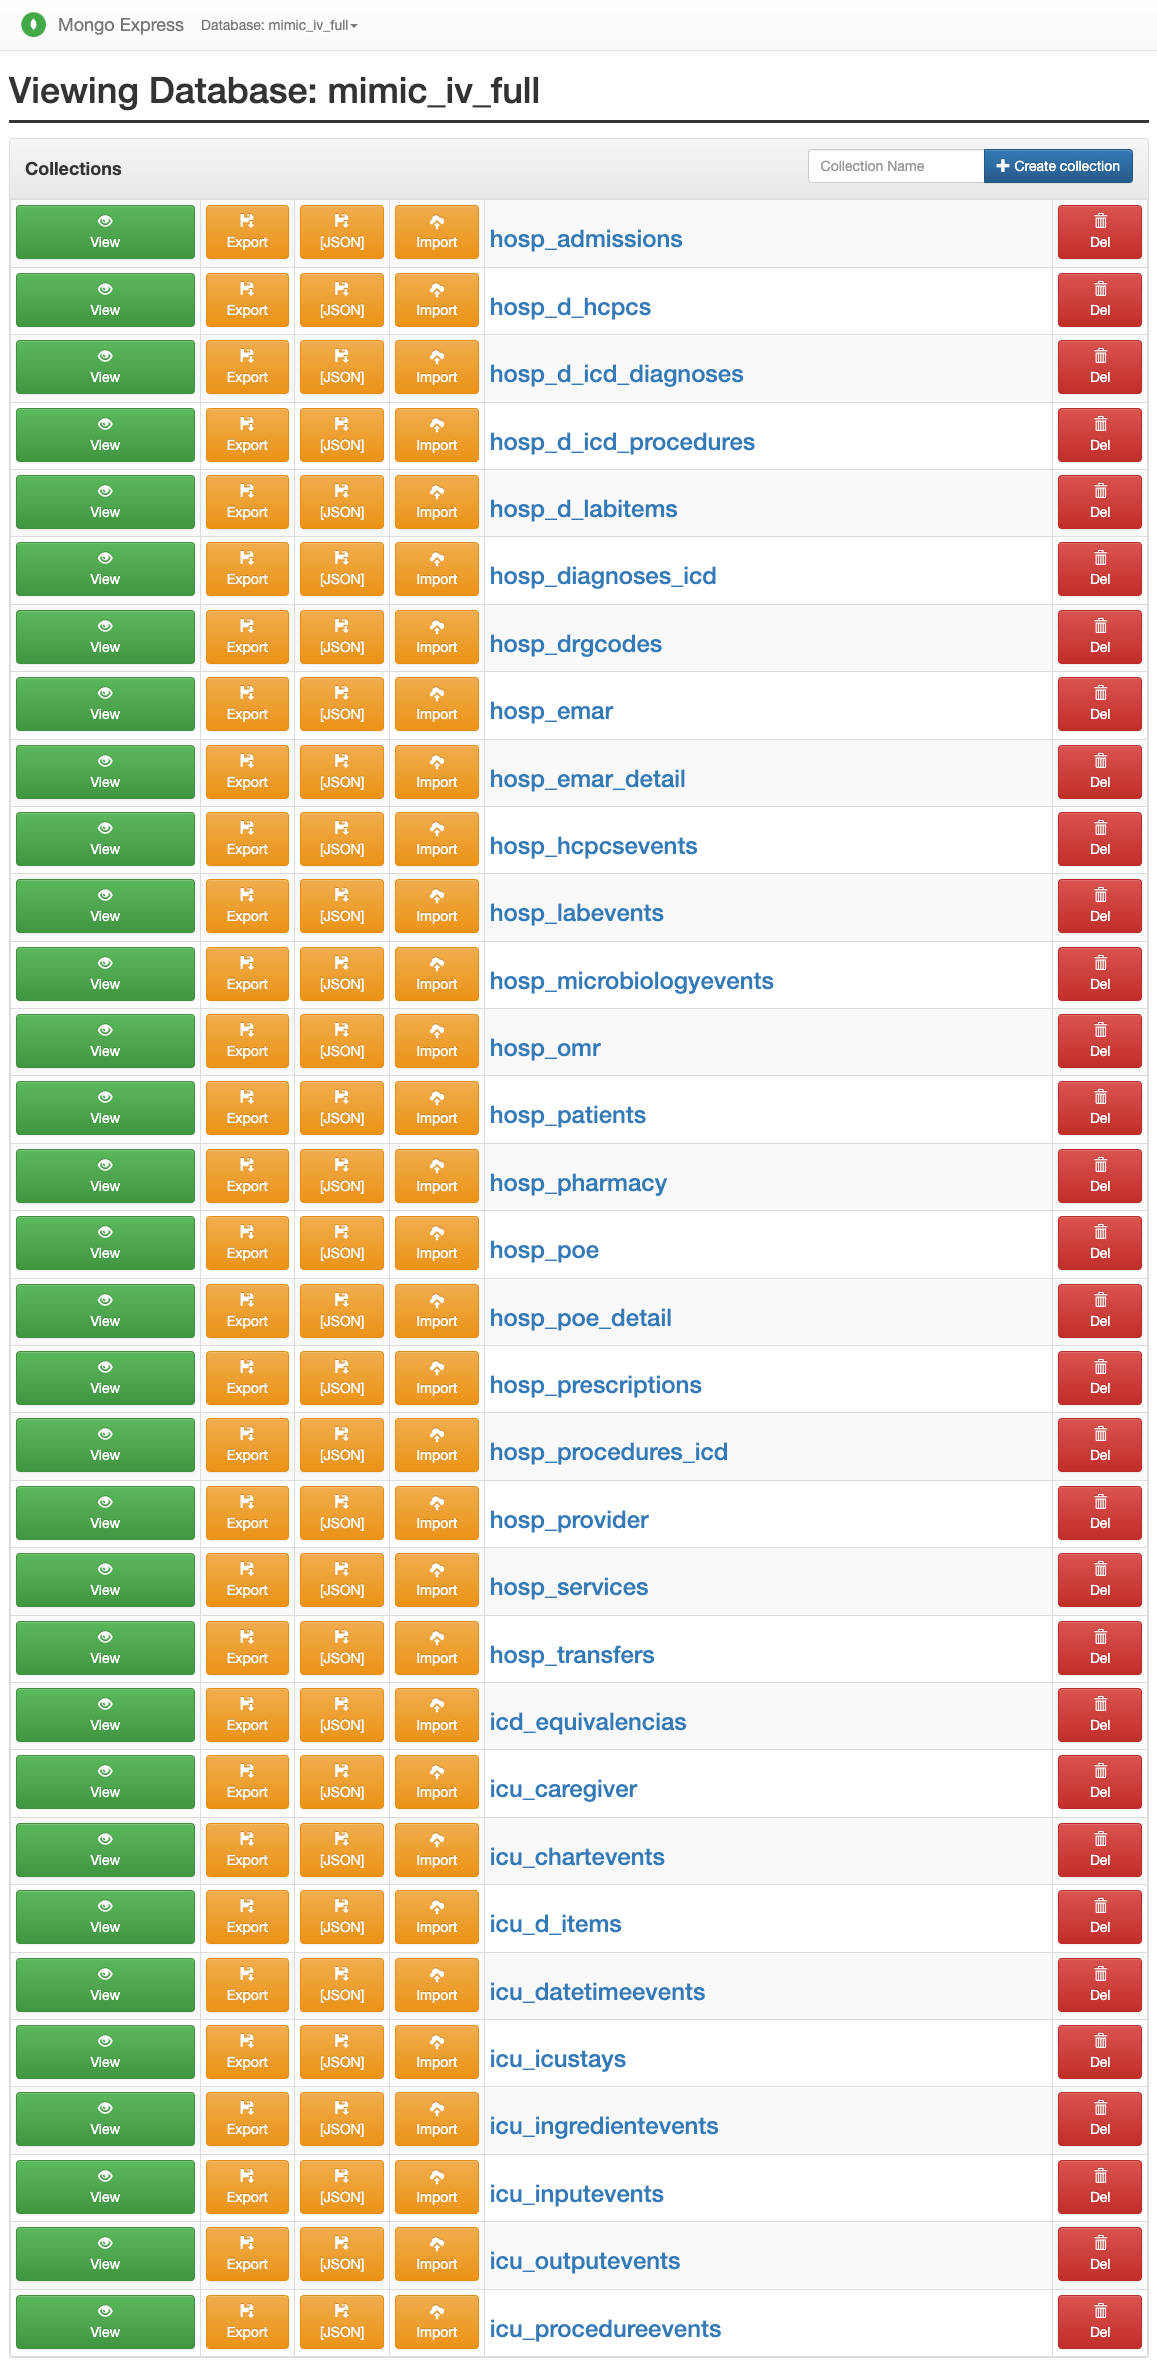
\includegraphics[width=0.8\textwidth]{imagenes/db_full_list.png}}
    %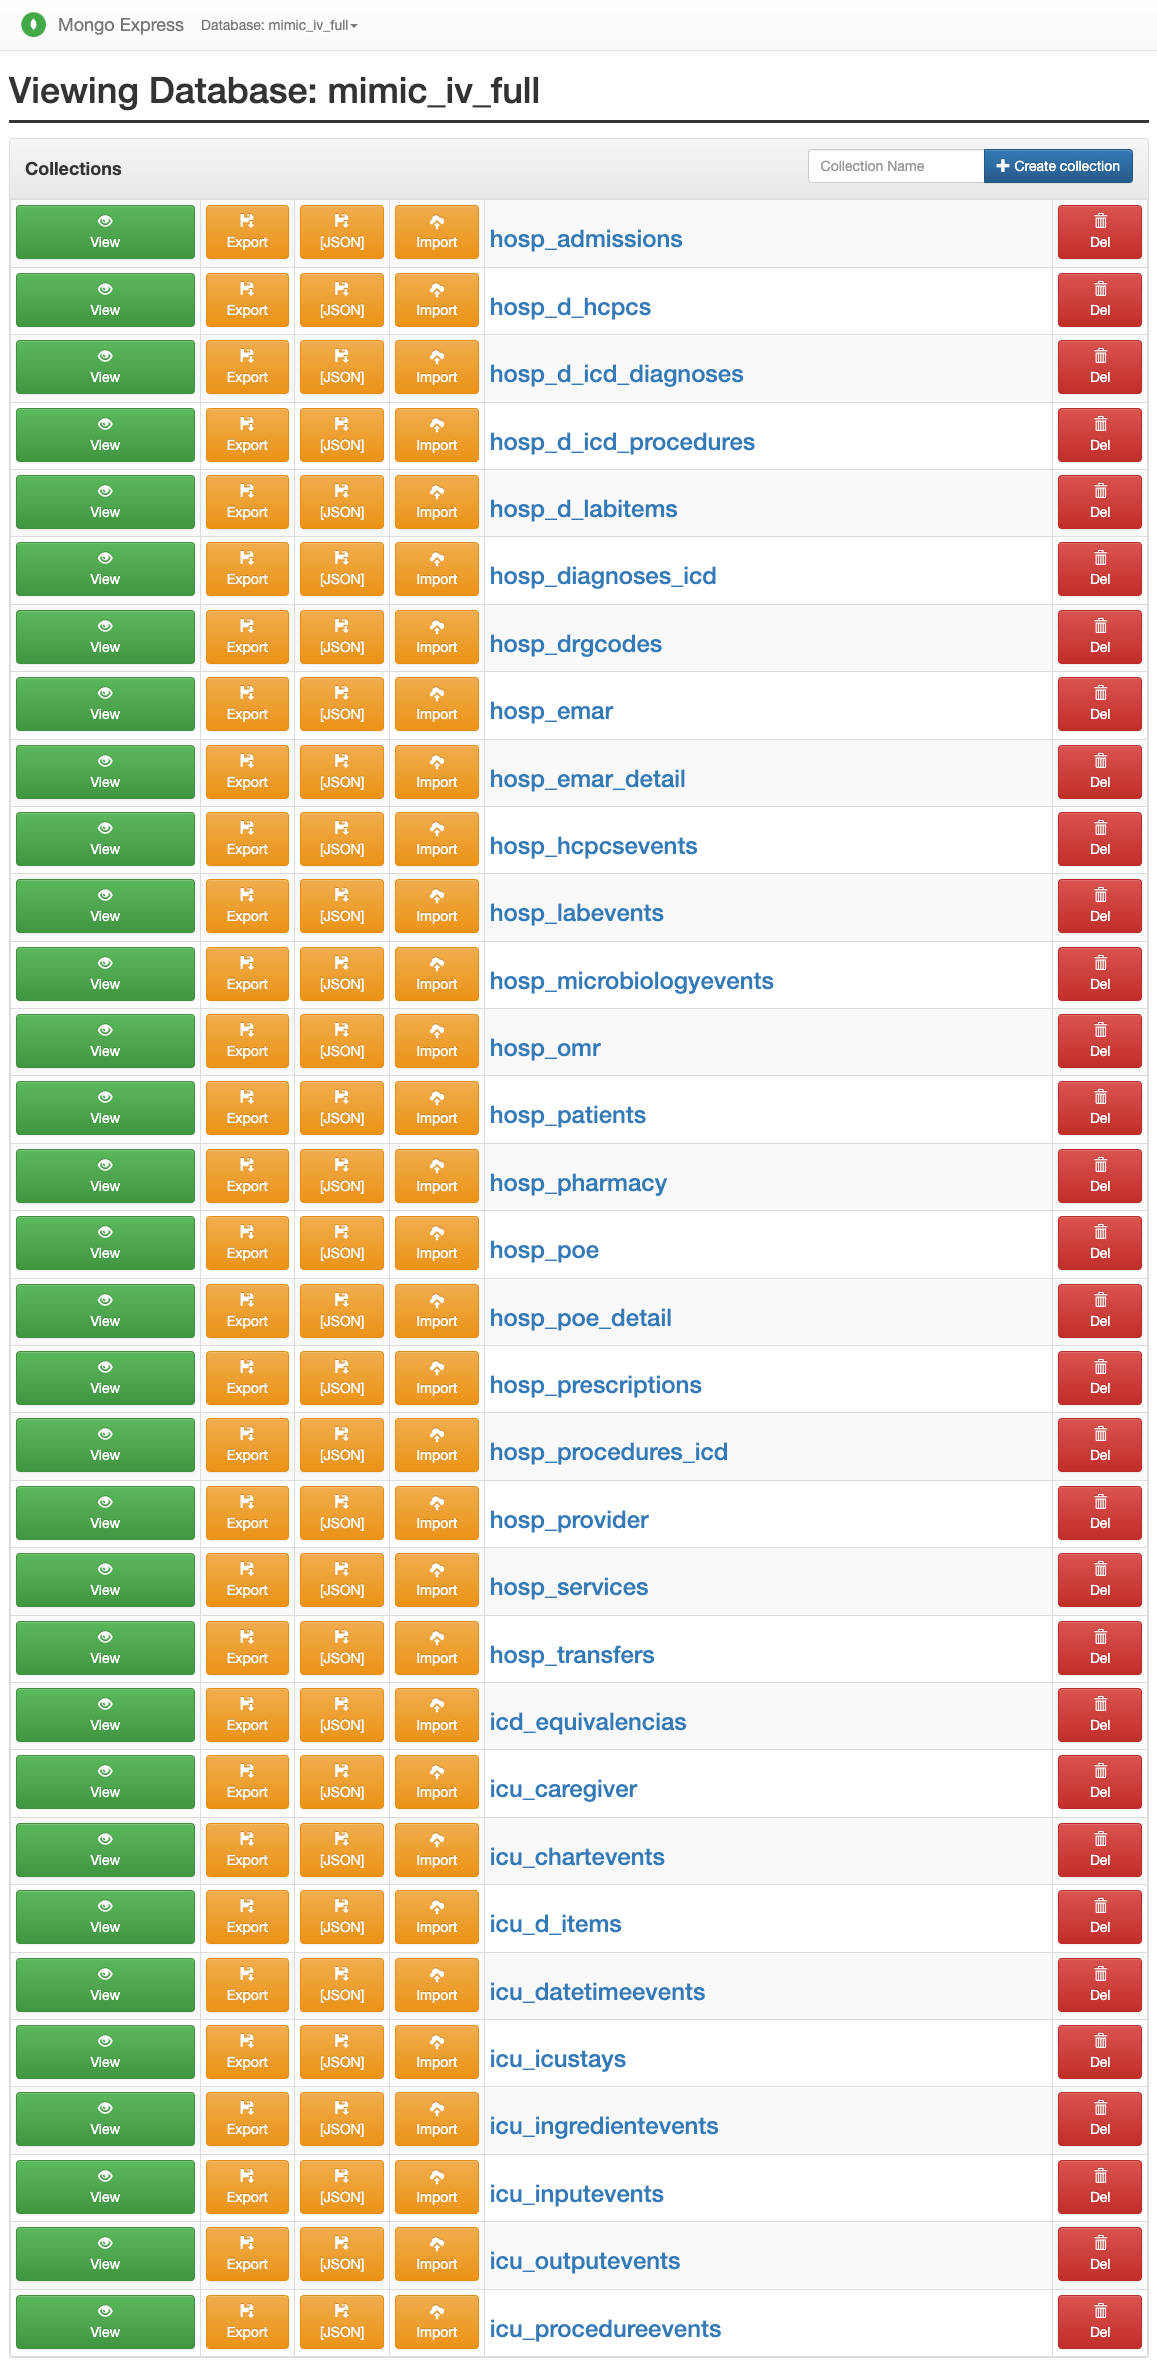
\includegraphics[width=0.8\textwidth]{imagenes/db_full_list.png}
    \caption{Colecciones resultantes tras la importacion. Captura de pantalla de la interfaz de Mongo Express.}
    \label{fig:db_full_list}
\end{figure}

\begin{figure}[H]
    \centering
    \fbox{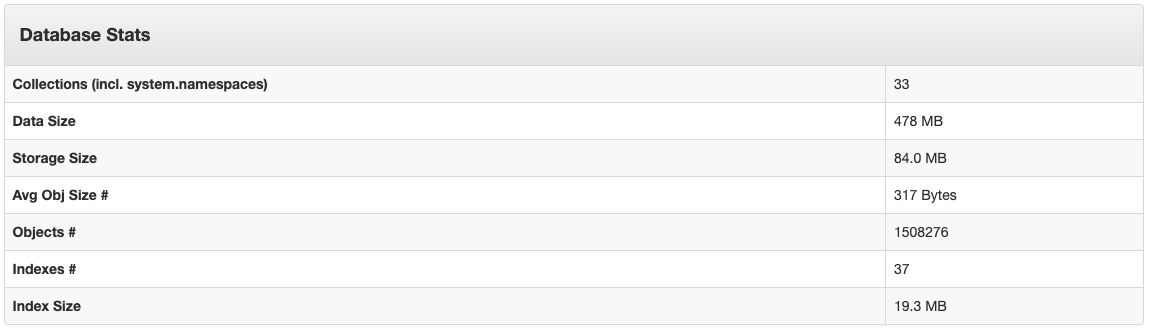
\includegraphics[width=1\textwidth]{imagenes/stats_demo.png}}
    %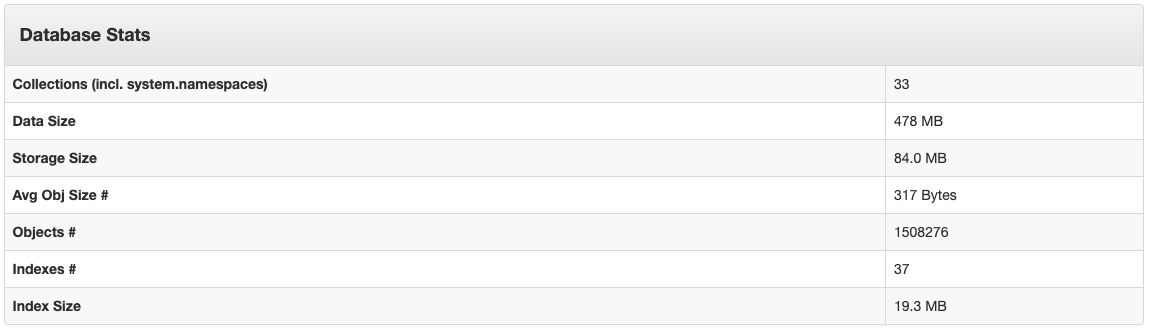
\includegraphics[width=1\textwidth]{imagenes/stats_demo.png}
    \caption{Estadísticas de la versión demo de la base de datos.}
    \label{fig:stats_demo}
\end{figure}

\begin{figure}[H]
    \centering
    \fbox{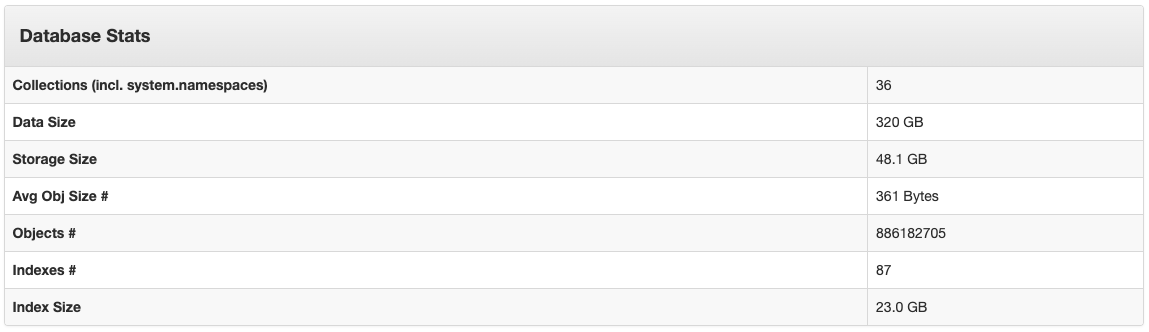
\includegraphics[width=1\textwidth]{imagenes/stats_full.png}}
    %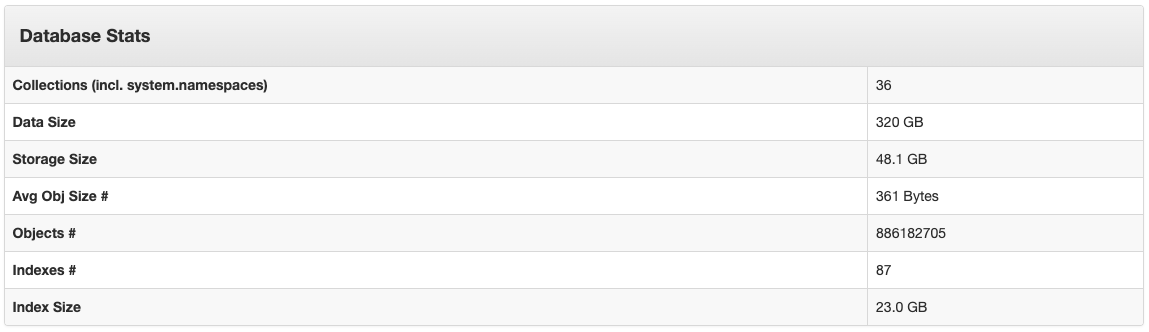
\includegraphics[width=1\textwidth]{imagenes/stats_full.png}
    \caption{Estadísticas de la versión completa de la base de datos.}
    \label{fig:stats_full}
\end{figure}


Además de las colecciones base que obtenemos de MIMIC-IV, a lo largo del proyecto se agregaron manualmente algunas más, necesarias tanto para pruebas como para algunas visualizaciones, de las que se hablará más tarde. Por eso, las estadísticas mostradas en las dos figuras anteriores, no coinciden exactamente con las del estado inicial del proyecto. 

También se crearon manualmente múltiples índices para optimizar el rendimiento de las consultas. Los índices en MongoDB funcionan de manera similar a los índices de un libro: crean estructuras de datos ordenadas que permiten localizar documentos específicos sin tener que examinar toda la colección. Esto es especialmente crítico en MIMIC-IV debido al volumen masivo de datos, donde algunas colecciones como \texttt{icu\_chartevents} contienen decenas de millones de registros. Por ejemplo, se crearon índices sobre campos clave como \texttt{subject\_id} (para consultas por paciente), \texttt{hadm\_id} (para ingresos hospitalarios), \texttt{charttime} (para búsquedas temporales) y \texttt{itemid} (para tipos específicos de mediciones). Sin estos índices, una consulta que busque todos los signos vitales de un paciente específico tendría que examinar millones de documentos, mientras que con el índice correspondiente la búsqueda se realiza en milisegundos.


En resumen, con esta implementación, se ha logrado transformar exitosamente el conjunto de datos MIMIC-IV desde su formato original en archivos CSV a una base de datos MongoDB completamente funcional y optimizada. La combinación de una estructura de datos bien comprendida, índices estratégicamente ubicados y colecciones auxiliares especializadas proporciona una base sólida para el procesamiento eficiente de consultas complejas sobre grandes volúmenes de datos clínicos. Esta infraestructura de datos establece los cimientos para el siguiente componente del sistema: la API RESTful que permitirá acceder, procesar y servir esta información de manera estructurada y escalable.





%Por ejemplo, el número total de colecciones esperado al comienzo es de 32 (22 del módulo \texttt{hosp}, 9 del módulo \texttt{icu} y 1 de \texttt{icd\_equivalencias}. 
%@todo: en que punto voy a hablar de las colecciones nuevas que he añadido yo -> aqui mismo -> NO, cuando hable de cada visualizacion



%\begin{figure}[H]
%  \centering
%  \fbox{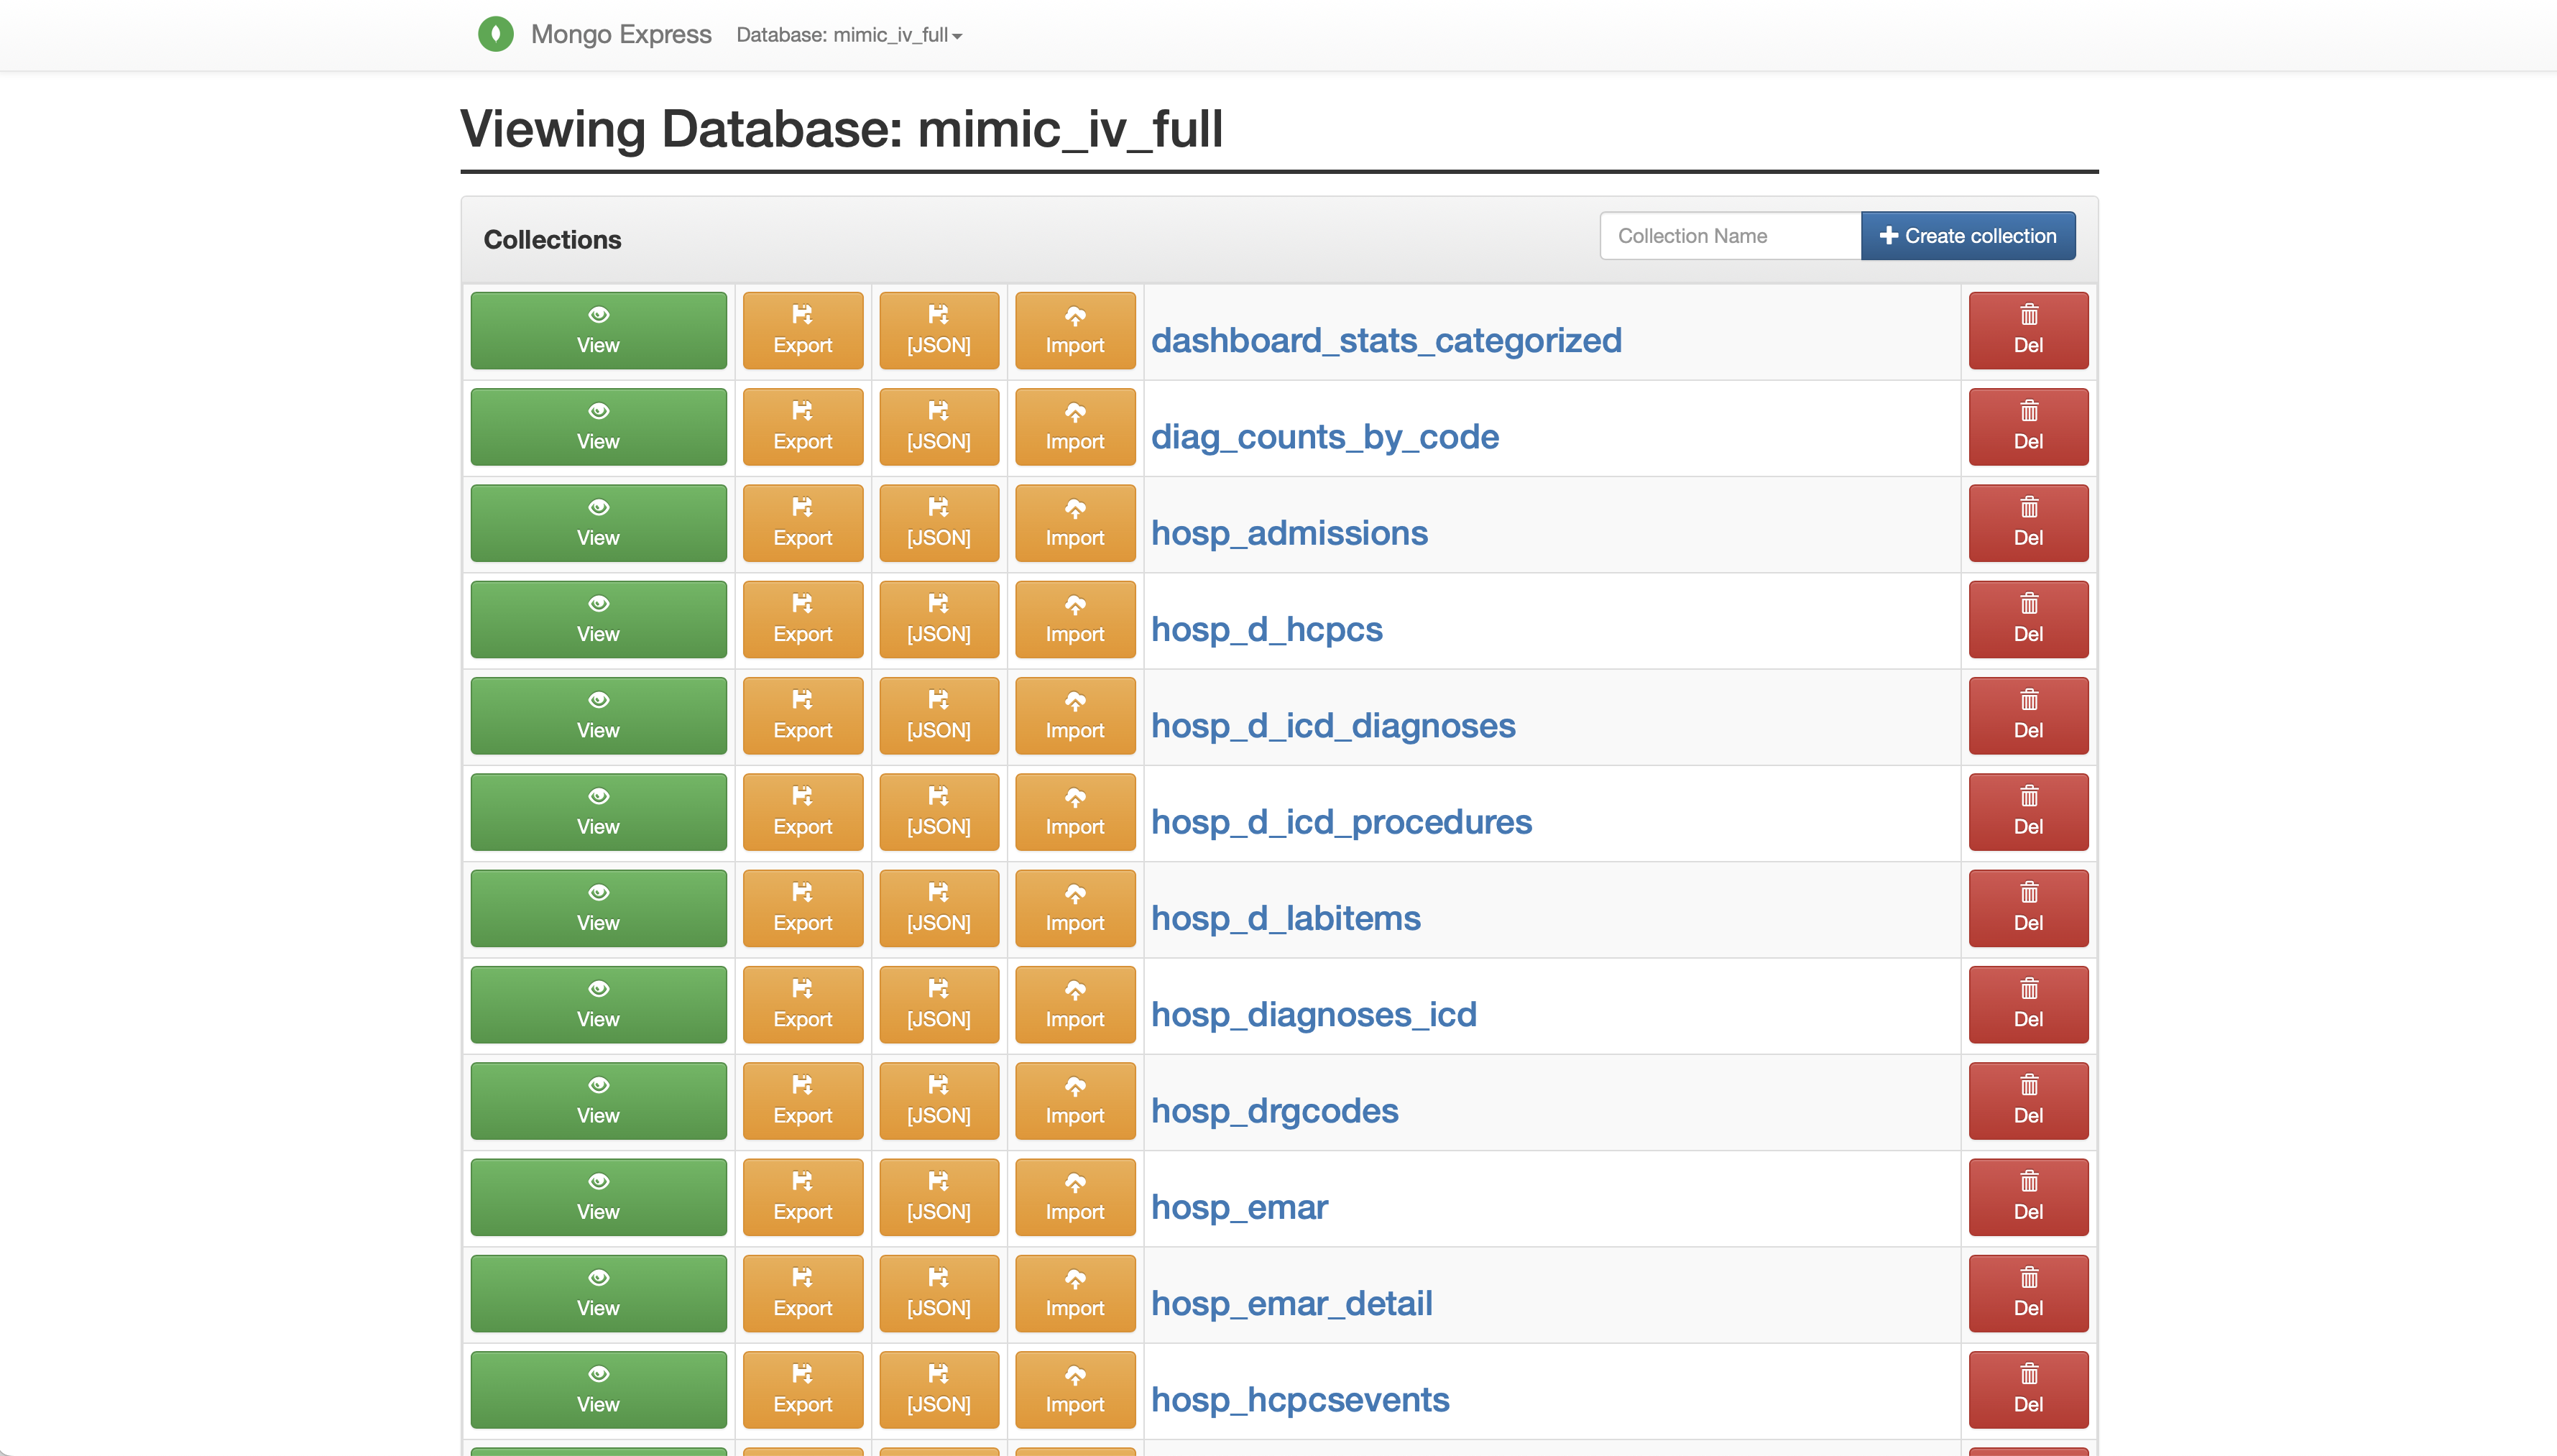
\includegraphics[width=1\textwidth]{imagenes/screenshot2.png}}
%  \caption{Captura de pantalla de Mongo Express}
%  \label{fig:screenshot2}
%\end{figure}


\subsection{API RESTful}

La API que obtiene, procesa y sirve los datos está construida sobre FastAPI \cite{fastapi}, un framework moderno que combina alto rendimiento con una sintaxis intuitiva y generación automática de documentación. Para separar responsabilidades, el código se estructura de la siguiente forma:

\begin{itemize}
\item \textbf{Capa de datos:} El módulo \texttt{db/mongo.py} encapsula la conexión a MongoDB y proporciona funciones de utilidad.
\item \textbf{Capa de rutas:} Organizadas por funcionalidad en el directorio \texttt{routes/}, incluyen endpoints para pacientes, dashboard, gráficos y chat.
\item \textbf{Capa de aplicación:} El archivo principal \texttt{main.py} configura la aplicación, middleware CORS y el enrutamiento.
\end{itemize}

Utilizamos Uvicorn como servidor ASGI (Asynchronous Server Gateway Interface) que escuchará las peticiones a los endpoints. 

(...completar con las demas cosas que se usen para la IA)

(...poner imagen esquemita de los archivos orden y tal?)

(...explicar los endpoints implementados?)

\subsection{Inteligencia Artificial}

La integración de inteligencia artificial en esta plataforma se fundamenta en la utilización de grandes modelos de lenguaje (LLMs) para facilitar la consulta y análisis de datos clínicos en lenguaje natural. Esta aproximación permite que usuarios sin conocimientos técnicos avanzados puedan extraer información valiosa de la base de datos MIMIC-IV mediante conversaciones naturales, eliminando la barrera técnica que tradicionalmente requería conocimientos de SQL o programación.

Para este proyecto se ha elegido trabajar con los modelos de texto de OpenAI, específicamente GPT-4.1, accedido mediante su API oficial para Python. Este modelo presentado por OpenAI en abril de 2025, representa una evolución significativa respecto a sus predecesores. Cuenta con una ventana de contexto ampliada de hasta 1 millón de tokens, superando significativamente los 128.000 tokens de modelos previos como GPT-4o, pero también modelos nuevos como GPT-5, que tiene una ventana de 400.000 tokens. Esta capacidad expandida permite procesar y analizar grandes volúmenes de información médica en una sola interacción, facilitando el análisis de múltiples registros clínicos, documentos extensos y conversaciones prolongadas sin perder coherencia ni relevancia contextual, y es principalmente ese el motivo de su elección.

\subsubsection{Model Context Protocol (MCP)}

Una de las innovaciones técnicas más relevantes incorporadas en este proyecto es la implementación del Model Context Protocol (MCP), un estándar abierto desarrollado por Anthropic y presentado en noviembre de 2024 \cite{AnthropicMCP2024}. MCP surge como respuesta a uno de los principales desafíos en el desarrollo de sistemas de inteligencia artificial: la integración estandarizada y segura entre modelos de lenguaje de gran tamaño y fuentes de datos externas.


Tradicionalmente, la conexión entre modelos de IA y bases de datos requería el desarrollo de integraciones personalizadas para cada caso específico. Técnicas como RAG (Retrieval-Augmented Generation), aunque efectivas para enriquecer las respuestas de los modelos con información externa, demandaban implementaciones ad-hoc para cada fuente de datos. Esta aproximación resultaba en arquitecturas complejas, propensas a errores y difíciles de mantener. Cada nueva fuente de datos o herramienta externa requería desarrollo personalizado, generando fragmentación tecnológica y duplicación de esfuerzos. MCP aborda estos problemas proporcionando una interfaz universal que estandariza la comunicación entre sistemas de IA y recursos externos, incluyendo bases de datos, APIs, sistemas de archivos y herramientas especializadas.


MCP opera bajo una arquitectura cliente-servidor compuesta por tres componentes principales \cite{mcp_arch}:

\begin{itemize}
\item \textbf{MCP Host:} La aplicación principal que requiere acceso a datos externos, como una interfaz de chat impulsada por IA o un entorno de desarrollo integrado.
\item \textbf{MCP Client:} Un componente que mantiene una conexión dedicada con un servidor MCP específico y obtiene contexto de dicho servidor para que lo utilice el host MCP. Cada cliente mantiene una relación uno-a-uno con su servidor correspondiente.
\item \textbf{MCP Server:} Programas especializados que se conectan a fuentes de datos específicas y exponen funcionalidades a través del protocolo MCP estandarizado.
\end{itemize}

El flujo de comunicación se inicia cuando el modelo de IA necesita acceder a información externa. El anfitrión envía una solicitud al cliente MCP, quien la encamina al servidor correspondiente. Este último procesa la petición, accede a los datos requeridos y devuelve la información siguiendo el protocolo establecido. Esta arquitectura modular garantiza que los modelos de IA tengan acceso a contexto actualizado y relevante sin comprometer la seguridad o integridad de los datos subyacentes.

En el contexto de esta plataforma, se ha desarrollado un servidor MCP especializado para interactuar con la base de datos MIMIC-IV almacenada en MongoDB. Para ello, se utilizó FastMCP \cite{fastmcp}, un framework Python diseñado específicamente para simplificar la creación de servidores que implementan el Model Context Protocol. Con esta herramienta, nuestra tarea únicamente se reduce a definir las herramientas a las que podrán acceder los LLMs. En nuestro caso, se han implementado las siguientes seis herramientas que permiten la interacción con la base de datos:

\begin{itemize}
\item \texttt{get\_schema}: Obtiene la estructura de cualquier colección MongoDB, permitiendo al modelo entender los campos disponibles y sus tipos de datos.
\item \texttt{find\_documents}: Realiza consultas directas sobre documentos específicos, aplicando filtros y limitaciones de resultados.
\item \texttt{aggregate\_data}: Ejecuta pipelines de agregación MongoDB para análisis complejos y cálculos estadísticos.
\item \texttt{count\_documents}: Proporciona conteos rápidos de documentos que cumplen criterios específicos.
\item \texttt{list\_collections}: Enumera todas las colecciones disponibles en la base de datos.
\item \texttt{get\_indexes}: Obtiene información sobre índices de rendimiento de las colecciones.
\end{itemize}


\begin{figure}[H]
  \centering
  \fbox{
\includegraphics[width=0.4\textwidth]{imagenes/fastmpc.png}}
  %
\includegraphics[width=0.4\textwidth]{imagenes/fastmpc.png}
  \caption{Logo del framework FastMCP.}
  \label{fig:fastmcp}
\end{figure}



El servidor MCP se integra con el sistema principal montándose en el endpoint \texttt{/mcp} de la API principal, mientras que el cliente de chat utiliza OpenAI Response API configurado con herramientas MCP que apuntan al servidor local. Esta arquitectura permite que el modelo GPT-4.1 acceda directamente a los datos clínicos de MIMIC-IV de forma estructurada y segura.

%La adopción de MCP en esta plataforma aporta múltiples beneficios técnicos y funcionales:

%\textbf{Estandarización:} Elimina la necesidad de desarrollar interfaces propietarias para cada tipo de consulta, reduciendo significativamente la complejidad del código y el tiempo de desarrollo.

%\textbf{Escalabilidad:} La arquitectura modular facilita la incorporación de nuevas fuentes de datos o herramientas sin modificar el núcleo del sistema de IA.

%\textbf{Seguridad:} Cada servidor MCP gestiona sus propios permisos y controles de acceso, proporcionando una capa adicional de seguridad sin comprometer la funcionalidad.

%\textbf{Rendimiento:} Al proporcionar acceso directo y estructurado a los datos relevantes, el modelo puede generar respuestas más precisas y contextualizadas con menor latencia.

%\textbf{Interoperabilidad:} Al seguir un estándar abierto, el sistema puede integrarse con otras herramientas y plataformas que adopten MCP, facilitando la colaboración y extensibilidad.

%La implementación de MCP representa así un paso hacia la madurez tecnológica en el campo de la integración de sistemas de IA con infraestructuras de datos complejas, posicionando este proyecto como un ejemplo práctico de las mejores prácticas emergentes en el desarrollo de aplicaciones sanitarias inteligentes.

(... hablar sobre tema legal de proteccion de datos... todaviia no se si se puede...)

\subsection{Despliegue}

Para la implementación del backend, era necesario considerar los importantes requisitos de hardware que impone el conjunto de datos MIMIC-IV. Específicamente, se requería almacenamiento considerable para albergar los múltiples gigabytes de información clínica, así como múltiples núcleos de procesamiento para gestionar eficientemente las consultas paralelas a la base de datos y las peticiones simultáneas de la API.

En lugar de alquilar un VPS (Virtual Private Server) con estas especificaciones técnicas, lo que representaría un coste económico significativo para un proyecto académico, se optó por utilizar un servidor personal disponible. Este servidor ejecuta Proxmox VE \cite{proxmox}, un hipervisor de código abierto basado en Debian que combina virtualización de máquinas (KVM) y contenedores (LXC), proporcionando una plataforma completa para la gestión de infraestructura virtualizada.


\begin{figure}[H]
  \centering
  \fbox{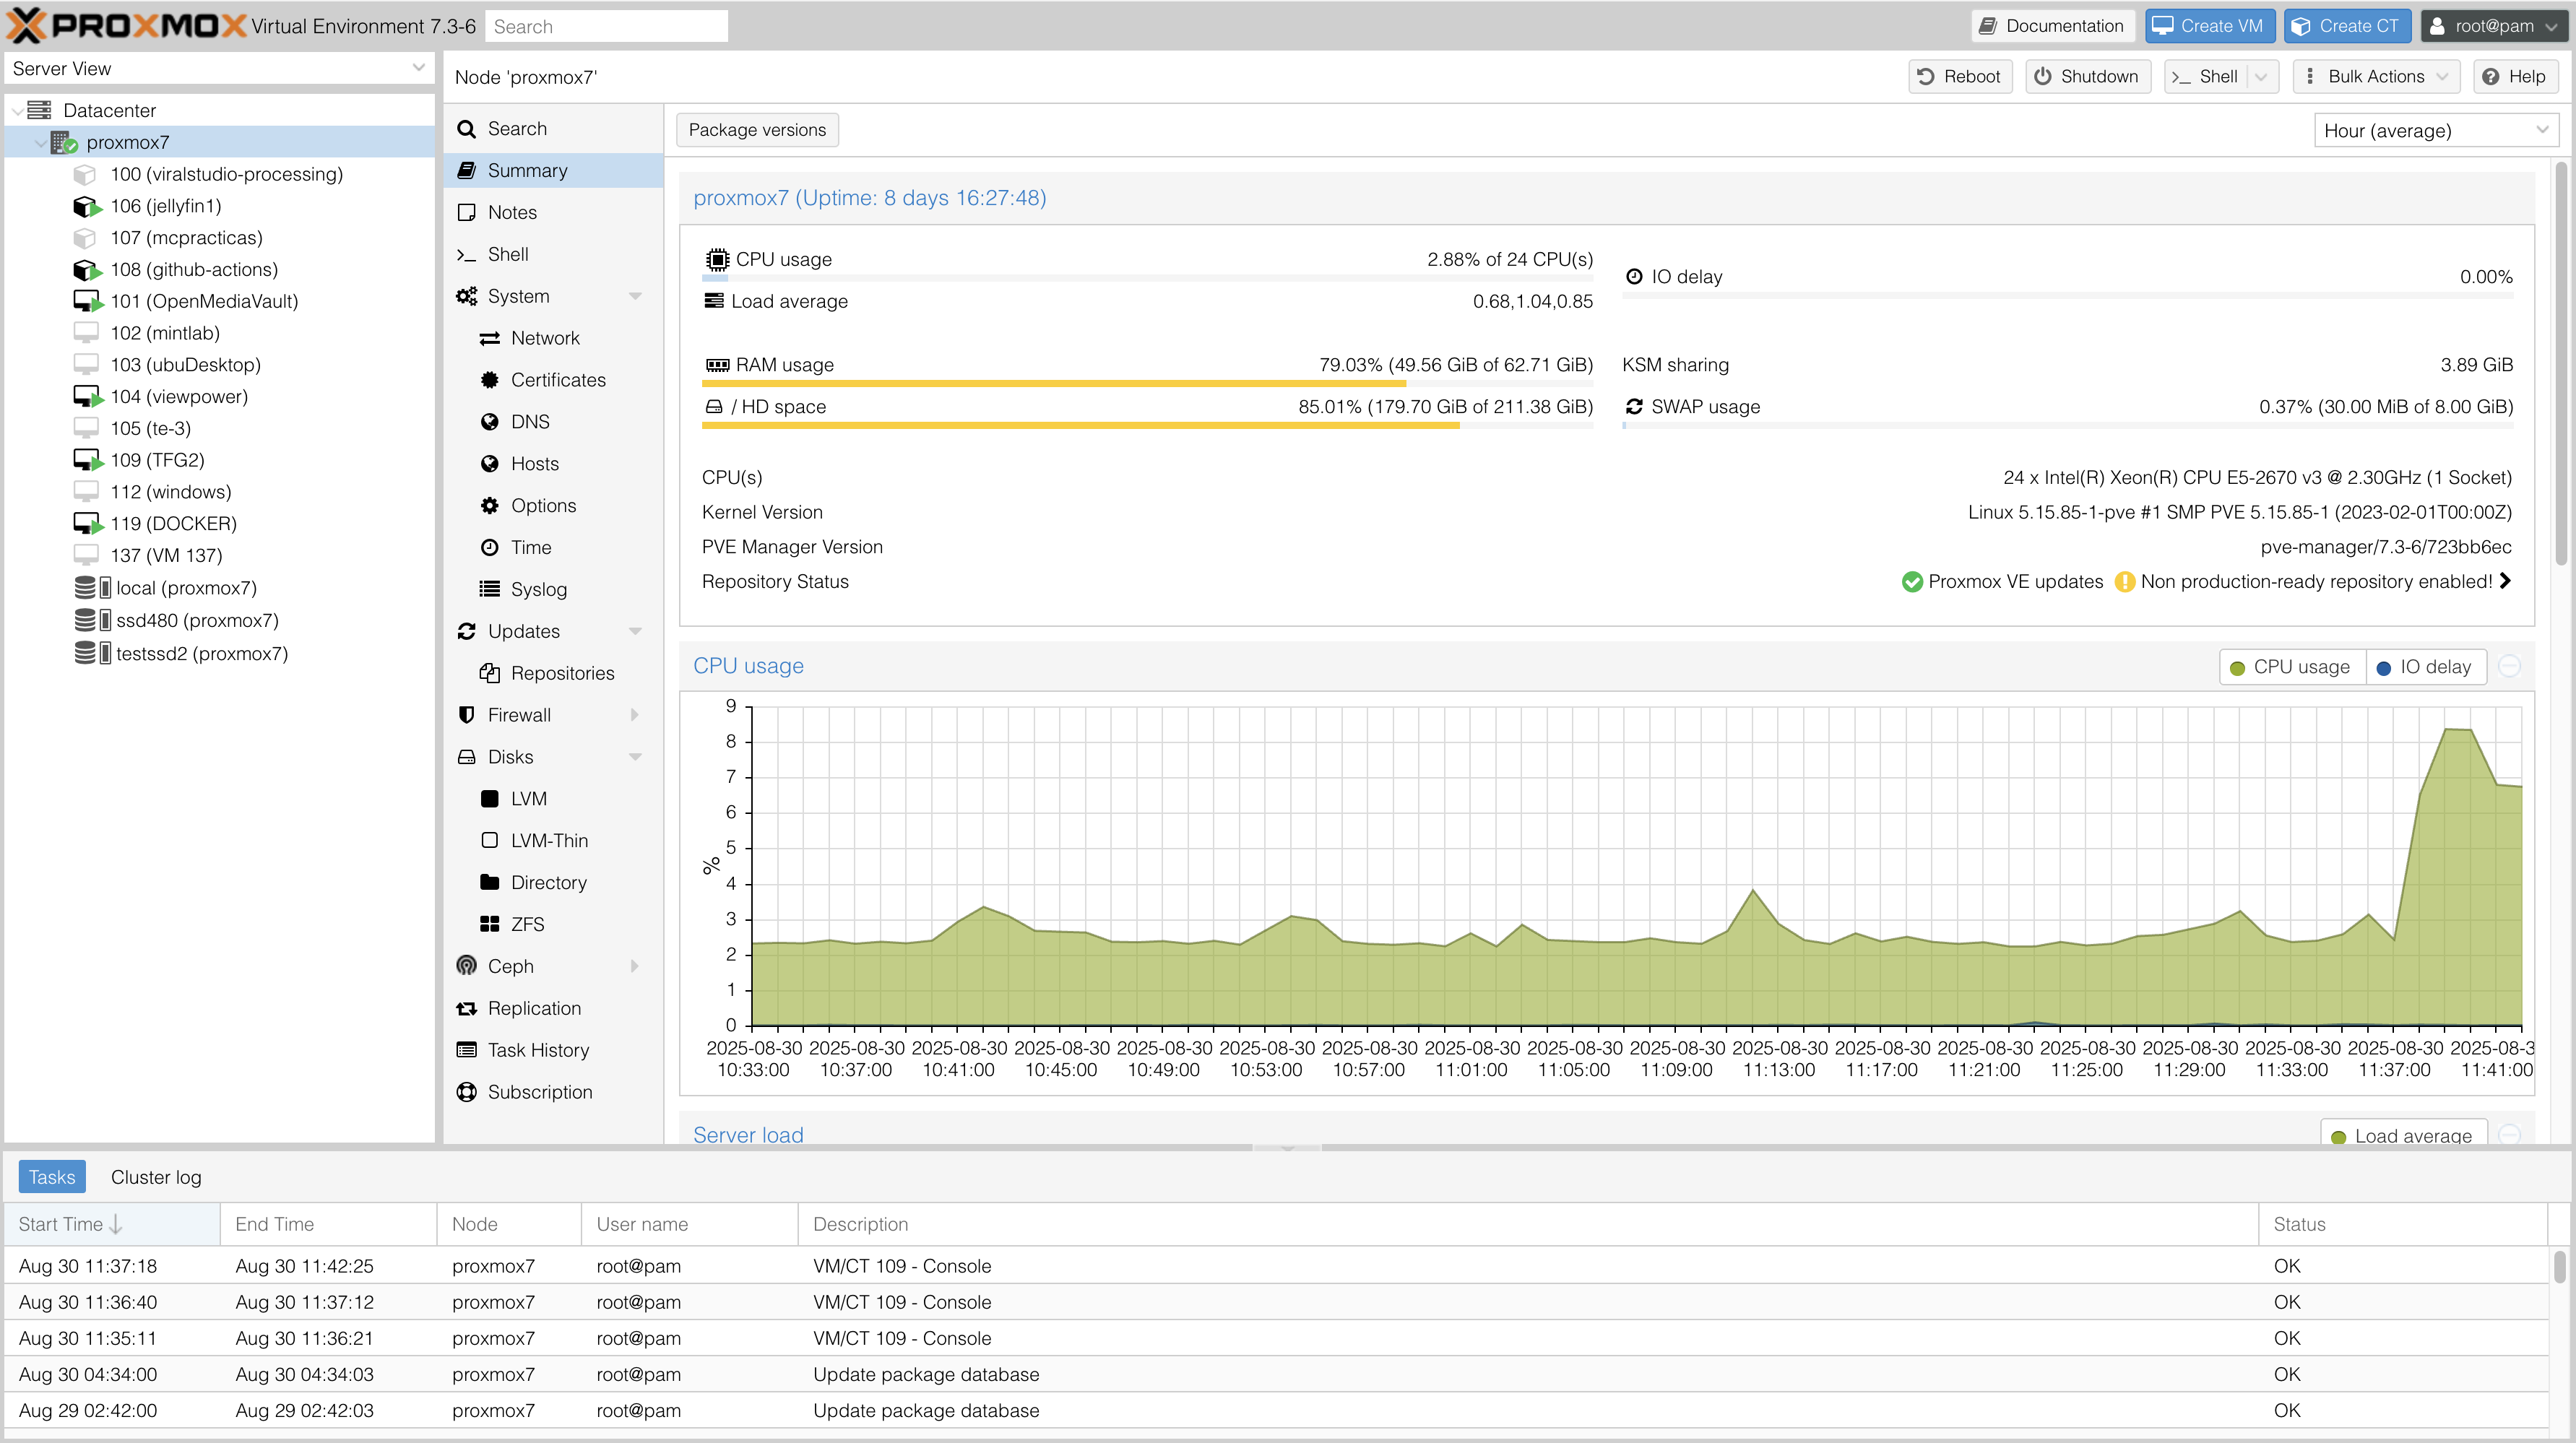
\includegraphics[width=1\textwidth]{imagenes/proxmox2.png}}
  %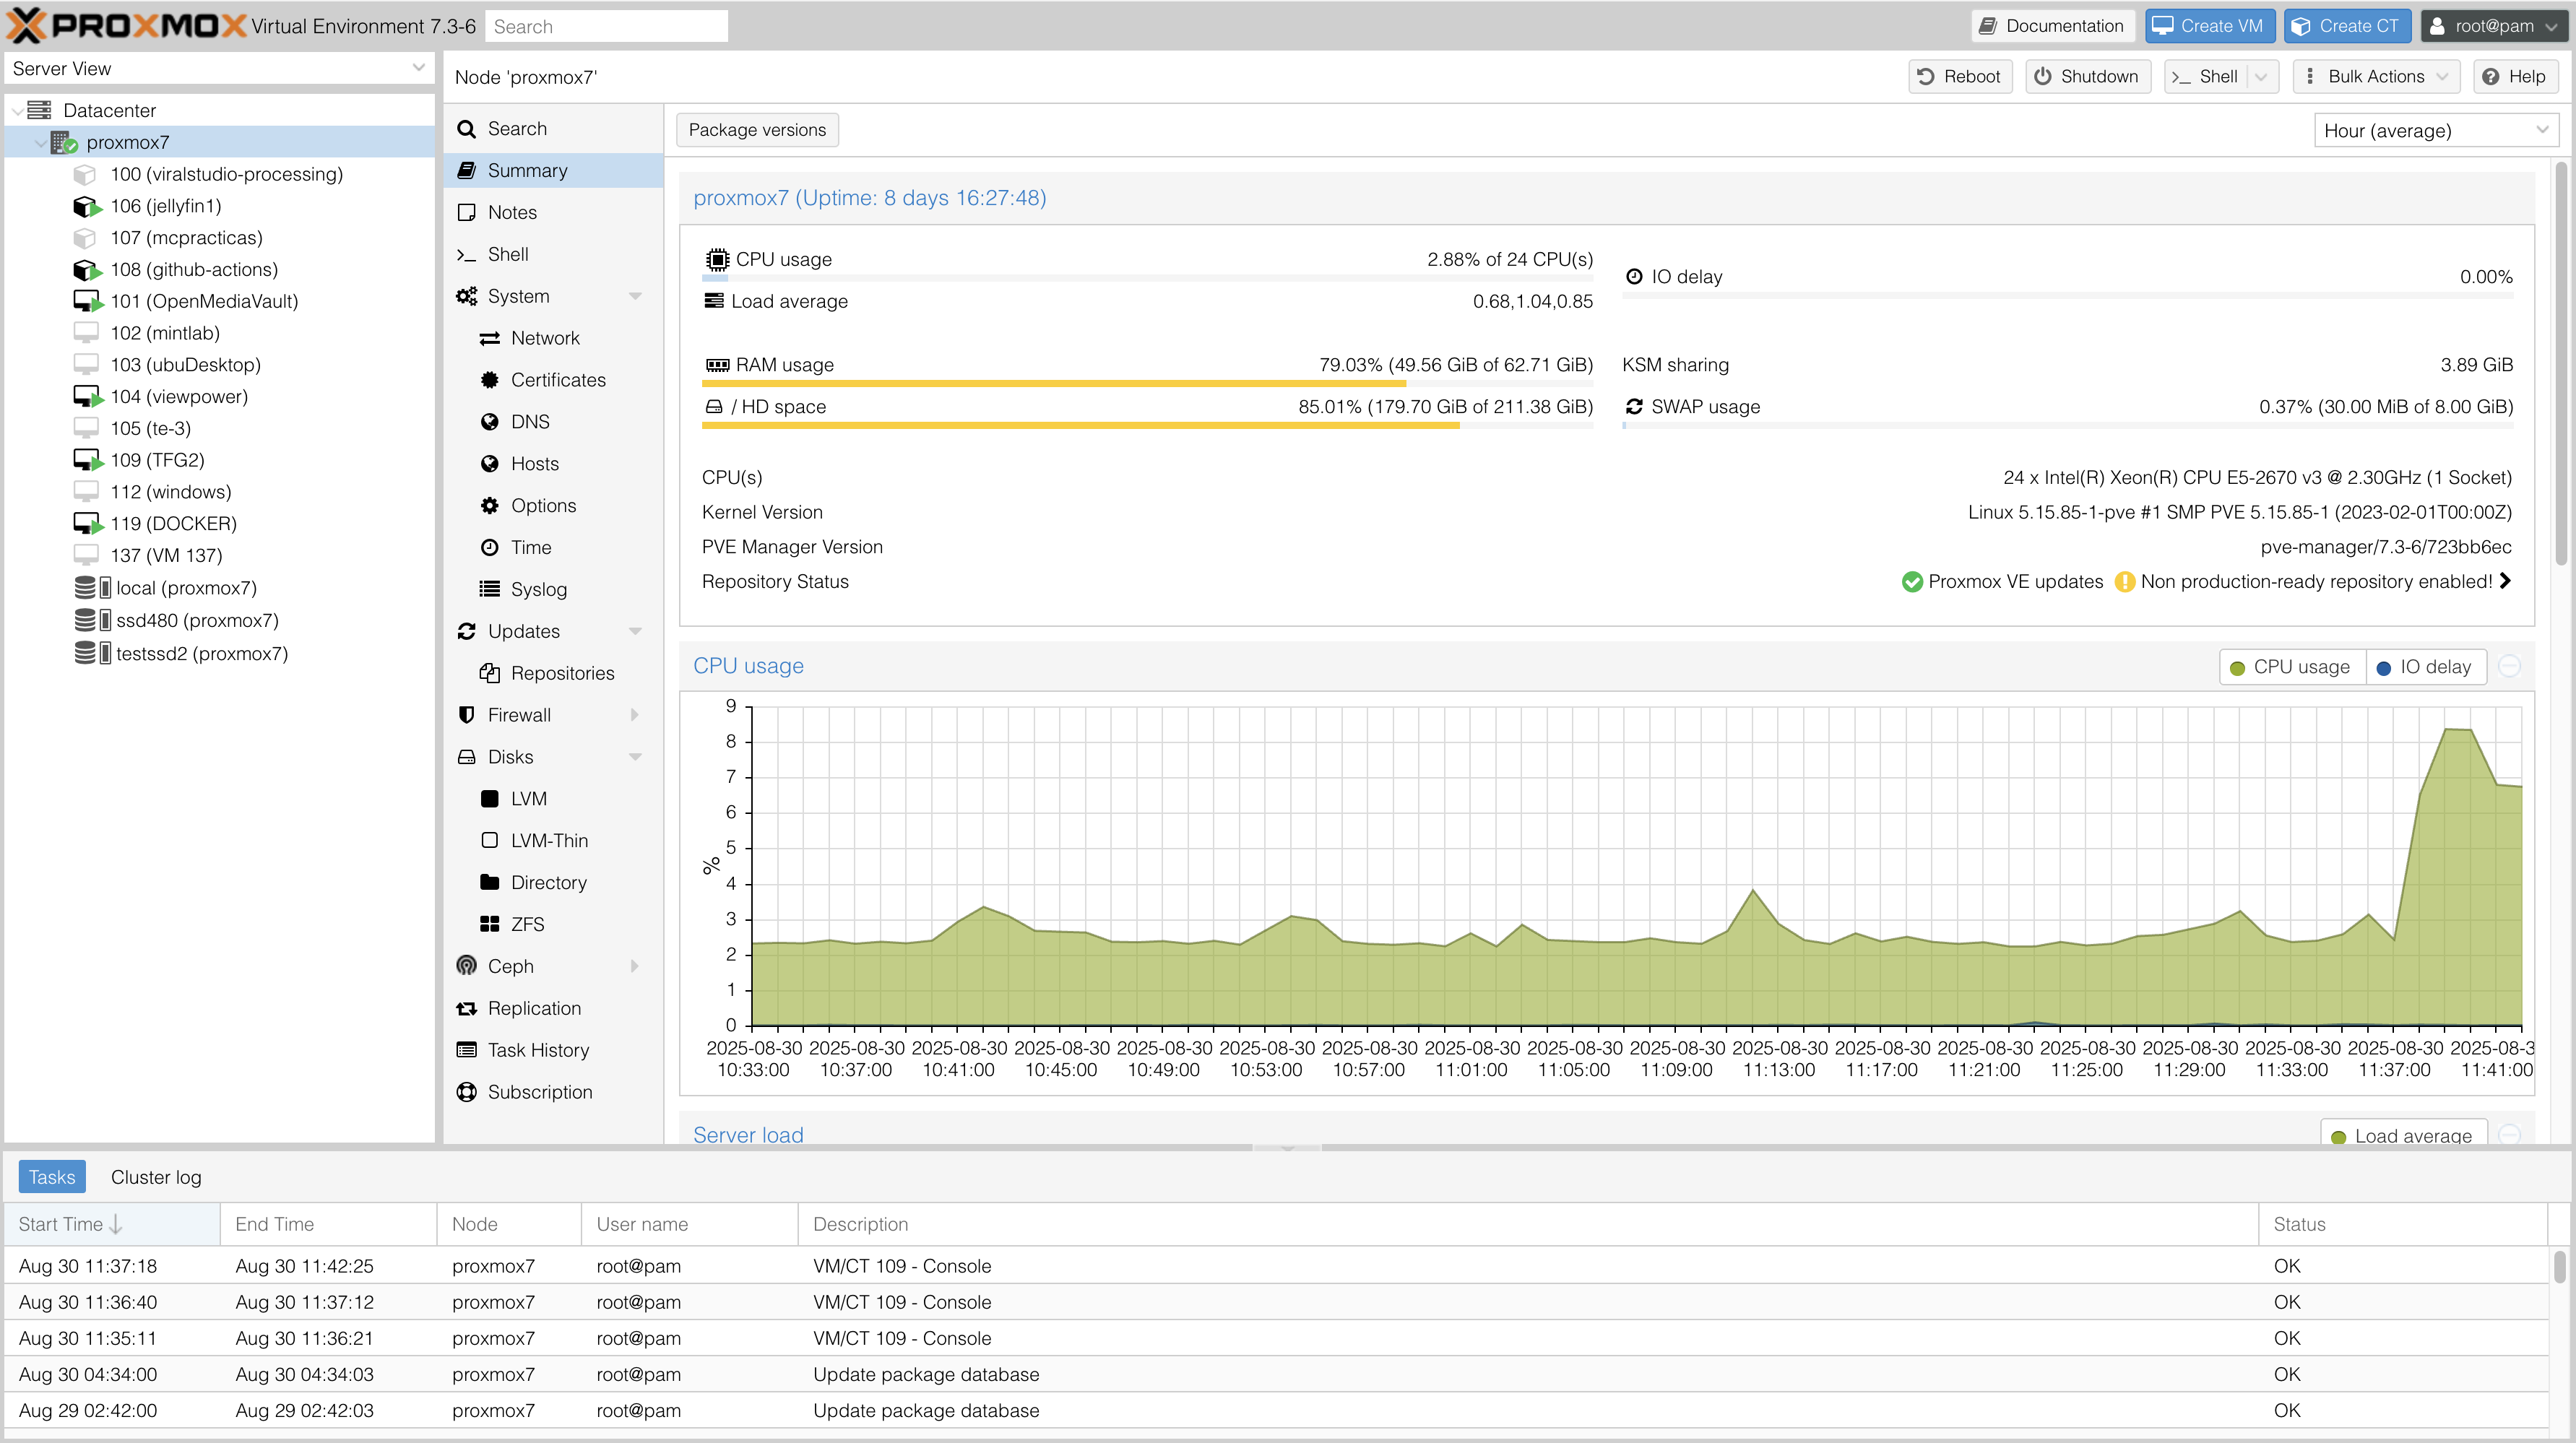
\includegraphics[width=1\textwidth]{imagenes/proxmox2.png}
  \caption{Captura de pantalla de la interfaz de Proxmox.}
  \label{fig:proxmox2}
\end{figure}



Se creó una máquina virtual con Ubuntu 24.04 Desktop como sistema operativo guest. Los recursos asignados a esta máquina virtual se fueron incrementando iterativamente según las necesidades observadas durante las pruebas de carga y la importación de datos. La configuración final establecida fue de 10 núcleos de CPU, 26 GB de memoria RAM y 128 GB de almacenamiento SSD, especificaciones que proporcionaron el rendimiento adecuado para gestionar tanto la base de datos MongoDB como la API.

Una vez que tanto la base de datos como la API funcionaban correctamente en el entorno local, era necesario desplegarlos para permitir el acceso público desde el frontend. Para esta tarea se utilizó Cloudflare Tunnels \cite{cloudflaretunnels}, que permite exponer servicios locales a Internet sin abrir puertos en el firewall ni configurar redirección de puertos. Cloudflare \cite{cloudflare} es una empresa que actúa como intermediario proporcionando servicios de CDN, DNS y seguridad web entre los usuarios finales y los servidores.

El despliegue se realizó mediante un contenedor Docker adicional que ejecuta el cliente \texttt{cloudflared}, estableciendo una conexión cifrada entre el servidor local y la infraestructura de Cloudflare. Esta implementación permite que la API sea accesible públicamente a través de un dominio o subdominio de nuestra elección, en nuestro caso \texttt{https://tfg-api.angeloyo.com}, proporcionando automáticamente certificados SSL/TLS, protección DDoS y optimizaciones de red.

Las principales ventajas de esta aproximación son su simplicidad y que mantiene el servidor completamente privado, ofreciendo una URL HTTPS estable consumible desde cualquier ubicación. Sin embargo, esta solución, aunque perfecta para el contexto de este TFG, no sería adecuada para entornos de producción profesionales donde se requerirían arquitecturas más robustas con balanceadores de carga, alta disponibilidad y redundancia geográfica.  


\begin{figure}[H]
  \centering
  \fbox{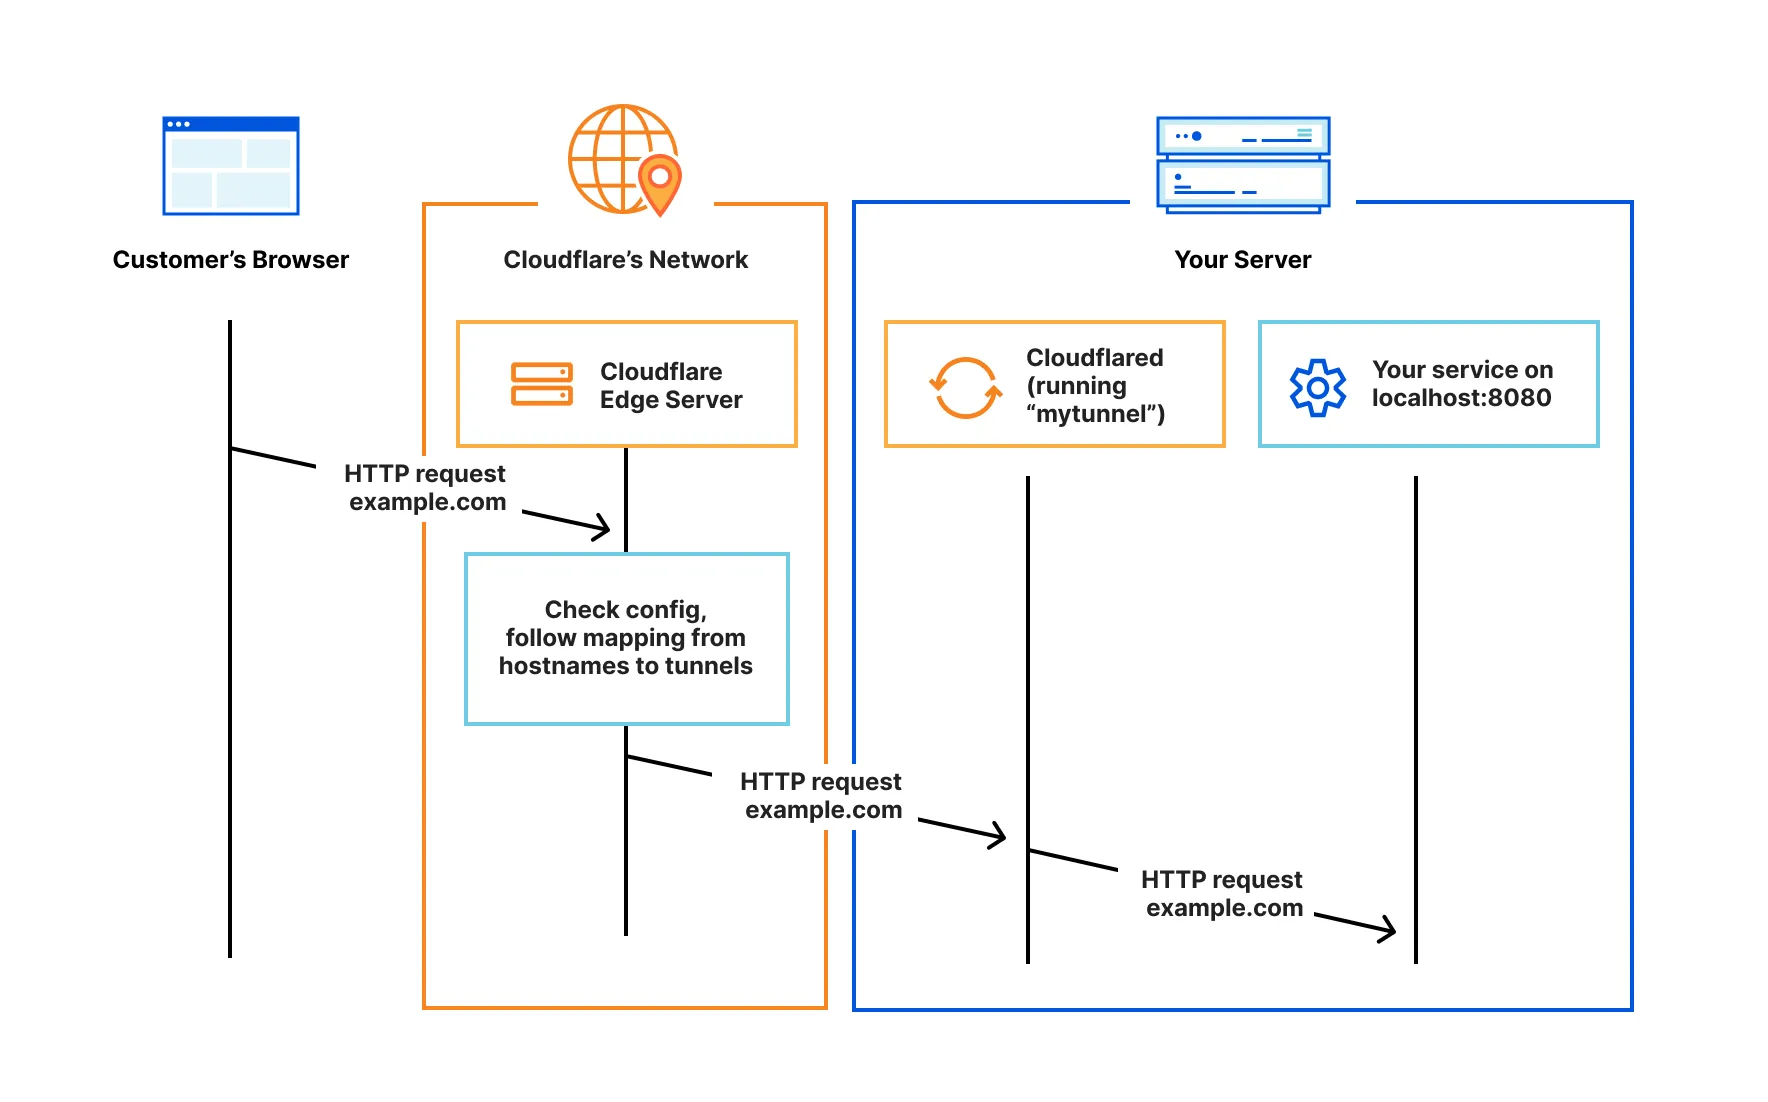
\includegraphics[width=1\textwidth]{imagenes/cloudflared.png}}
  %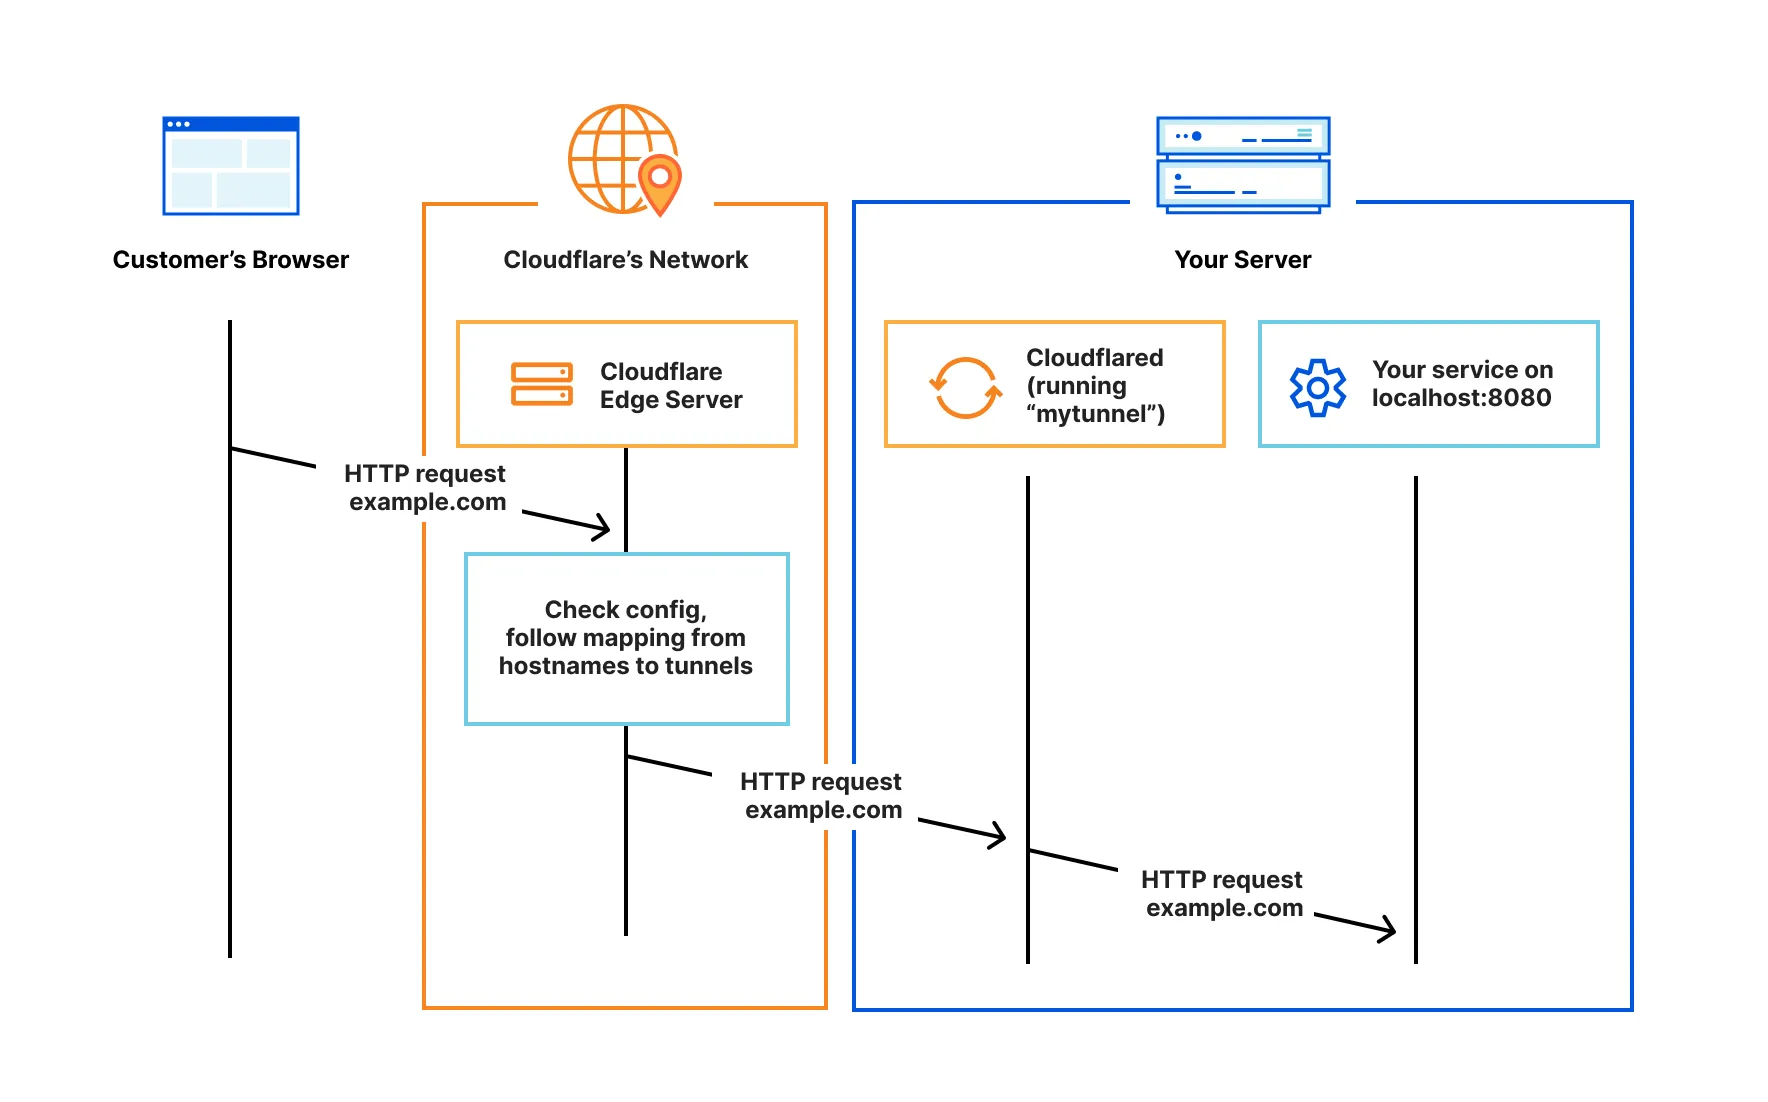
\includegraphics[width=1\textwidth]{imagenes/cloudflared.png}
  \caption{Esquema del funcionamiento de Cloudflare Tunnels \cite{cloudflaretunnels}.}
  \label{fig:cloudflared}
\end{figure}


\newpage
\section{Frontend}

%\subsection{Tecnologías}

El frontend está desarrollado utilizando Next.js 15 y TypeScript. Se aloja la web en Vercel por su extrema facilidad de uso, plan gratuito, auto-deploy desde GitHub, gran optimización y CDN global. La arquitectura se basa en componentes reutilizables y páginas especializadas que consumen la API del backend.



\subsection{Arquitectura de Componentes}

La estructura del frontend sigue las convenciones de Next.js con el nuevo App Router, organizando el código en:

\begin{itemize}
\item \textbf{Páginas:} Ubicadas en \texttt{src/app/}, incluyen la página principal, dashboard, búsqueda de pacientes, chat y visualizaciones específicas.
\item \textbf{Componentes:} En \texttt{src/components/}, contienen elementos reutilizables como el header, componentes de gráficos y elementos de UI.
\item \textbf{Hooks personalizados:} En \texttt{src/hooks/}, encapsulan lógica específica como el monitoreo de salud del backend.
\item \textbf{Tipos TypeScript:} En \texttt{src/types/}, definen las interfaces de datos para garantizar type safety.
\end{itemize}

Se utiliza Lucide React para iconografía consistente y Tailwind CSS para el diseño.

\subsection{Visualización de Datos}

Se ha implementado una estrategia progresiva para la visualización de datos, empleando dos librerías principales según la complejidad de cada caso. Para los gráficos más básicos se utiliza Observable Plot \cite{observableplot}, que ofrece soluciones preestablecidas y una integración sencilla. Cuando se requieren visualizaciones más complejas que demandan un control granular sobre el renderizado y la interactividad, se recurre a D3 \cite{d3}, también desarrollada por Observable, lo que permite adaptar los gráficos a necesidades avanzadas, sin salir del mismo ecosistema y estética.

Los componentes de visualización están diseñados como elementos autónomos que consumen datos de la API y manejan sus propios estados de carga y error. Esta aproximación facilita la reutilización y el testing individual de cada visualización.


\subsection{Páginas implementadas}

A continuación se detallan todas las páginas del Frontend que se han implementado. Se ha buscado una UI (User Interface) minimalista, limpia, sencilla y moderna.

\subsubsection{Página principal}

La página principal o ``home'' se ha buscado que sea muy sencilla, sólo se muestra el nombre dado a la plataforma, MIMIC-IV Analytics, junto a un pequeño subtítulo. 


\begin{figure}[H]
  \centering
  \fbox{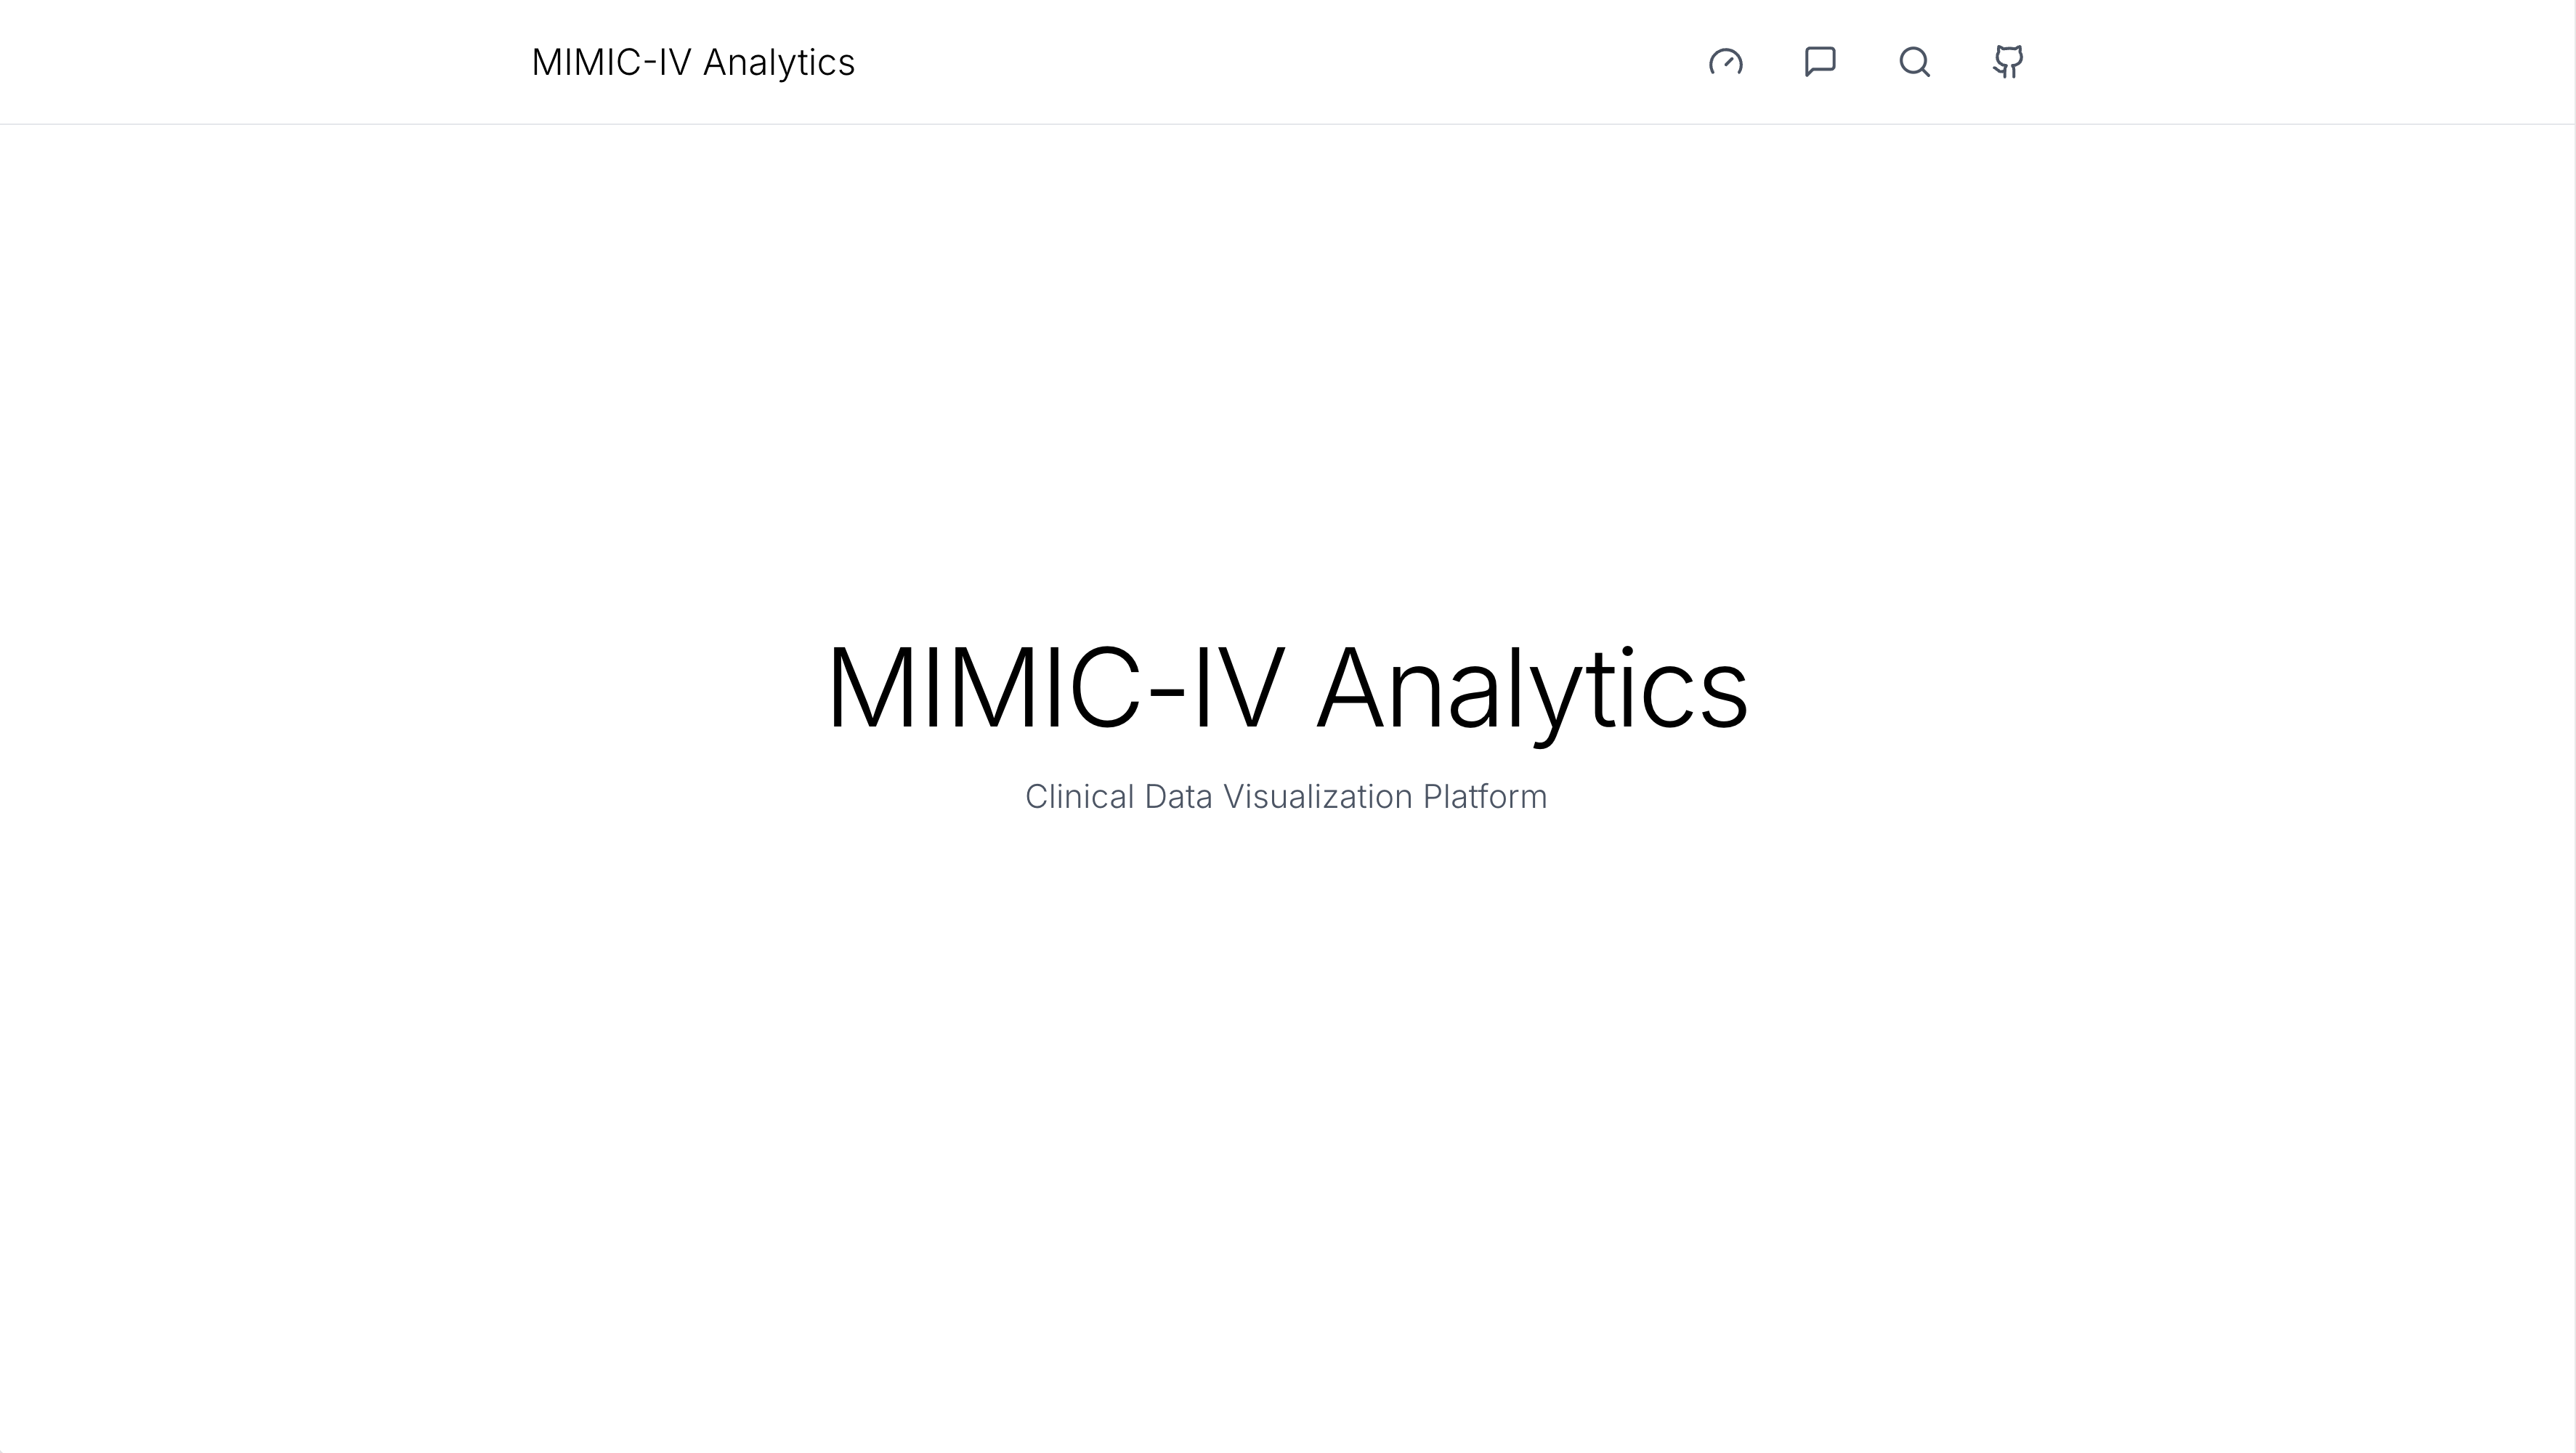
\includegraphics[width=1\textwidth]{imagenes/home.png}}
  \caption{Captura de pantalla de la página principal.}
  \label{fig:home}
\end{figure}


\subsubsection{Página del dashboard}

El objetivo de esta página es ofrecer al usuario una visión clara y accesible de las estadísticas más relevantes de la base de datos, seleccionadas por su importancia clínica. Para facilitar la interpretación y mejorar la experiencia de usuario, toda la información de MIMIC-IV se ha organizado en cinco grandes categorías: Demográficos y Admisiones, Cuidados Intensivos, Laboratorio y Medicamentos, Diagnósticos y Procedimientos, y Flujos Hospitalarios. En cada una de estas categorías se presentan tres indicadores estadísticos destacados, junto con enlaces a las visualizaciones asociadas. En total, se han implementado seis visualizaciones: dos para la categoría de Demográficos y Admisiones, y una para cada una de las categorías restantes.

En un entorno médico real e ideal, estos datos se actualizarían dinámicamente, permitiendo monitorizar de un vistazo los principales KPIs (Key Performance Indicators) y facilitando la toma de decisiones. Esta página sienta las bases para desarrollos futuros, en los que los profesionales sanitarios podrían filtrar los datos por periodos de tiempo, realizar comparativas o explorar tendencias, obteniendo así información relevante y actualizada sobre el estado del hospital. 


\begin{figure}[H]
  \centering
  \fbox{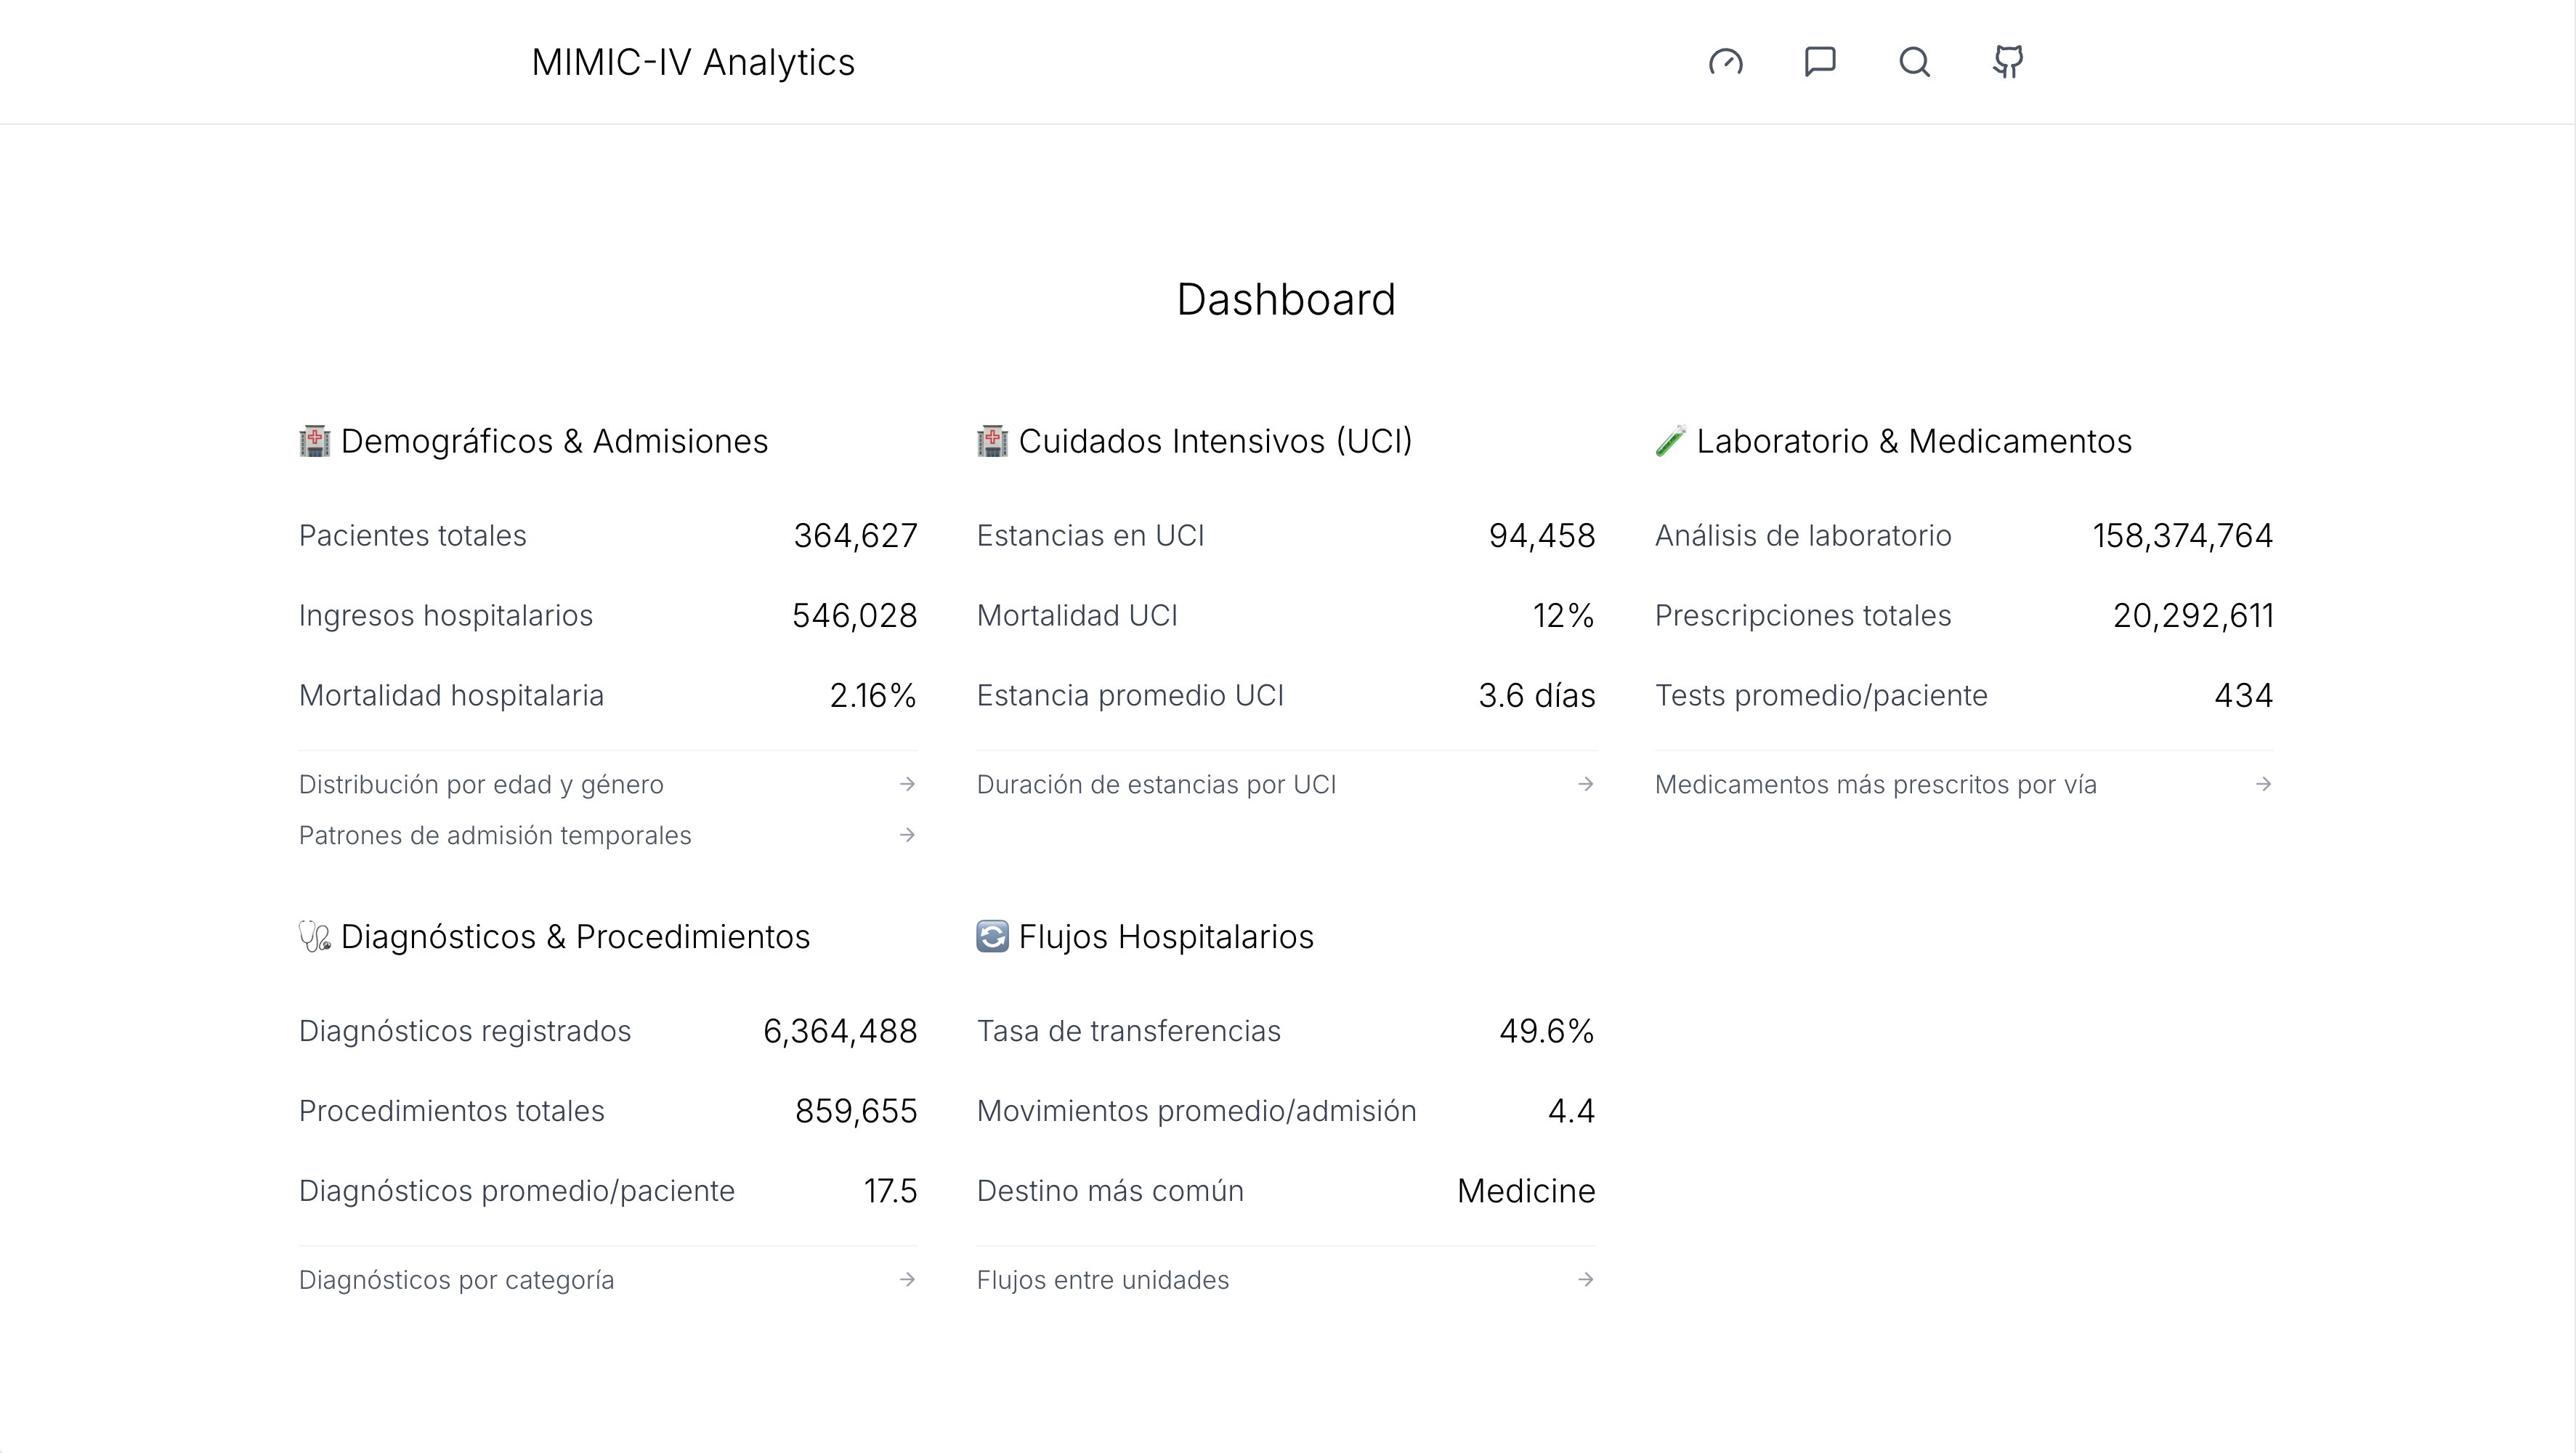
\includegraphics[width=1\textwidth]{imagenes/dash.png}}
  \caption{Captura de pantalla de la página del dashboard.}
  \label{fig:dash}
\end{figure}

\subsubsection{Página del chat}

Para la página del chat se sigue con la estética visual minimalista ya establecida, y se implementa la conexión con el backend, que ejecuta toda la lógica de comunicación entre el LLM, la base de datos gracias al protocolo MCP, y el frontend.

\begin{figure}[H]
  \centering
  \fbox{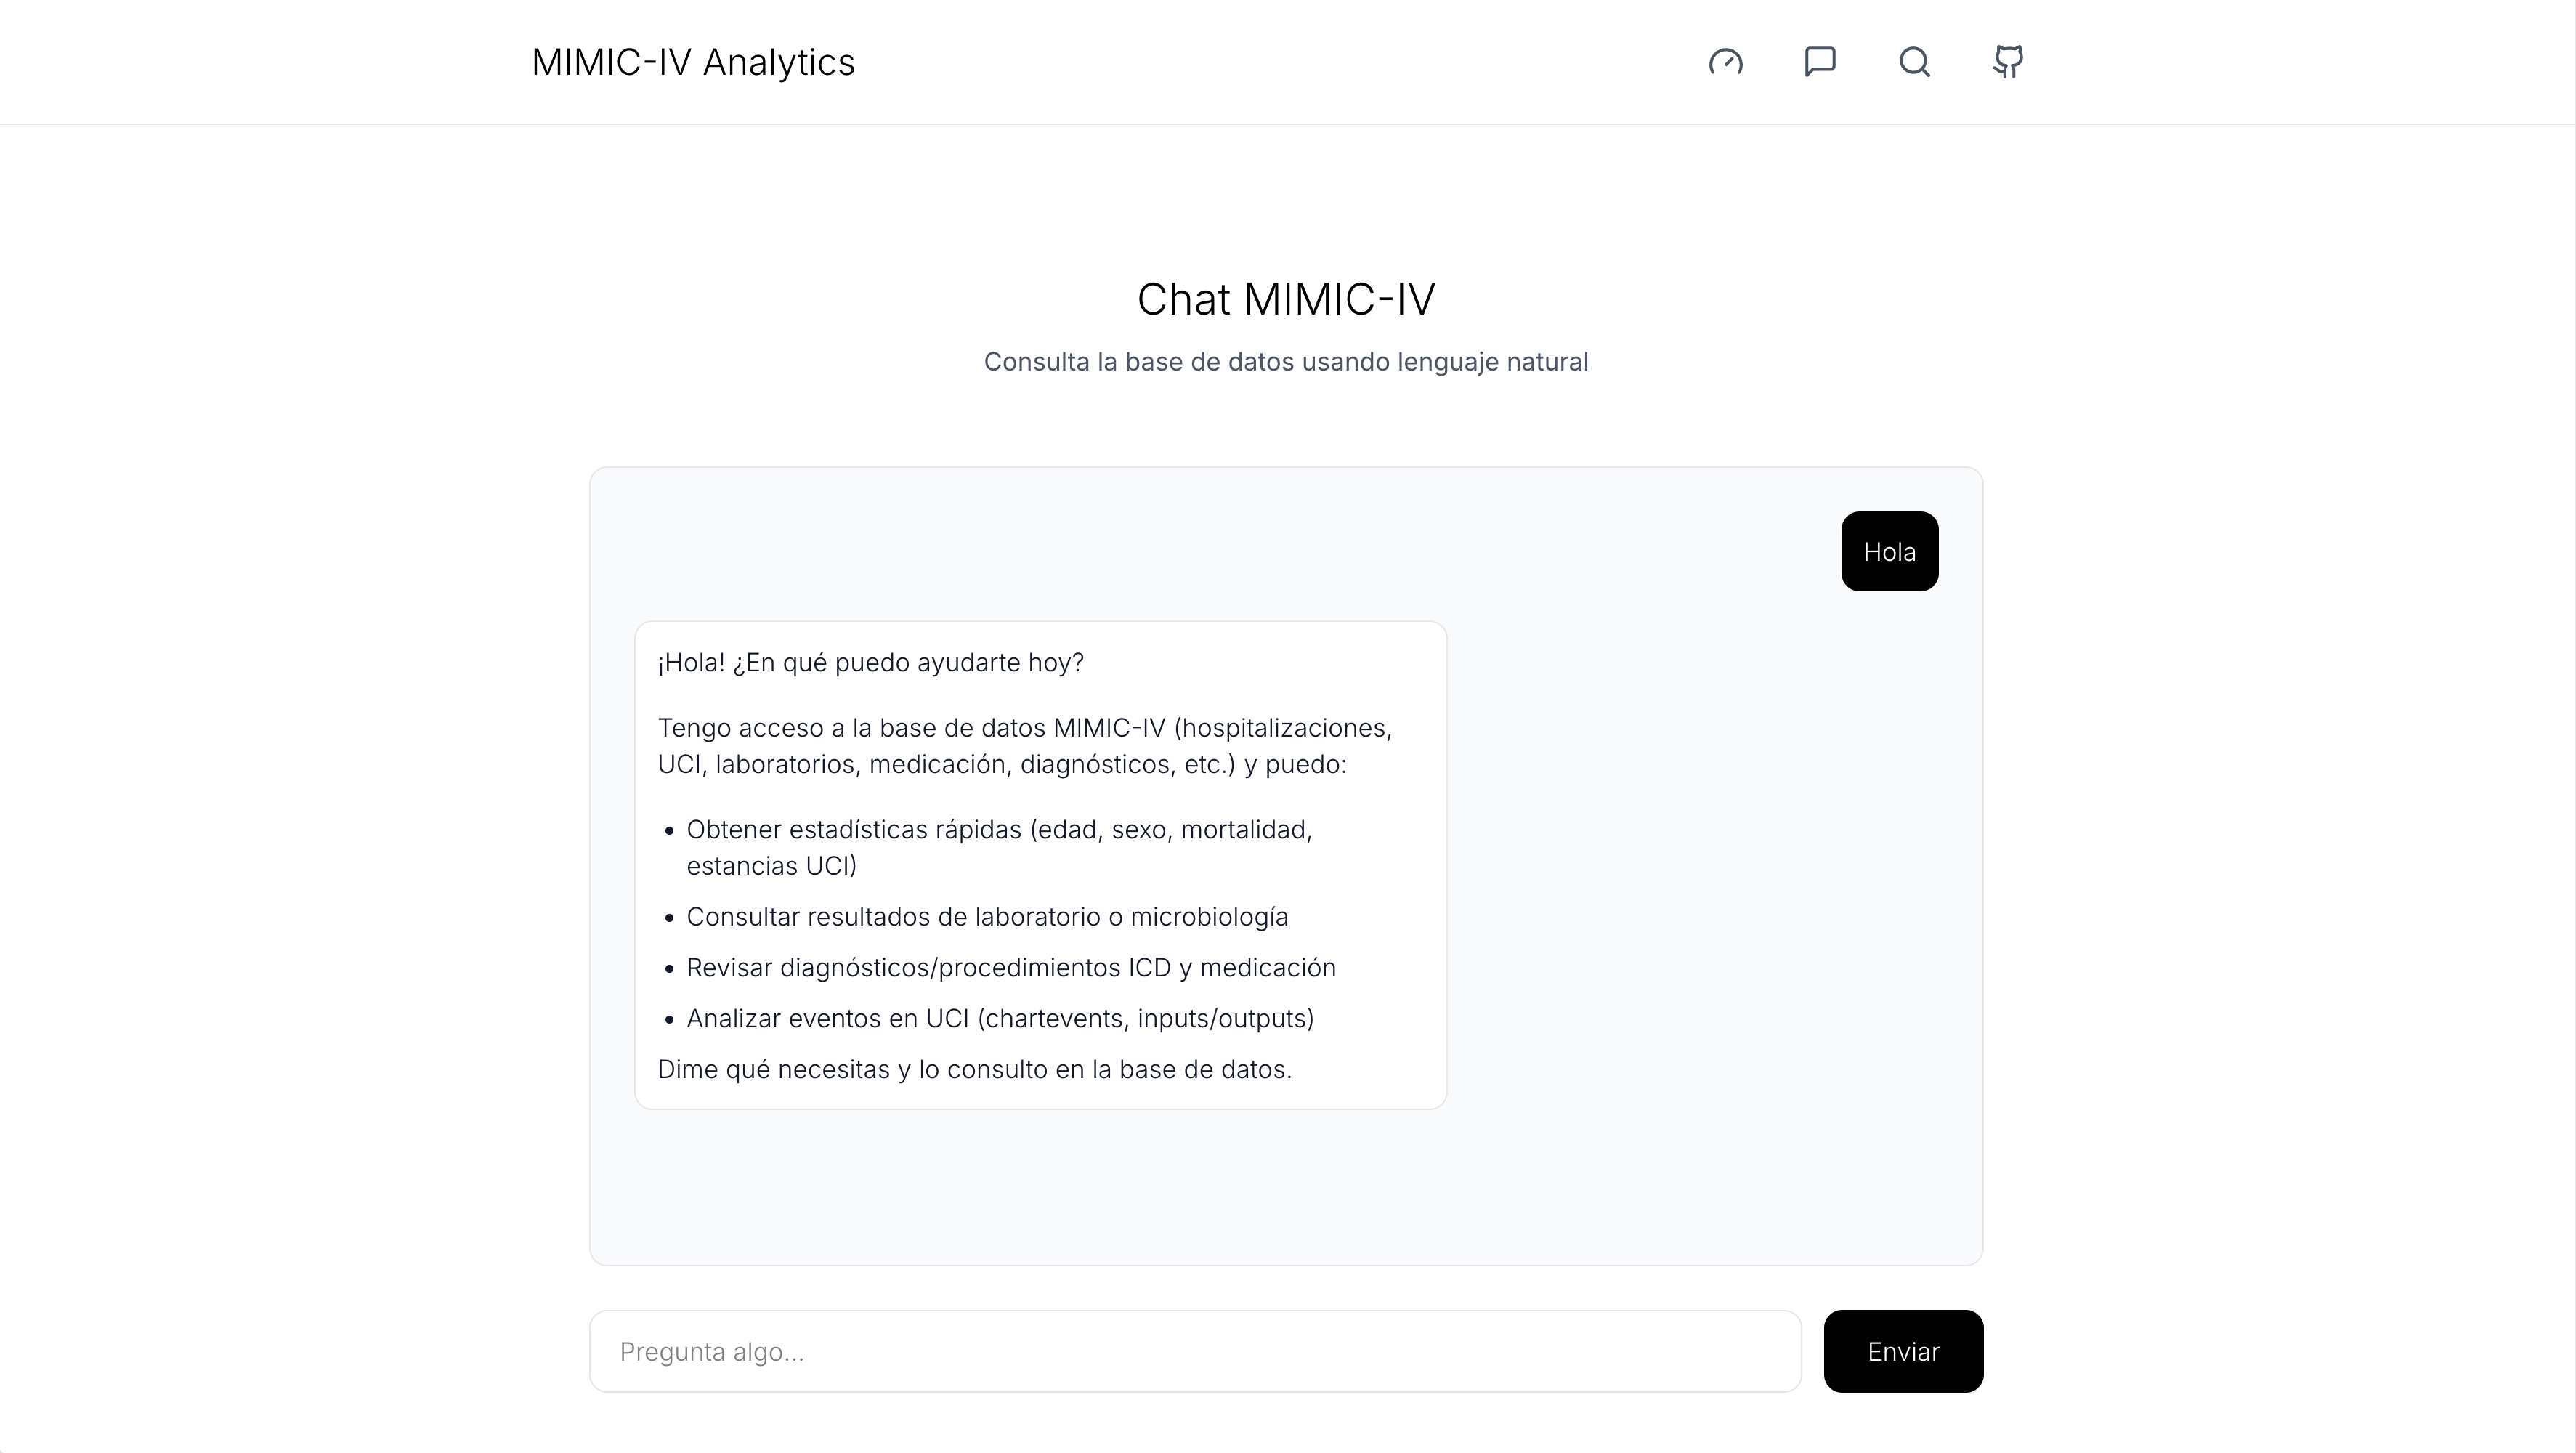
\includegraphics[width=1\textwidth]{imagenes/chat.png}}
  \caption{Captura de pantalla de la página del chat.}
  \label{fig:chat}
\end{figure}

\subsubsection{Página de búsqueda de pacientes}

Esta sencilla página nos permite comprobar la existencia de un paciente mediante su identificador único, mediante llamadas al endpoint del backend \texttt{/api/patients/\$\{id\}/exists}, y si es así (obtenemos status code 200 OK) entonces redirigimos a la página individual del paciente \texttt{/patient/\$\{id\}}. 

\begin{figure}[H]
  \centering
  \fbox{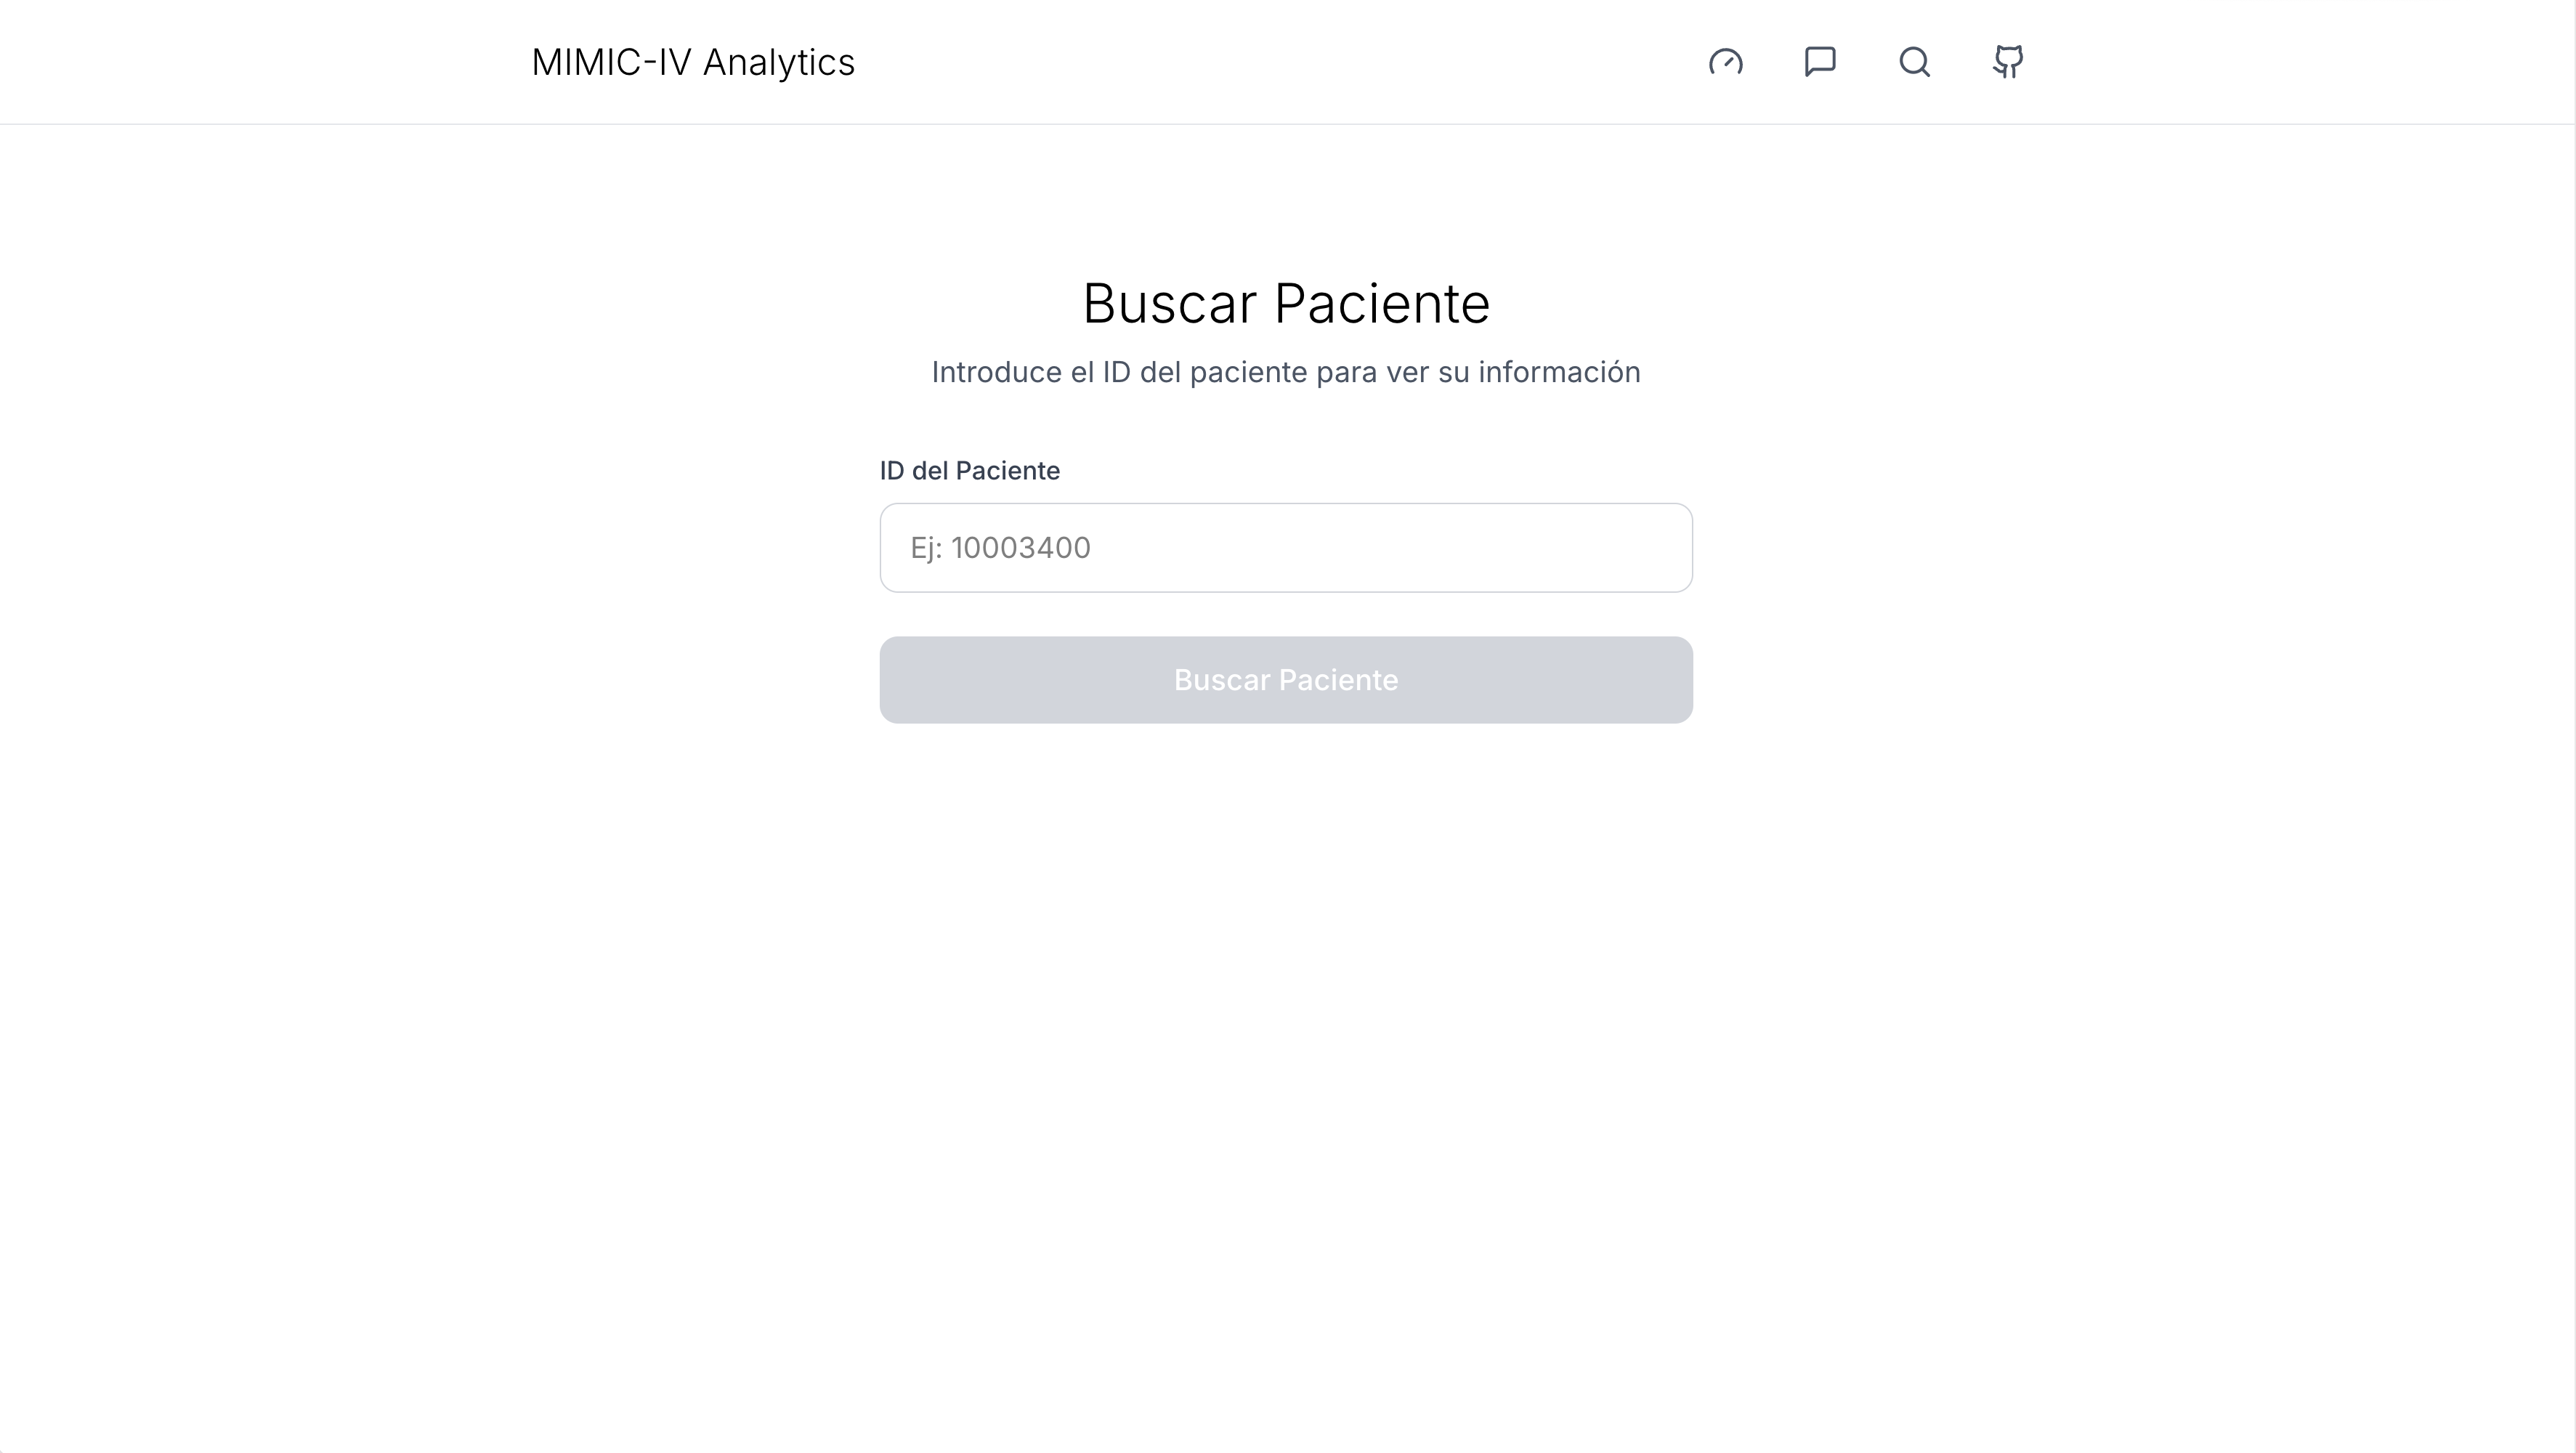
\includegraphics[width=1\textwidth]{imagenes/search.png}}
  \caption{Captura de pantalla de la página de búsqueda de pacientes.}
  \label{fig:search}
\end{figure}

\subsubsection{Página del paciente individual}

Al aterrizar en una de estas páginas, lo que hacemos es obtener el ID del paciente (\texttt{subject\_id}) de la URL, y lo envíamos al backend, a la ruta \texttt{/api/patients/\$\{id\}}. Este nos devuelve absolutamente toda la información relacionada con el paciente que necesitamos, por lo que puede tardar varios segundos en responder. Una vez con los datos, los mostramos de forma estructurada y visualmente agradable. A continuación se explican las tres secciones distintas en las que se ha organizado la información, las cuales han sido implementadas como componentes distintos que reciben los datos que necesitan de la página padre.

En primer lugar encontramos una sección con la información demográfica básica del paciente: género, edad, idioma, raza, etc. Implementado en el componente React \texttt{PatientBasicInfo}.

En segundo lugar, una sección en la que se muestra un resumen del paciente realizada con Inteligencia Artificial. El funcionamiento es el siguiente: una vez se reciben todos los datos del paciente y se carga la página, automáticamente el componente \texttt{PatientAISummary} llama a otro endpoint del backend \texttt{/api/summary/patient} y le envía todos los datos del paciente, para que se llame al LLM y se obtenga el resumen del historial. De esta forma, enviando los datos directamente y no el ID del paciente, nos ahorramos el tiempo de espera de volver a agregar toda información.

En tercer lugar tenemos el grueso de la información, en el componente \texttt{PatientAdmissions}. En el mediante desplegables, vemos un listado de todos los ingresos que ha tenido el paciente, junto a algunas estadísticas rápidas para ver a simple vista: número de días de duración de la hospitalización, número de diagnósticos asociados a la estancia, número de procedimientos, y número de tests de laboratorio. 

Al hacer click en el desplegable, podemos ver más información del ingreso, como las fechas exactas de entrada y salida, el tipo del seguro del paciente, a dónde se trasfirió despues, etc. Además, de nuevo, a forma de desplegables, podemos ver la información detallada de los diagnósticos, procedimientos, y tests de laboratorio.

En cuanto a los últimos, se ha implementado poder filtrar los tests según su categoría (Blood Gas, Hematology, Chemistry...) o bien verlos todos a la vez. De nuevo, se muestra el listado de los tests como un listado de elementos desplegables, búscando la limpieza visual al encapsular la información y visualizar sólo los datos que se quieren ver. Cuando se hace click en uno de los tests, si éste tiene dos o más ocurrencias, se mostrará una gráfica con la evolución temporal para dicha métrica. 


\begin{figure}[H]
  \centering
  \fbox{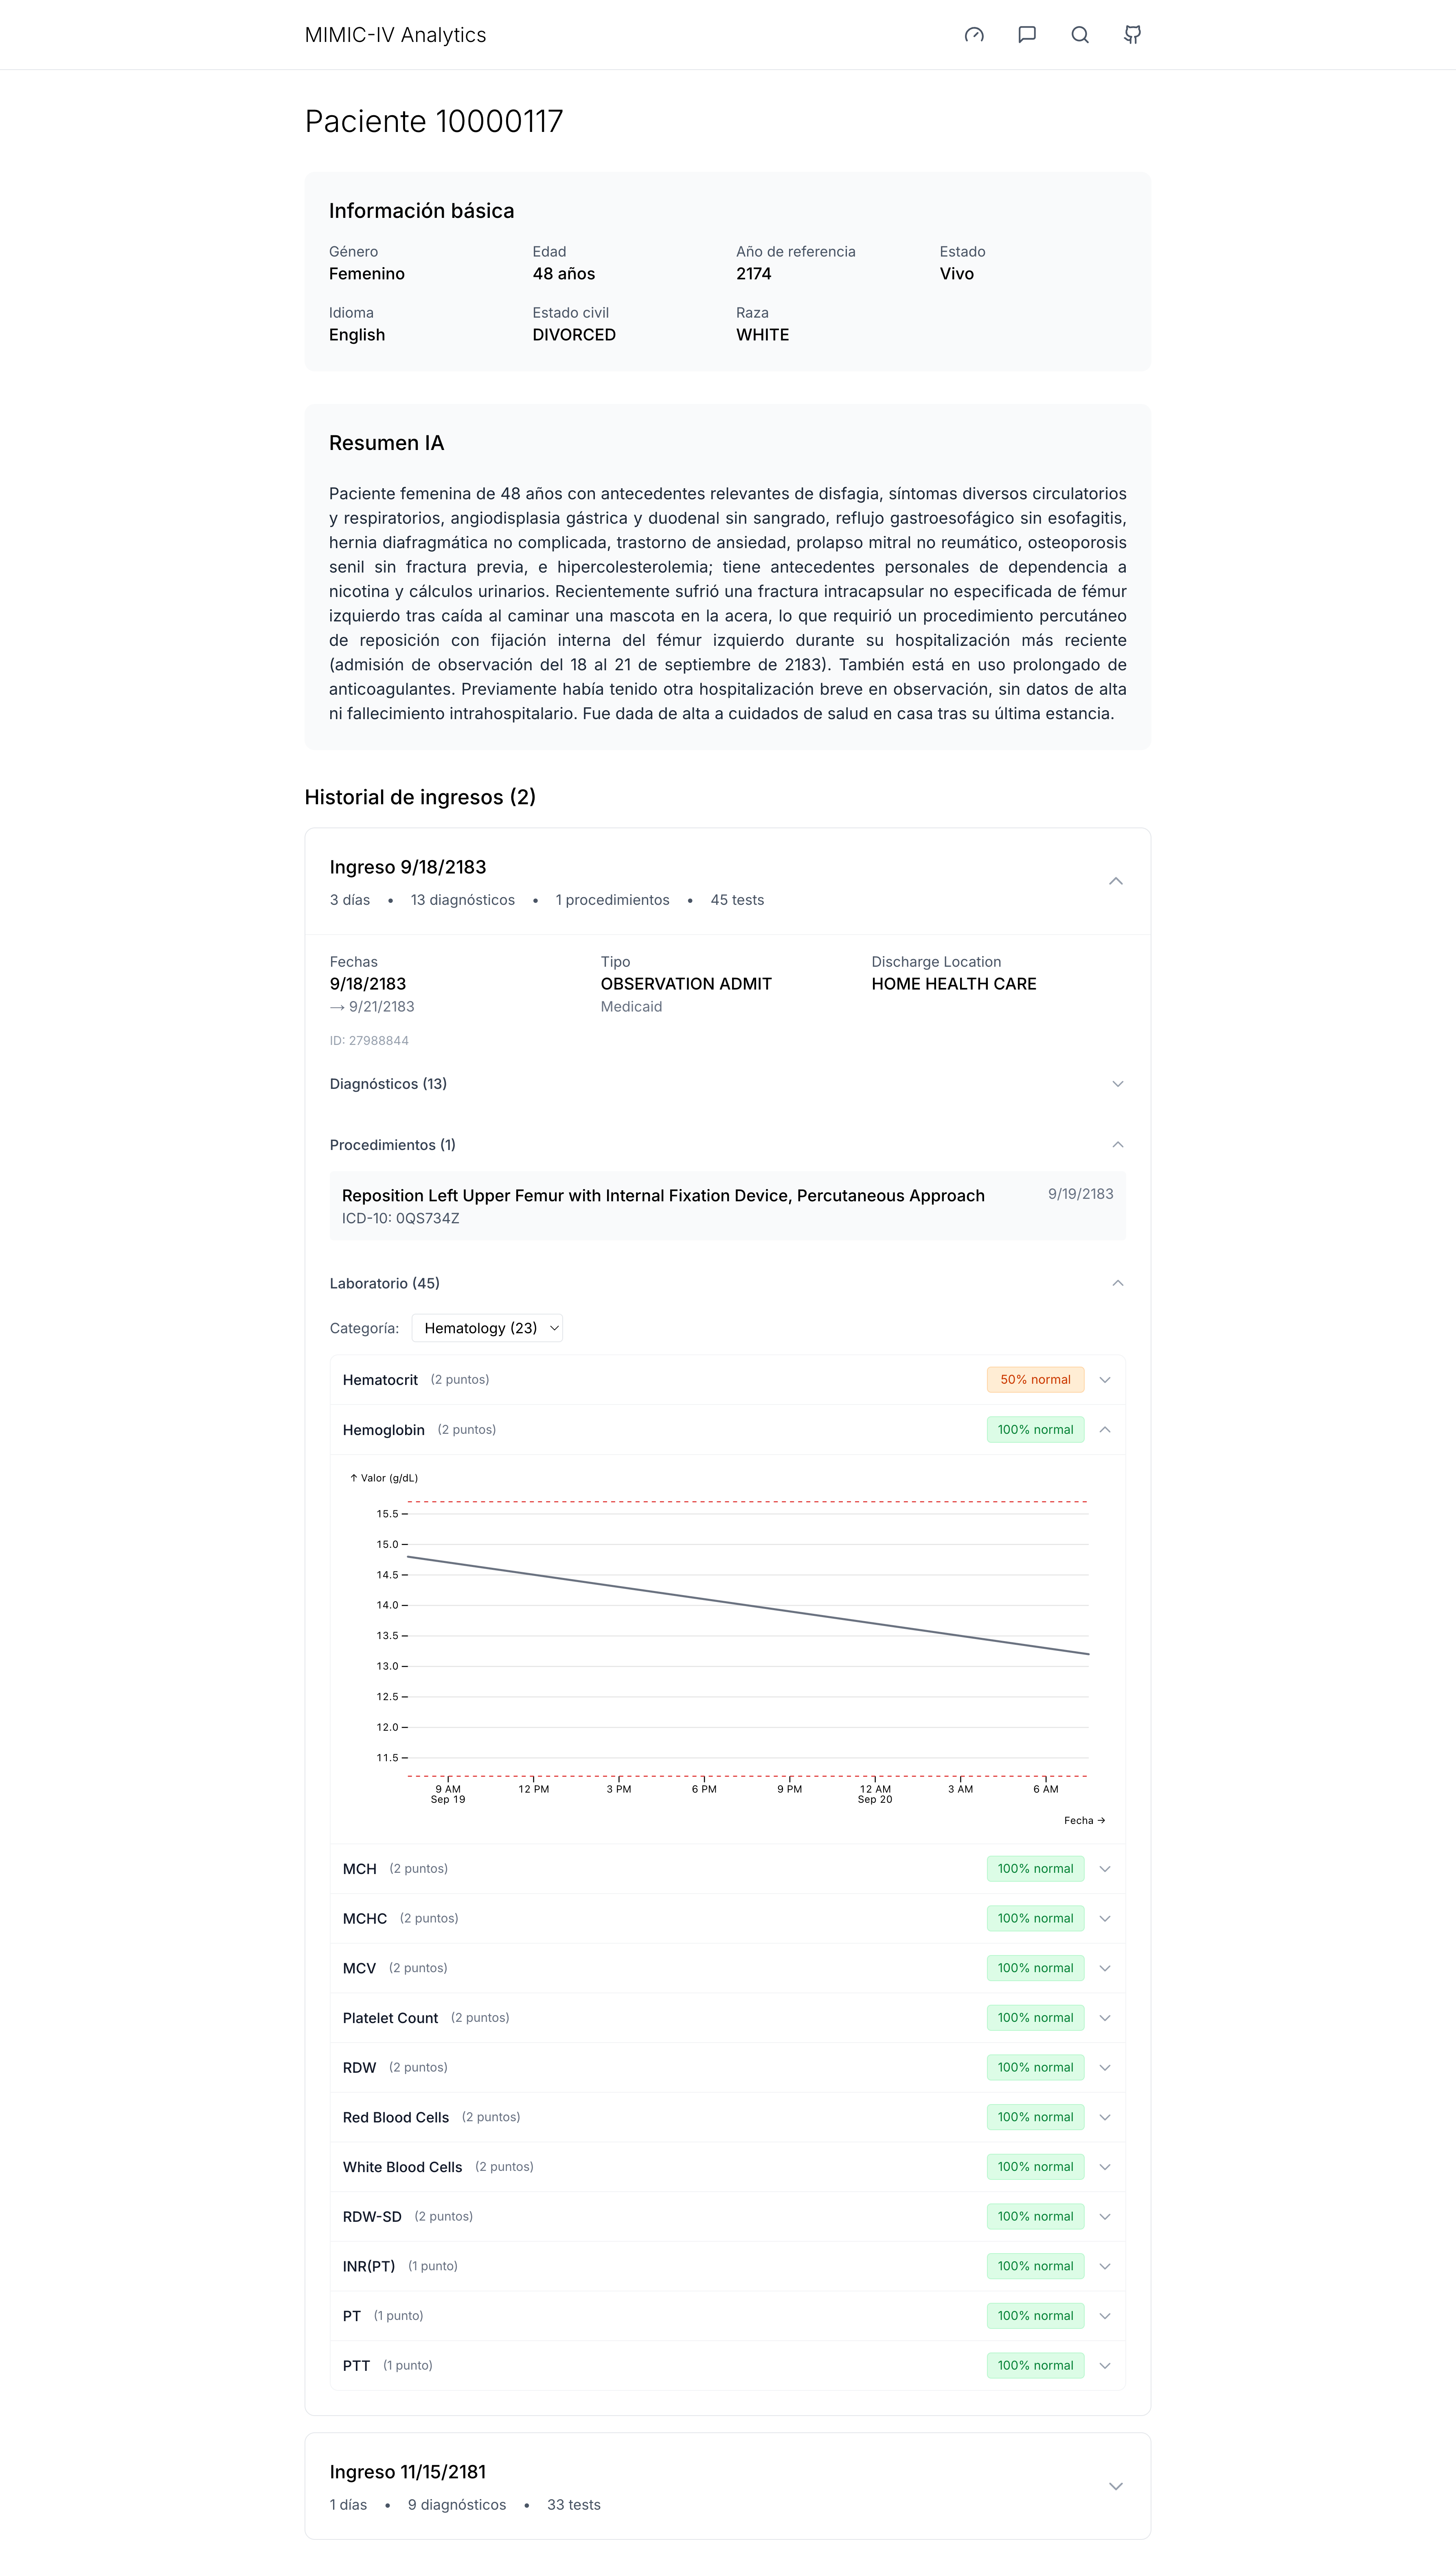
\includegraphics[width=0.9\textwidth]{imagenes/patient1.png}}
  \caption{Captura de pantalla de la página de búsqueda de pacientes.}
  \label{fig:search}
\end{figure}

%-----------------
\subsubsection{Página de gráfico: distribución por edad y género}

Ahora vamos a pasar a las visualizaciones de datos que se han implementado. El primer gráfico, realizado utilizando Observable Plot, es un Population Pyramid \cite{populationPyramid} de la distribución por edad y género, con dos variantes, una por rangos de edad, y la otra por edad específica.


\begin{figure}[H]
  \centering
  \fbox{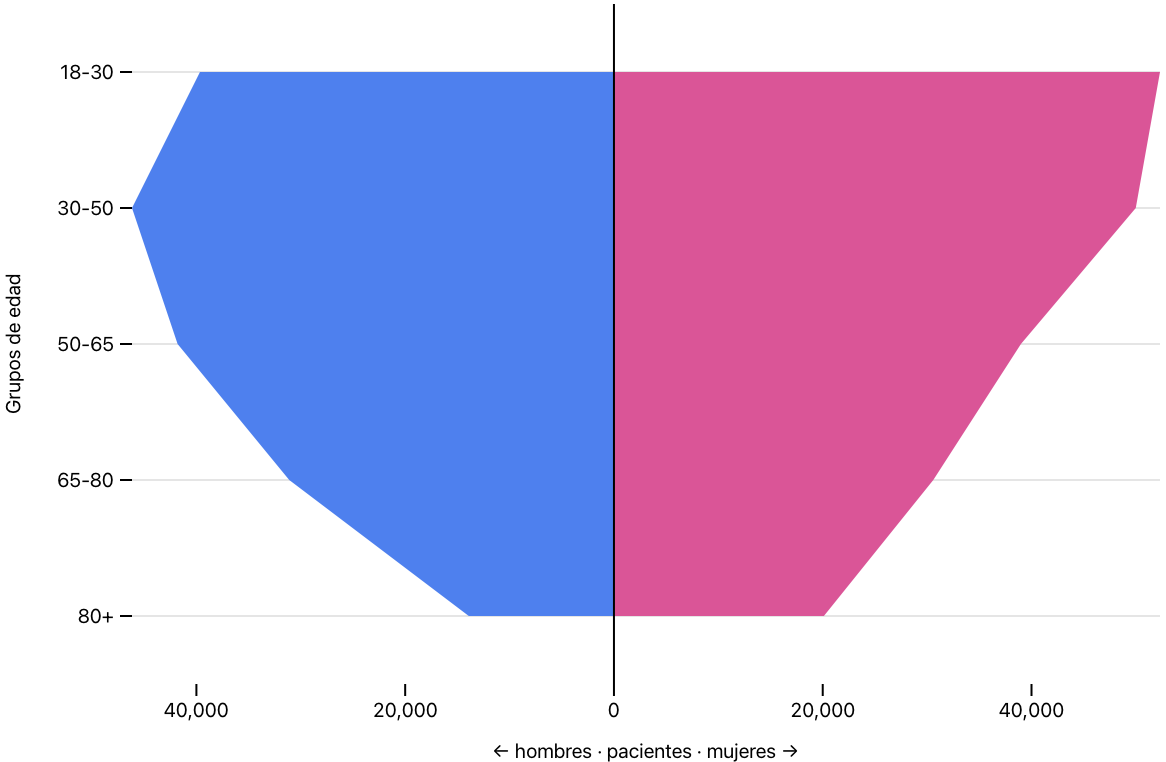
\includegraphics[width=0.65\textwidth]{imagenes/chart2.png}}
  %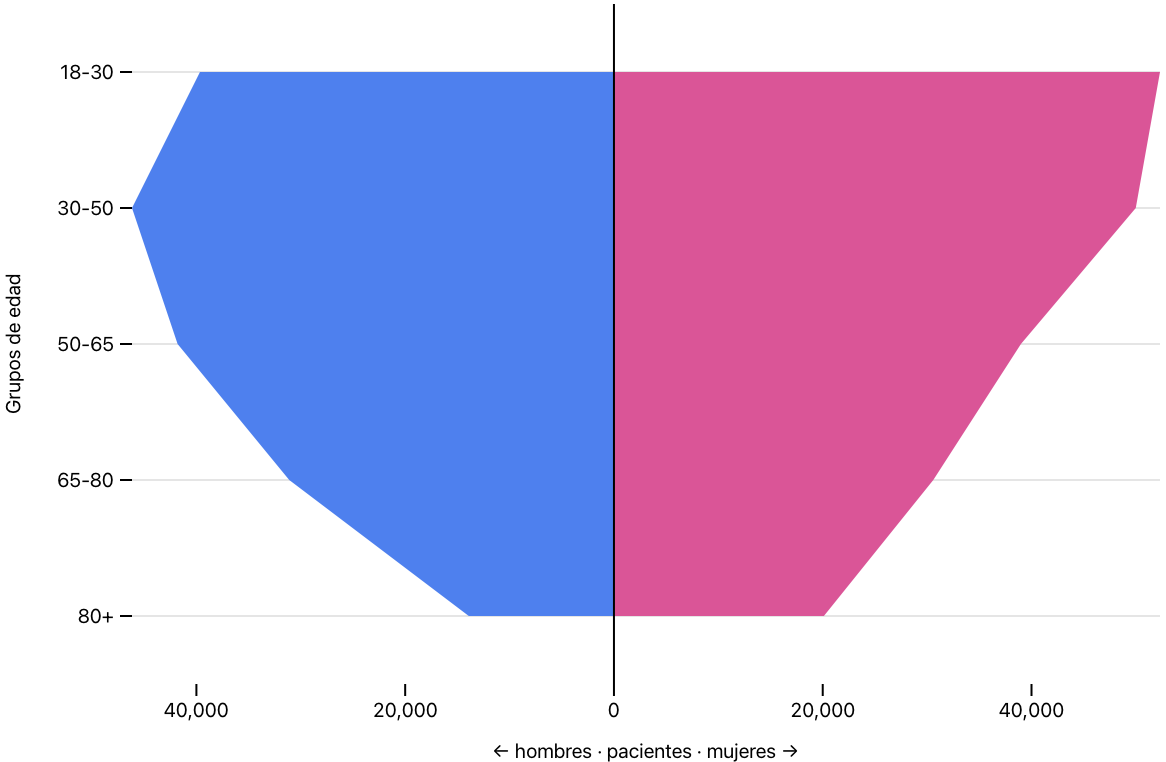
\includegraphics[width=0.65\textwidth]{imagenes/chart2.png}
  \caption{Distribución por edad y género (rangos de edad)}
  \label{fig:chart2}
\end{figure}

\begin{figure}[H]
  \centering
  \fbox{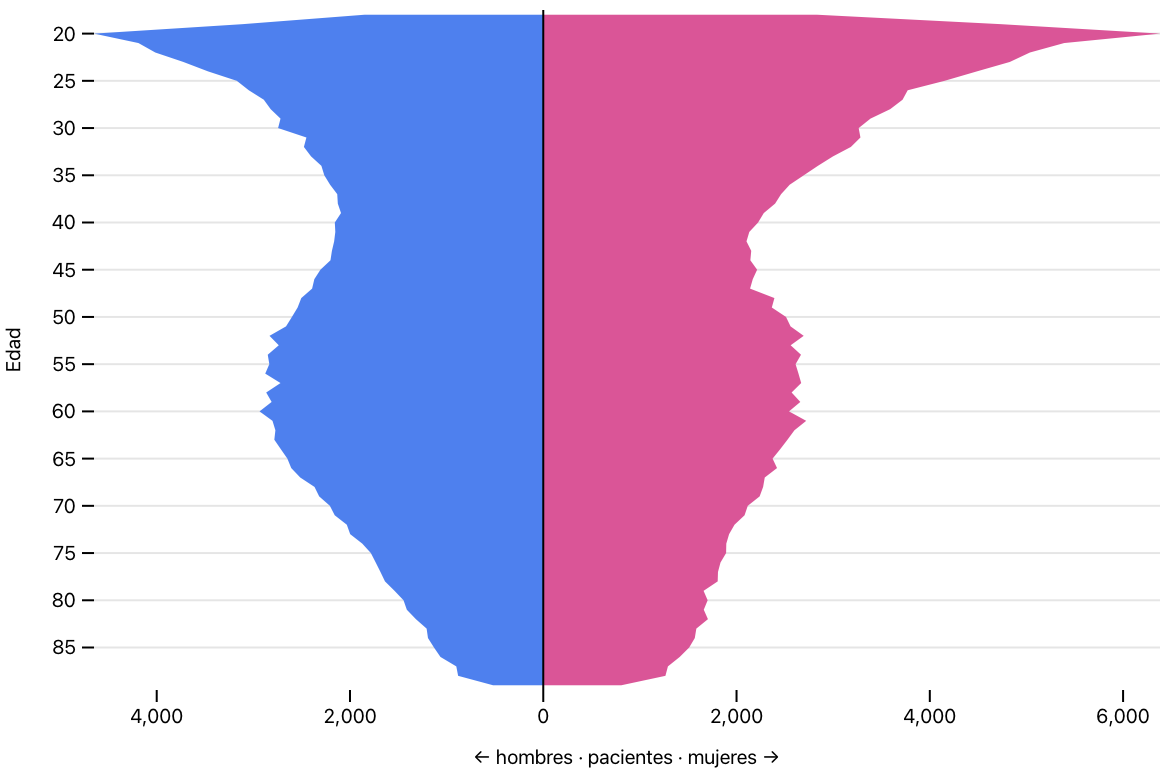
\includegraphics[width=0.65\textwidth]{imagenes/chart3.png}}
  %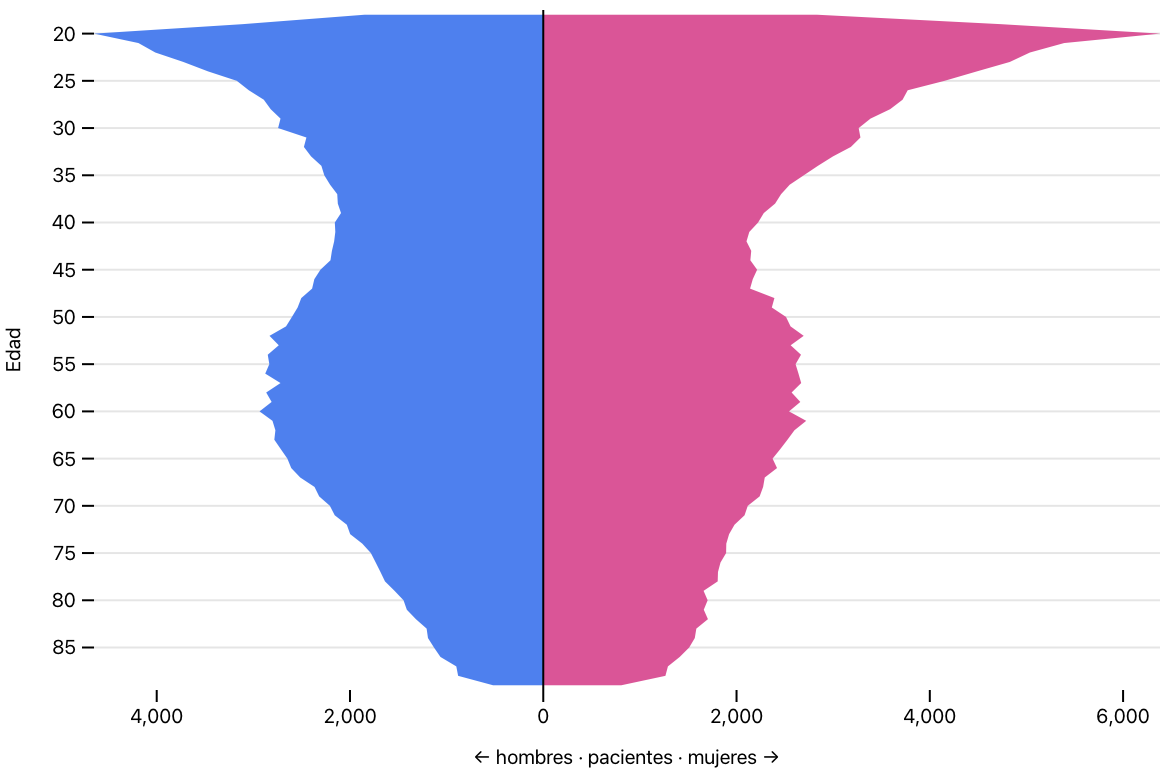
\includegraphics[width=0.65\textwidth]{imagenes/chart3.png}
  \caption{Distribución por edad y género}
  \label{fig:chart3}
\end{figure}


%-----------------
\subsubsection{Página de gráfico: heatmap de ingresos}

El segundo gráfico, también desarrollado con Observable Plot, consiste en un heatmap\cite{heatmap} que representa la cantidad de ingresos hospitalarios en función de la hora y la fecha, ofreciendo dos variantes. La primera muestra los ingresos distribuidos por horas y días de la semana, lo que permite identificar los periodos de mayor y menor actividad en el hospital. Durante el desarrollo se detectó una concentración anómala de ingresos a las 00:00:00, de lo que se dedujo que se trataban de registros en los que la hora real de ingreso no estaba disponible; por ello, se filtraron estos casos del gráfico principal, aunque se dejó la opción de visualizarlos mediante un botón para que el usuario pueda acceder siempre a la información completa.

La segunda variante del heatmap representa los ingresos por mes y día del mes. Aquí, el día 29 de febrero presentaba un número de ingresos significativamente inferior, lo que distorsionaba la escala de colores y oscurecía el resto de los datos. Para evitar este efecto, se optó por excluir ese día del gráfico principal y mostrar su valor de forma separada, garantizando así una visualización más precisa y homogénea del resto de los datos.


\begin{figure}[H]
  \centering
  \fbox{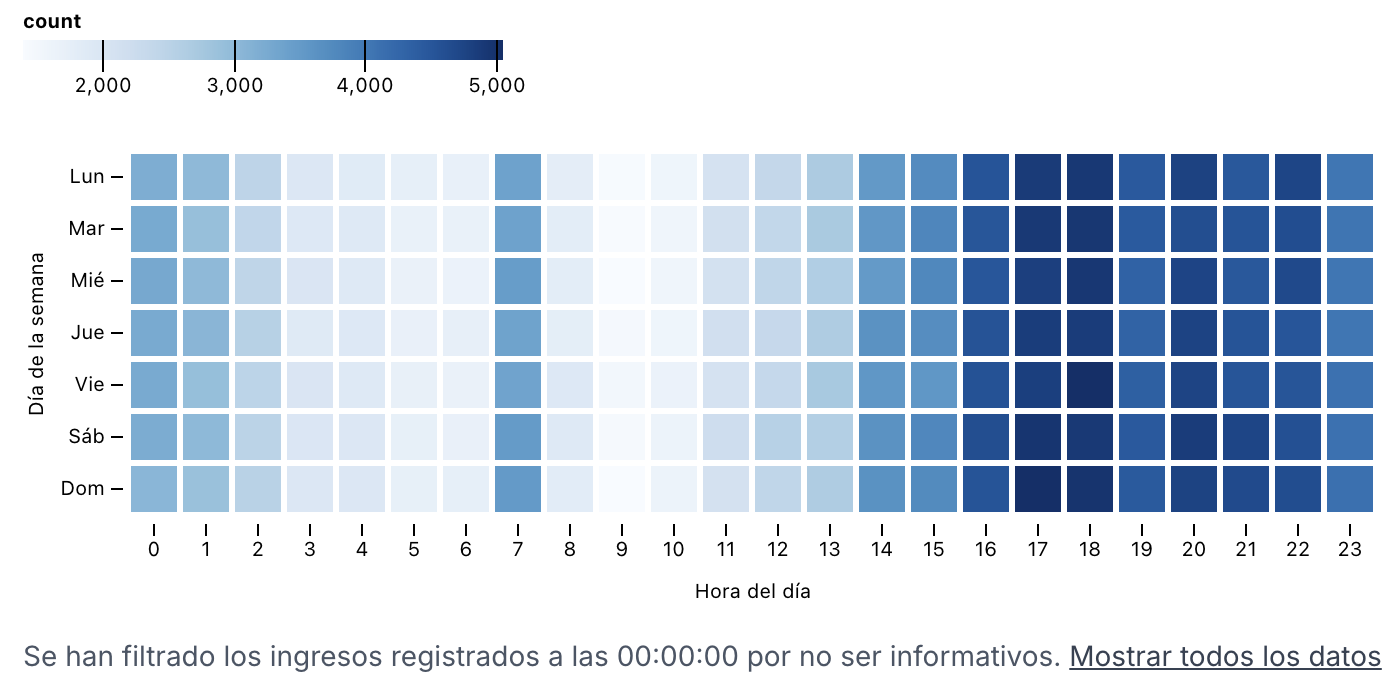
\includegraphics[width=0.8\textwidth]{imagenes/chart-heat-1.png}}
  %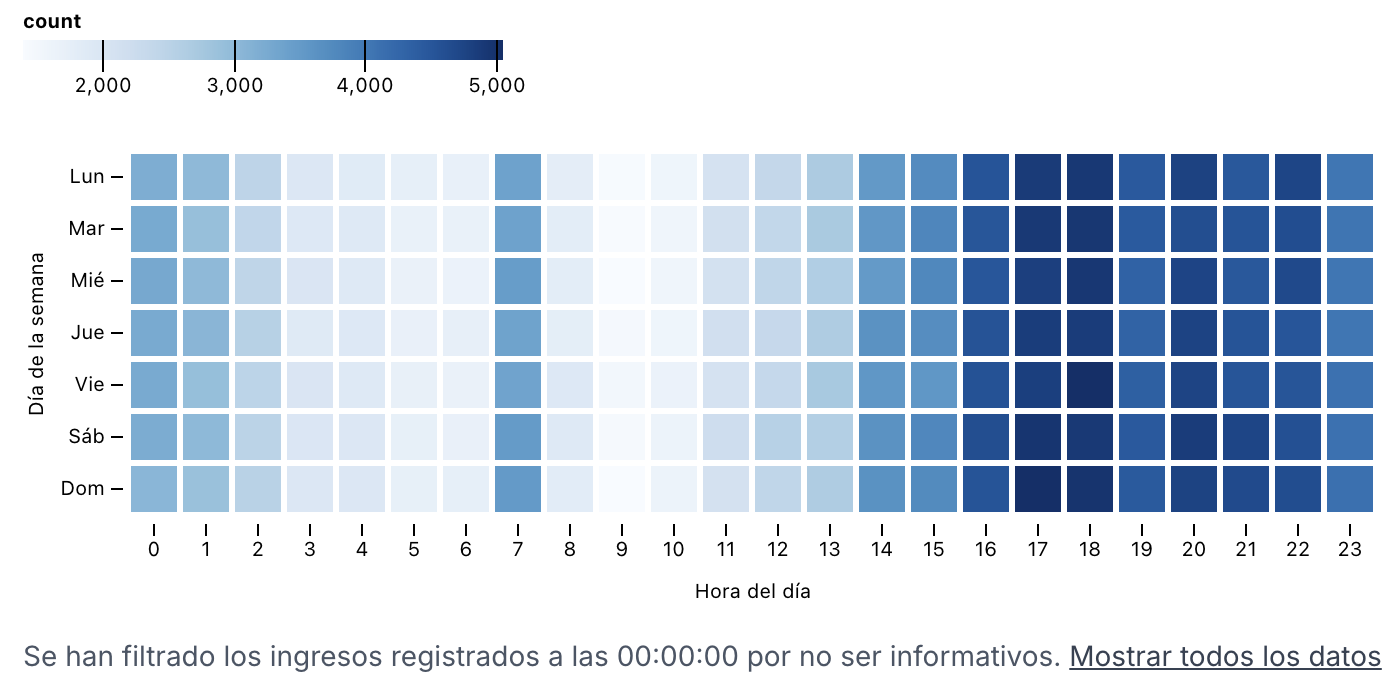
\includegraphics[width=0.8\textwidth]{imagenes/chart-heat-1.png}
  \caption{Heatmap de ingresos por hora y día de la semana.}
  \label{fig:chart-heat-1}
\end{figure}

\begin{figure}[H]
  \centering
  \fbox{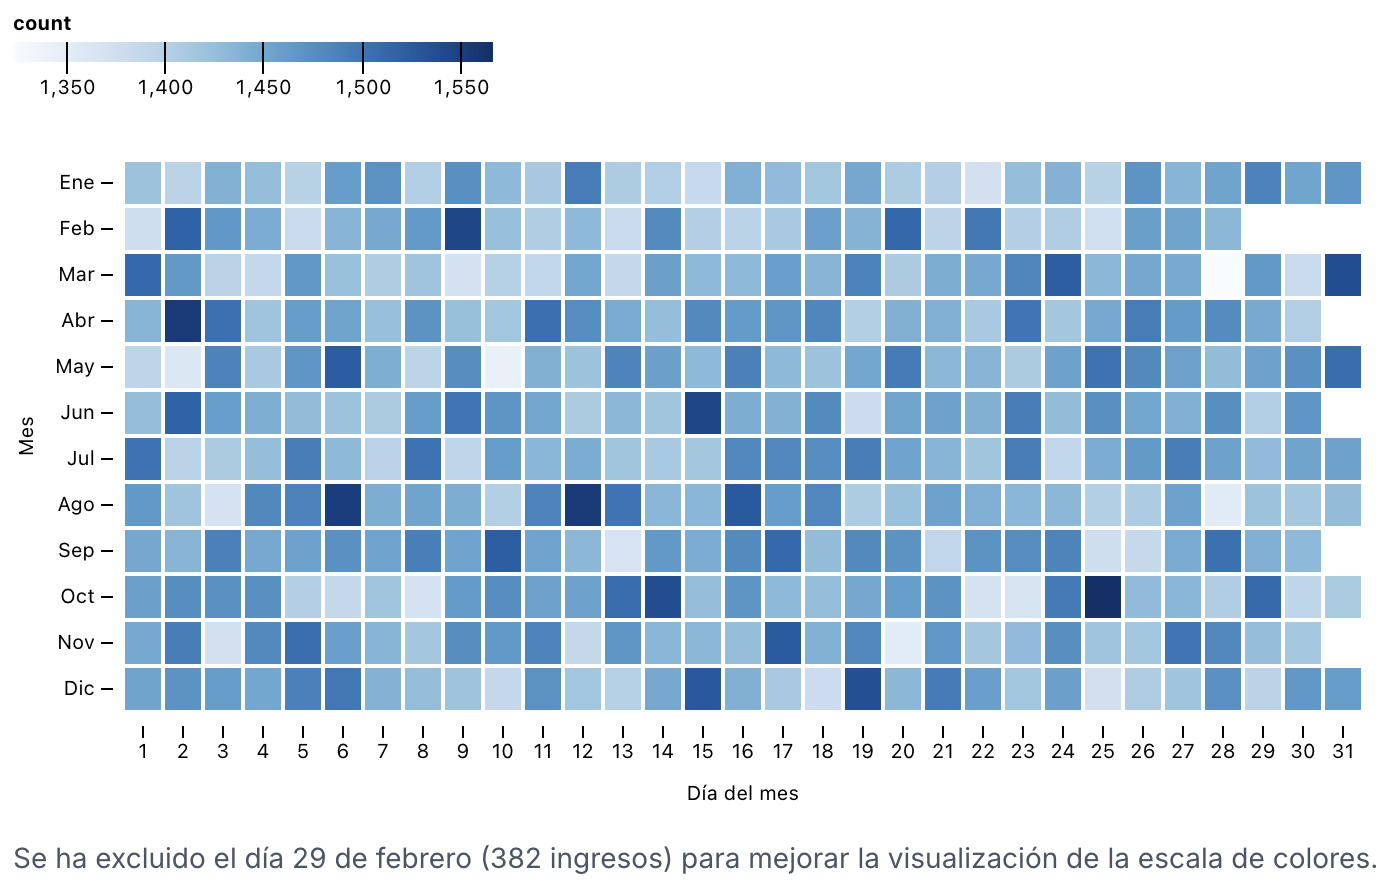
\includegraphics[width=0.8\textwidth]{imagenes/chart-heat-2.png}}
  %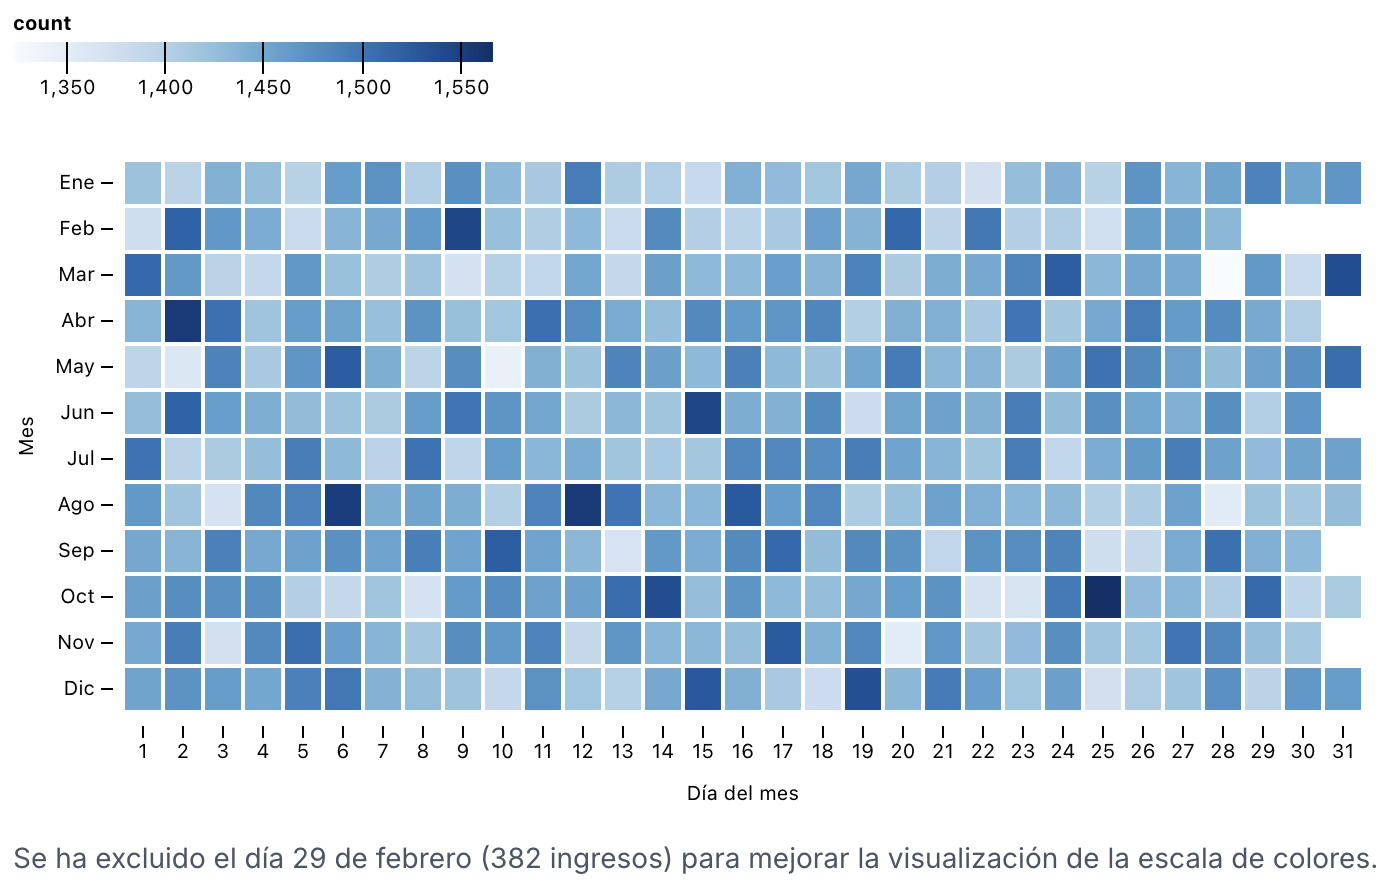
\includegraphics[width=0.8\textwidth]{imagenes/chart-heat-2.png}
  \caption{Heatmap de ingresos por mes y día del mes.}
  \label{fig:chart-heat-2}
\end{figure}


%-----------------
\subsubsection{Página de gráfico: duración de estancias por unidad UCI}

Este gráfico, un Horizontal Bar Chart \cite{hbarchart} de Observable Plot, muestra cual es el  número de días promedio de estancia para cada unidad UCI. Se ha implementado un input para modificar el umbral mínimo de estancias, ya que hay unidades con muy pocas estancias que pueden no ser informativas. Un ejemplo es la unidad \texttt{Neurology}, que sólo tiene una estancia, y es de 28 días, muy por encima del resto. 

%Cabe destacar que pasando el cursor por encima de cada barra, se muestra el numero exacto de estancias para esa unidad.


\begin{figure}[H]
  \centering
  \fbox{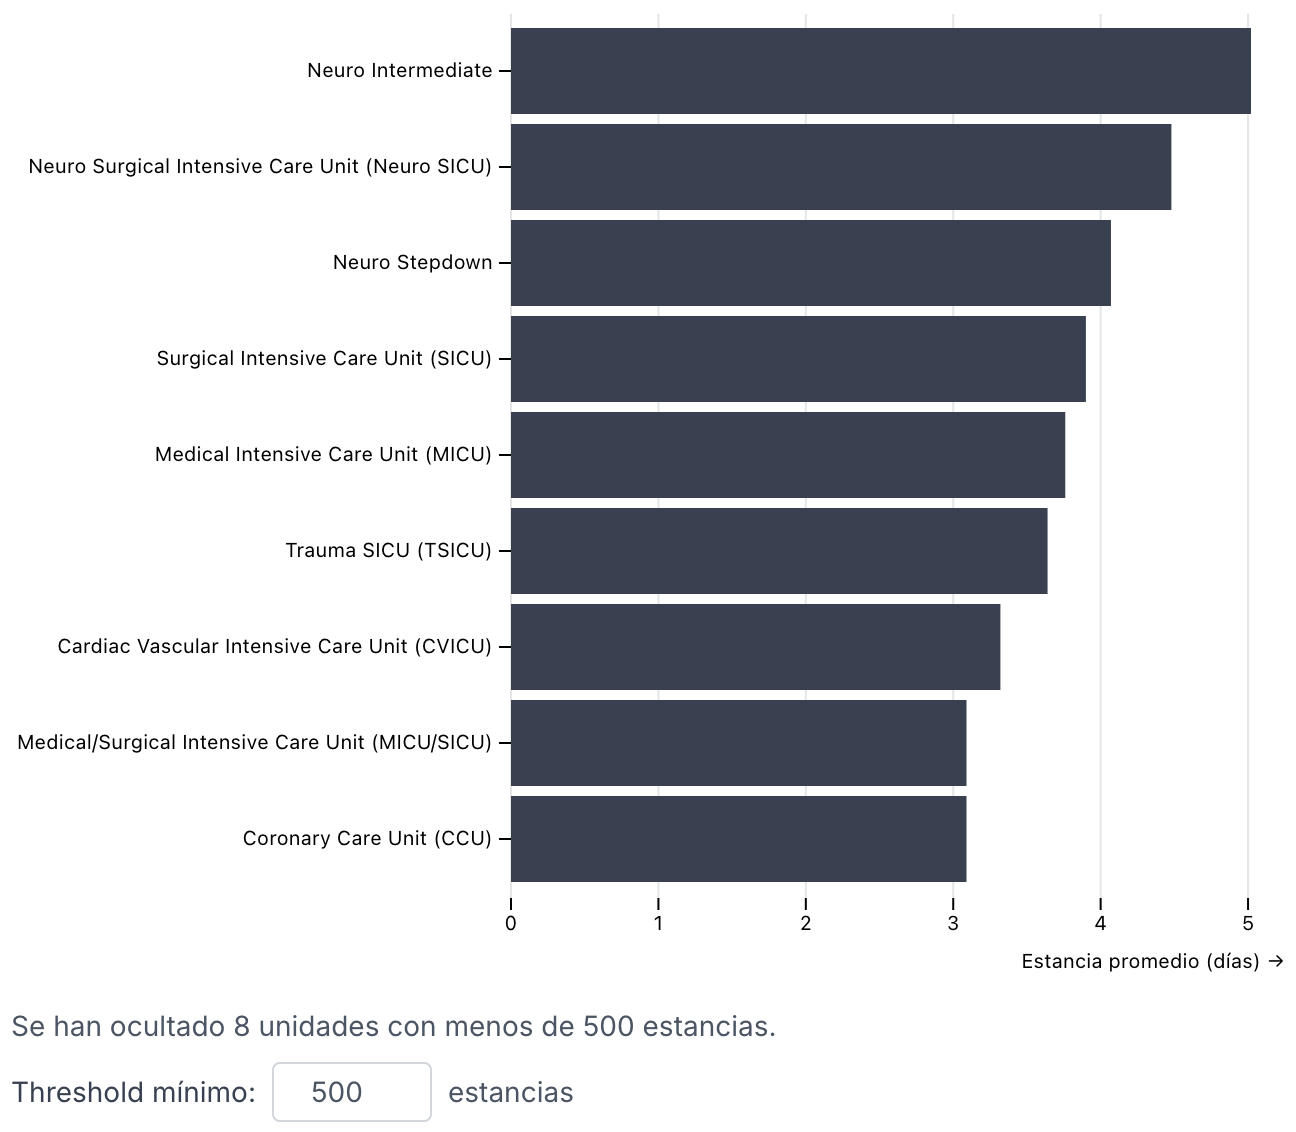
\includegraphics[width=0.75\textwidth]{imagenes/chart-icu.png}}
  %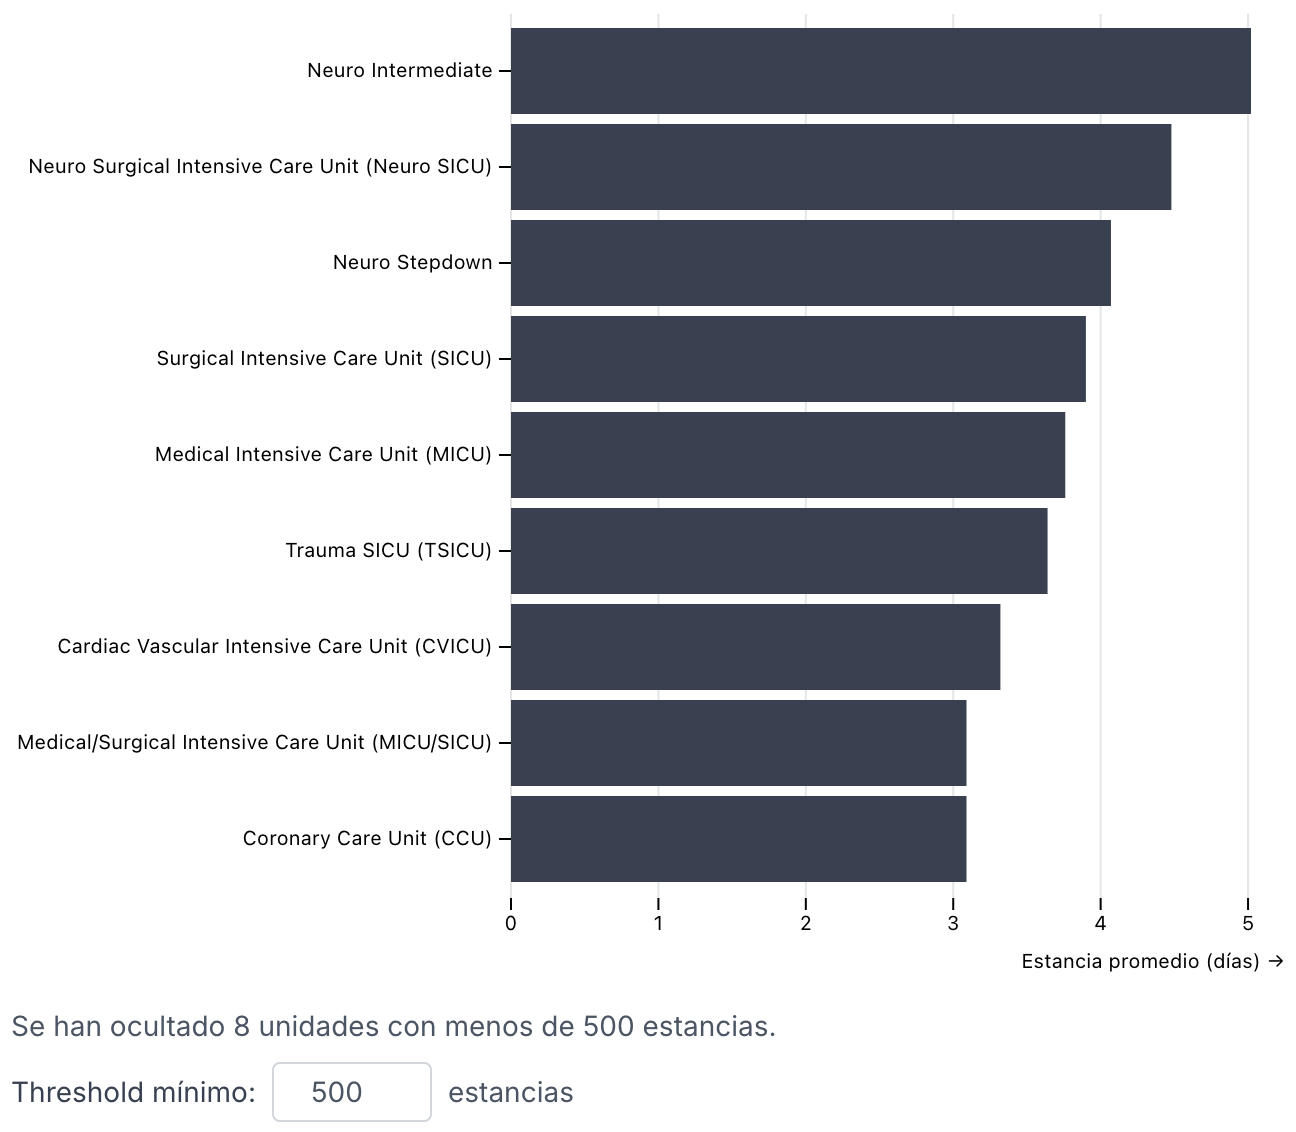
\includegraphics[width=0.75\textwidth]{imagenes/chart-icu.png}
  \caption{Estancia promedio por unidad UCI}
  \label{fig:chart-icu}
\end{figure}


%-----------------
\subsubsection{Página de gráfico: medicamentos más prescritos por vía}

Esta visualización es más compleja que las anteriores, por lo que se hace uso de la librería D3. Se trata de un gráfico Sunburst interactivo \cite{sunburst}, que permite hacer zoom para moverse por la información. Se muestran los medicamentos más prescritos por vía de administración. Para este gráfico, debido a la enorme cantidad de documentos (más de 20 millones) en la colección donde se aloja esta información \texttt{hosp\_prescriptions}, en lugar de obtener los datos en cada llamada al endpoint del backend, se ha realizado una colección nueva mediante un script Python, que contiene los datos ya pre-agregados. De nuevo, debido a la cantidad masiva de datos, se implementan unos filtros de umbral mínimo y máximo para facilitar la visualización.

\begin{figure}[H]
  \centering
  \fbox{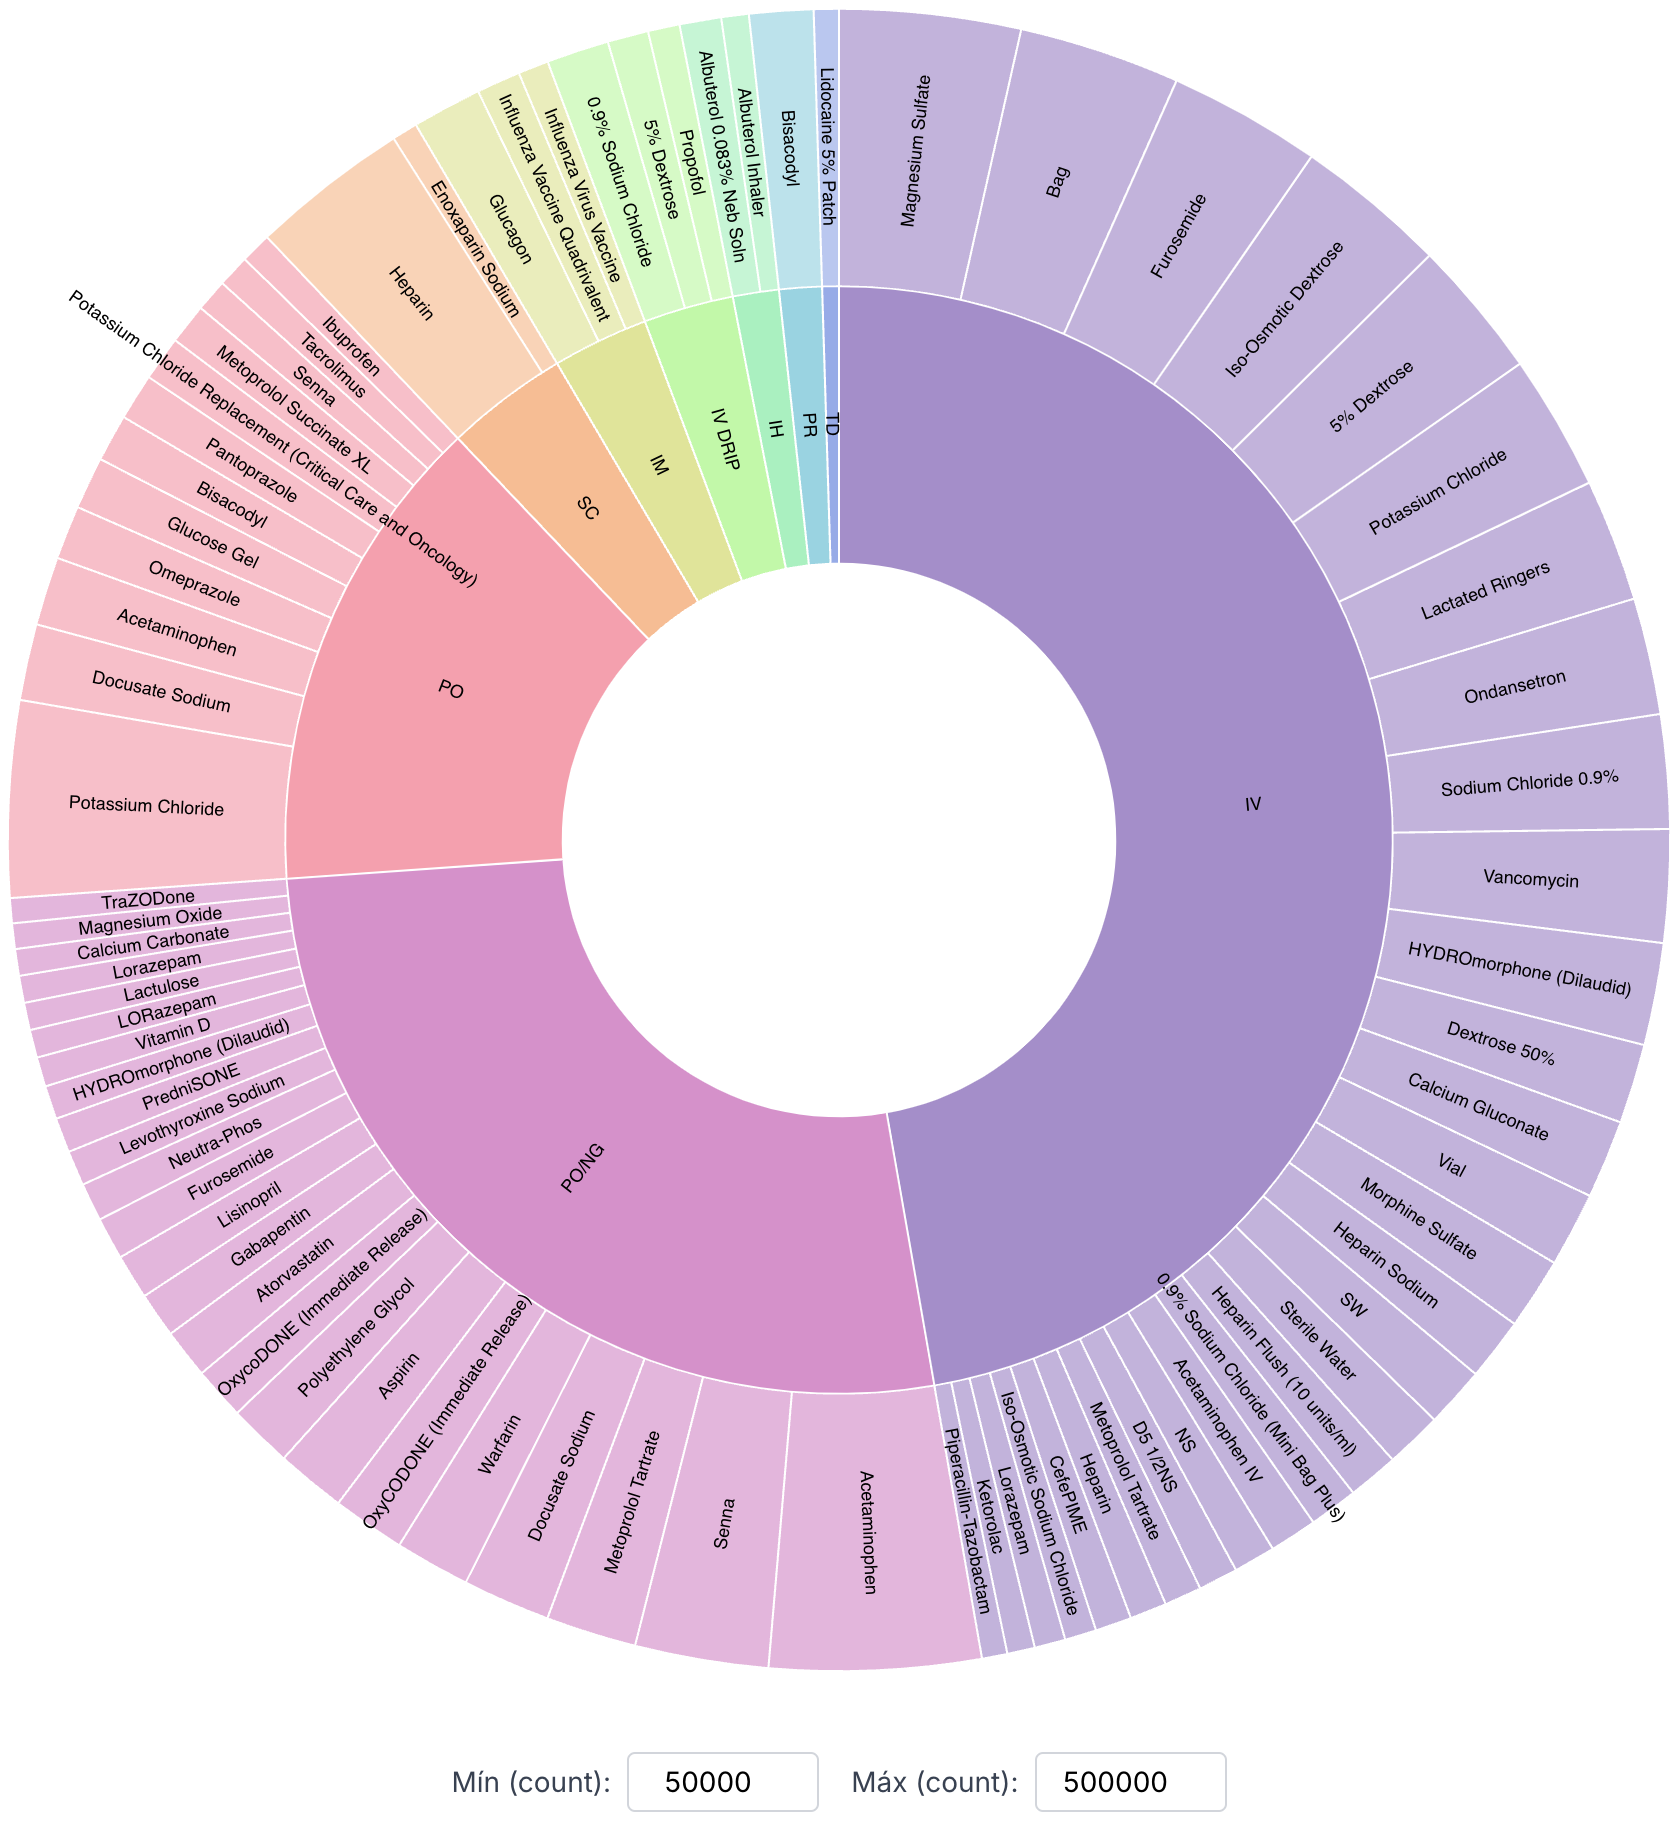
\includegraphics[width=0.85\textwidth]{imagenes/chart-sunburst.png}}
  %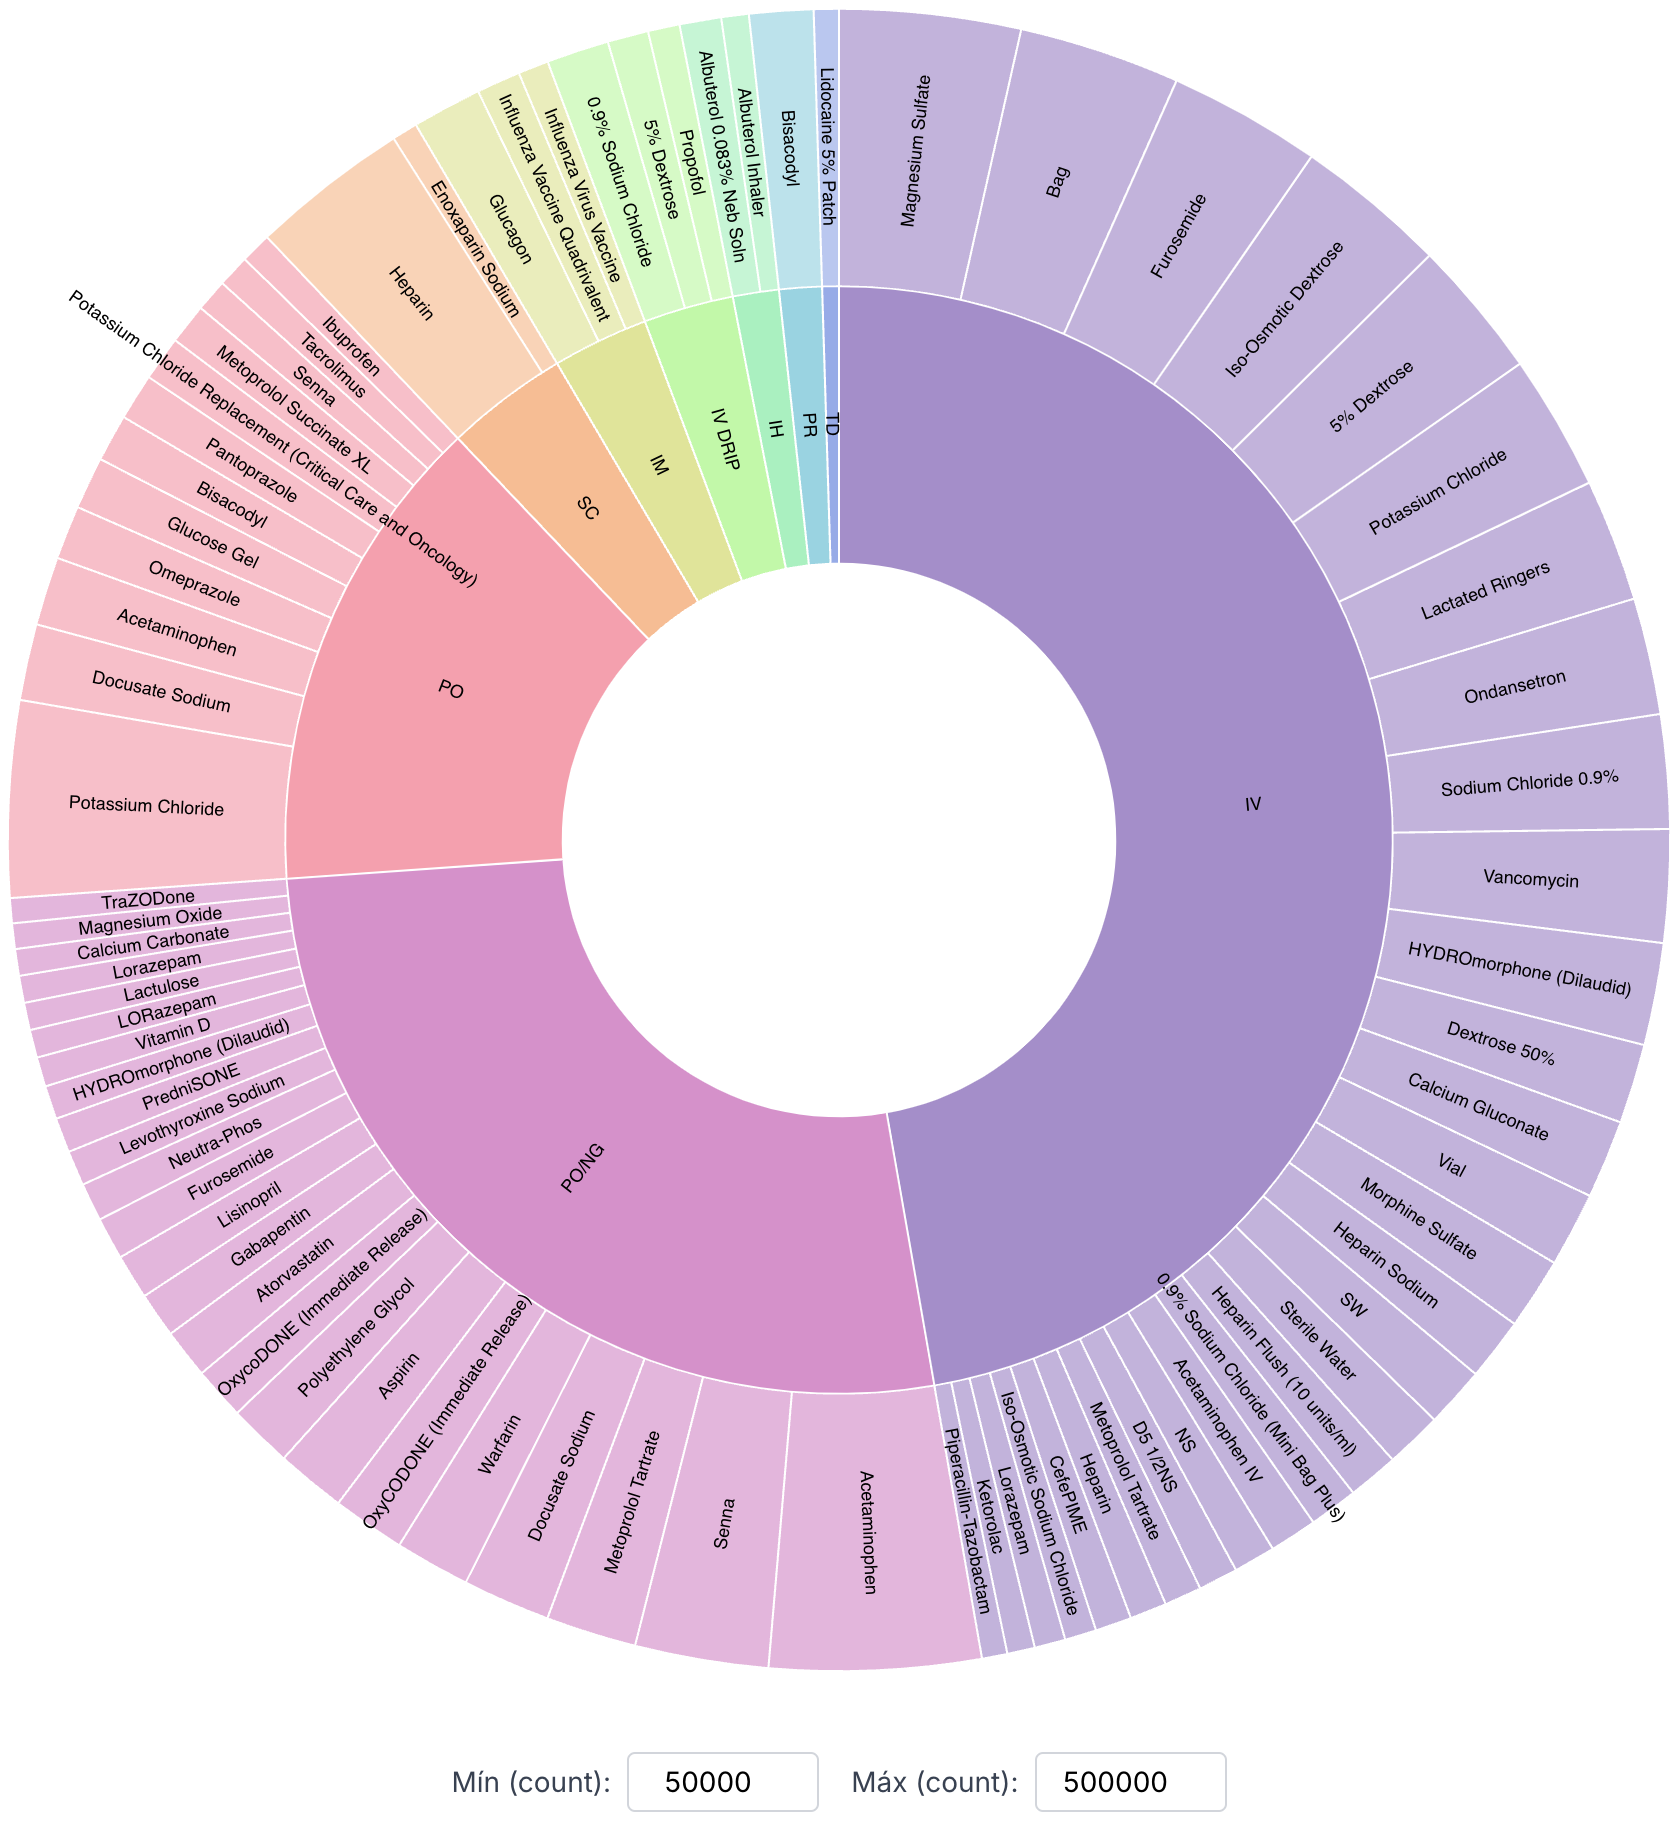
\includegraphics[width=0.85\textwidth]{imagenes/chart-sunburst.png}
  \caption{Medicamentos más prescritos por vía}
  \label{fig:chart-sunburst}
\end{figure}




%-----------------
\subsubsection{Página de gráfico: número de diagnósticos por categorías}




\begin{figure}[H]
  \centering
  \fbox{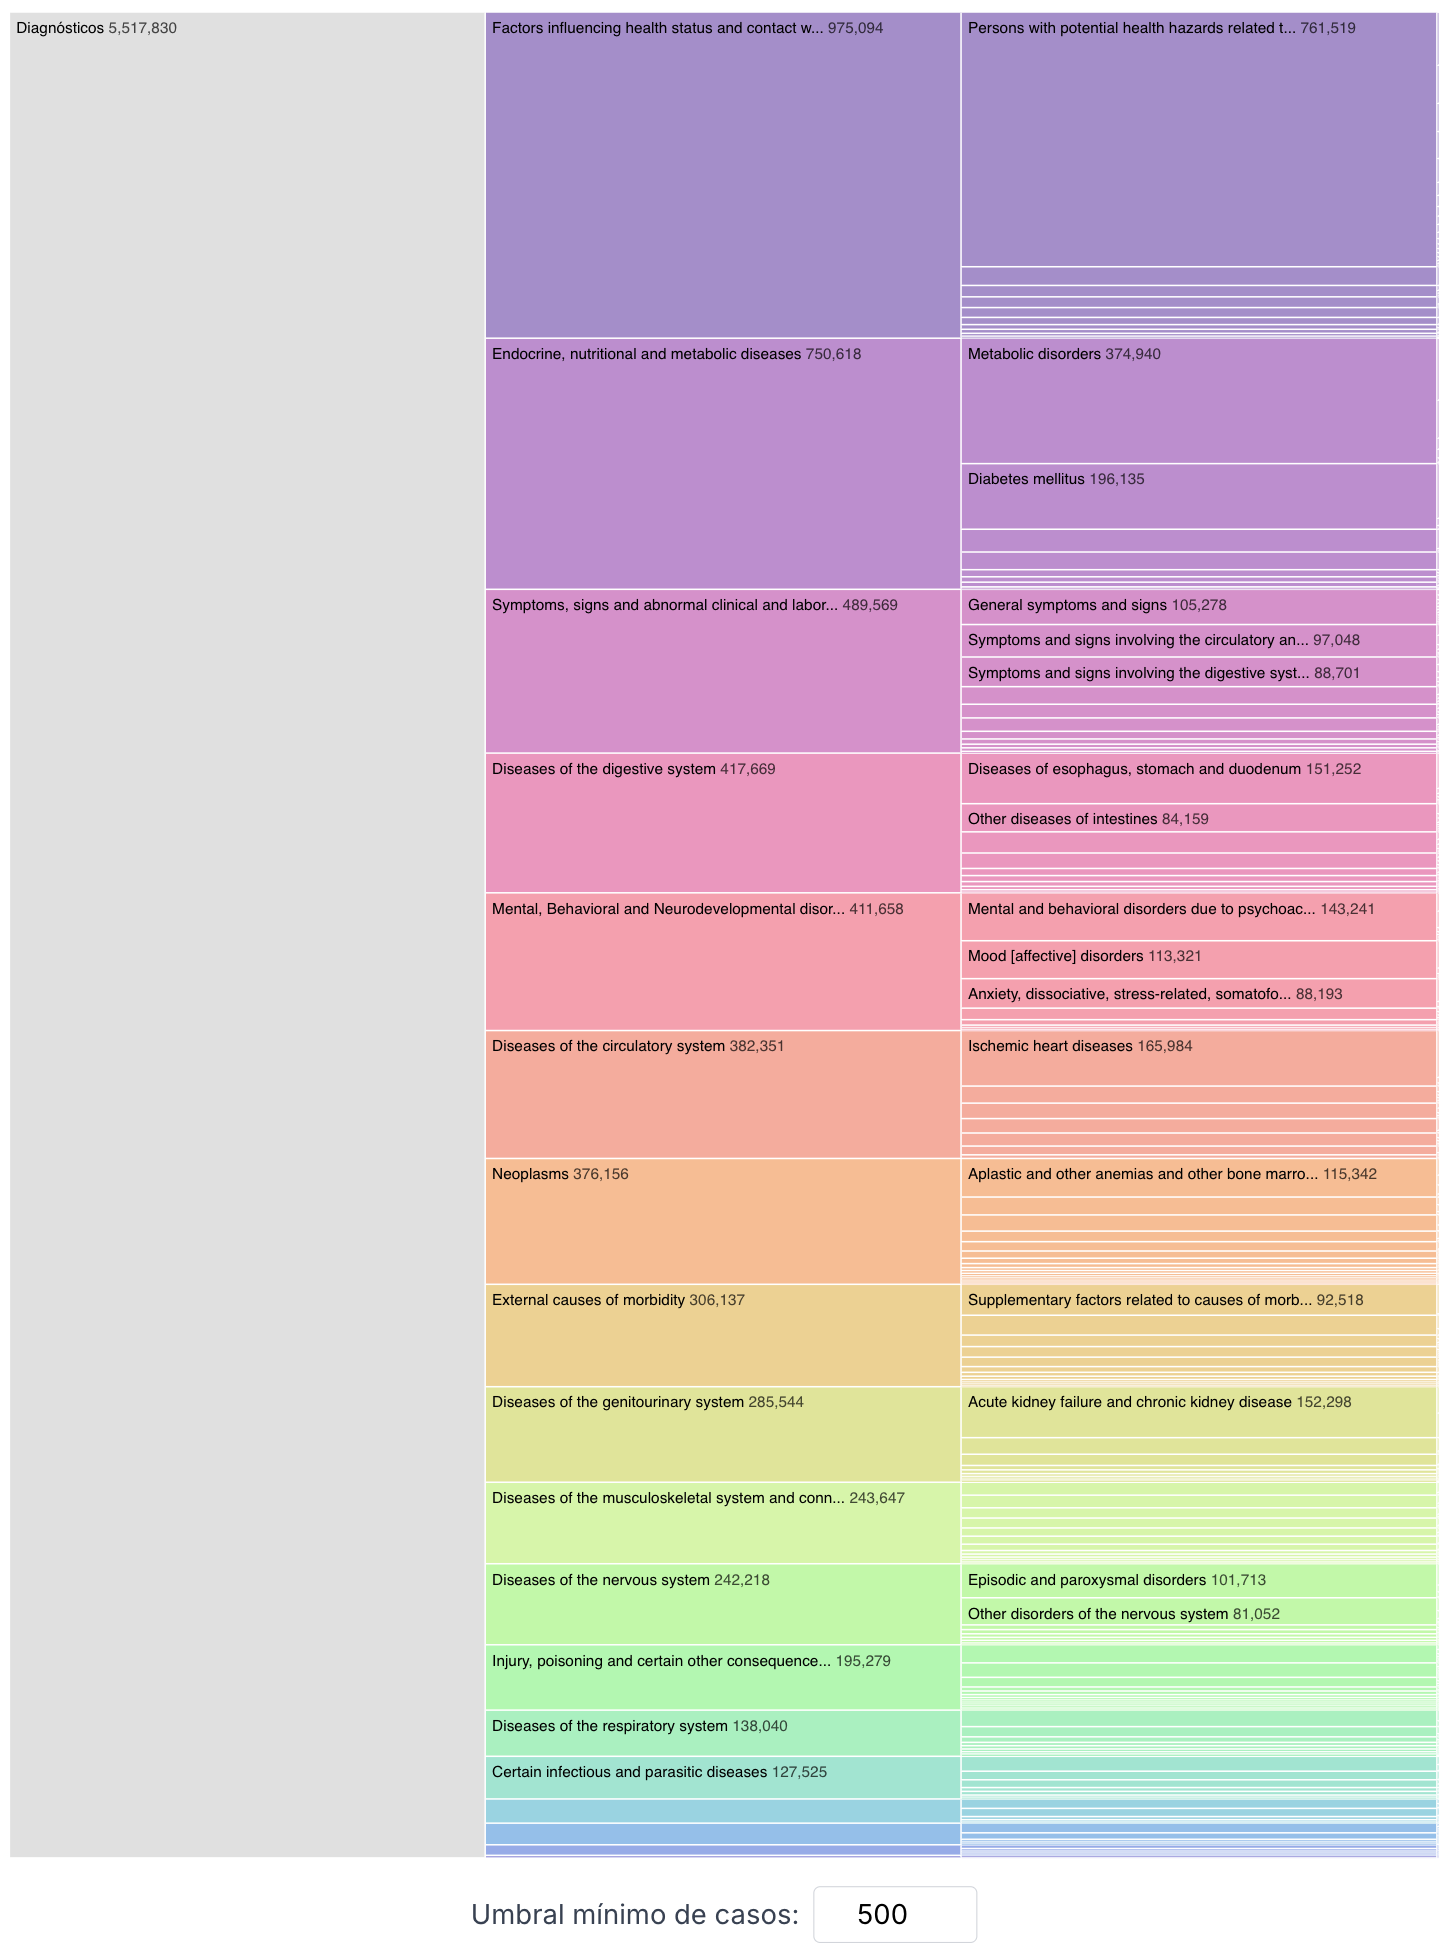
\includegraphics[width=0.88\textwidth]{imagenes/chart-diag.png}}
  %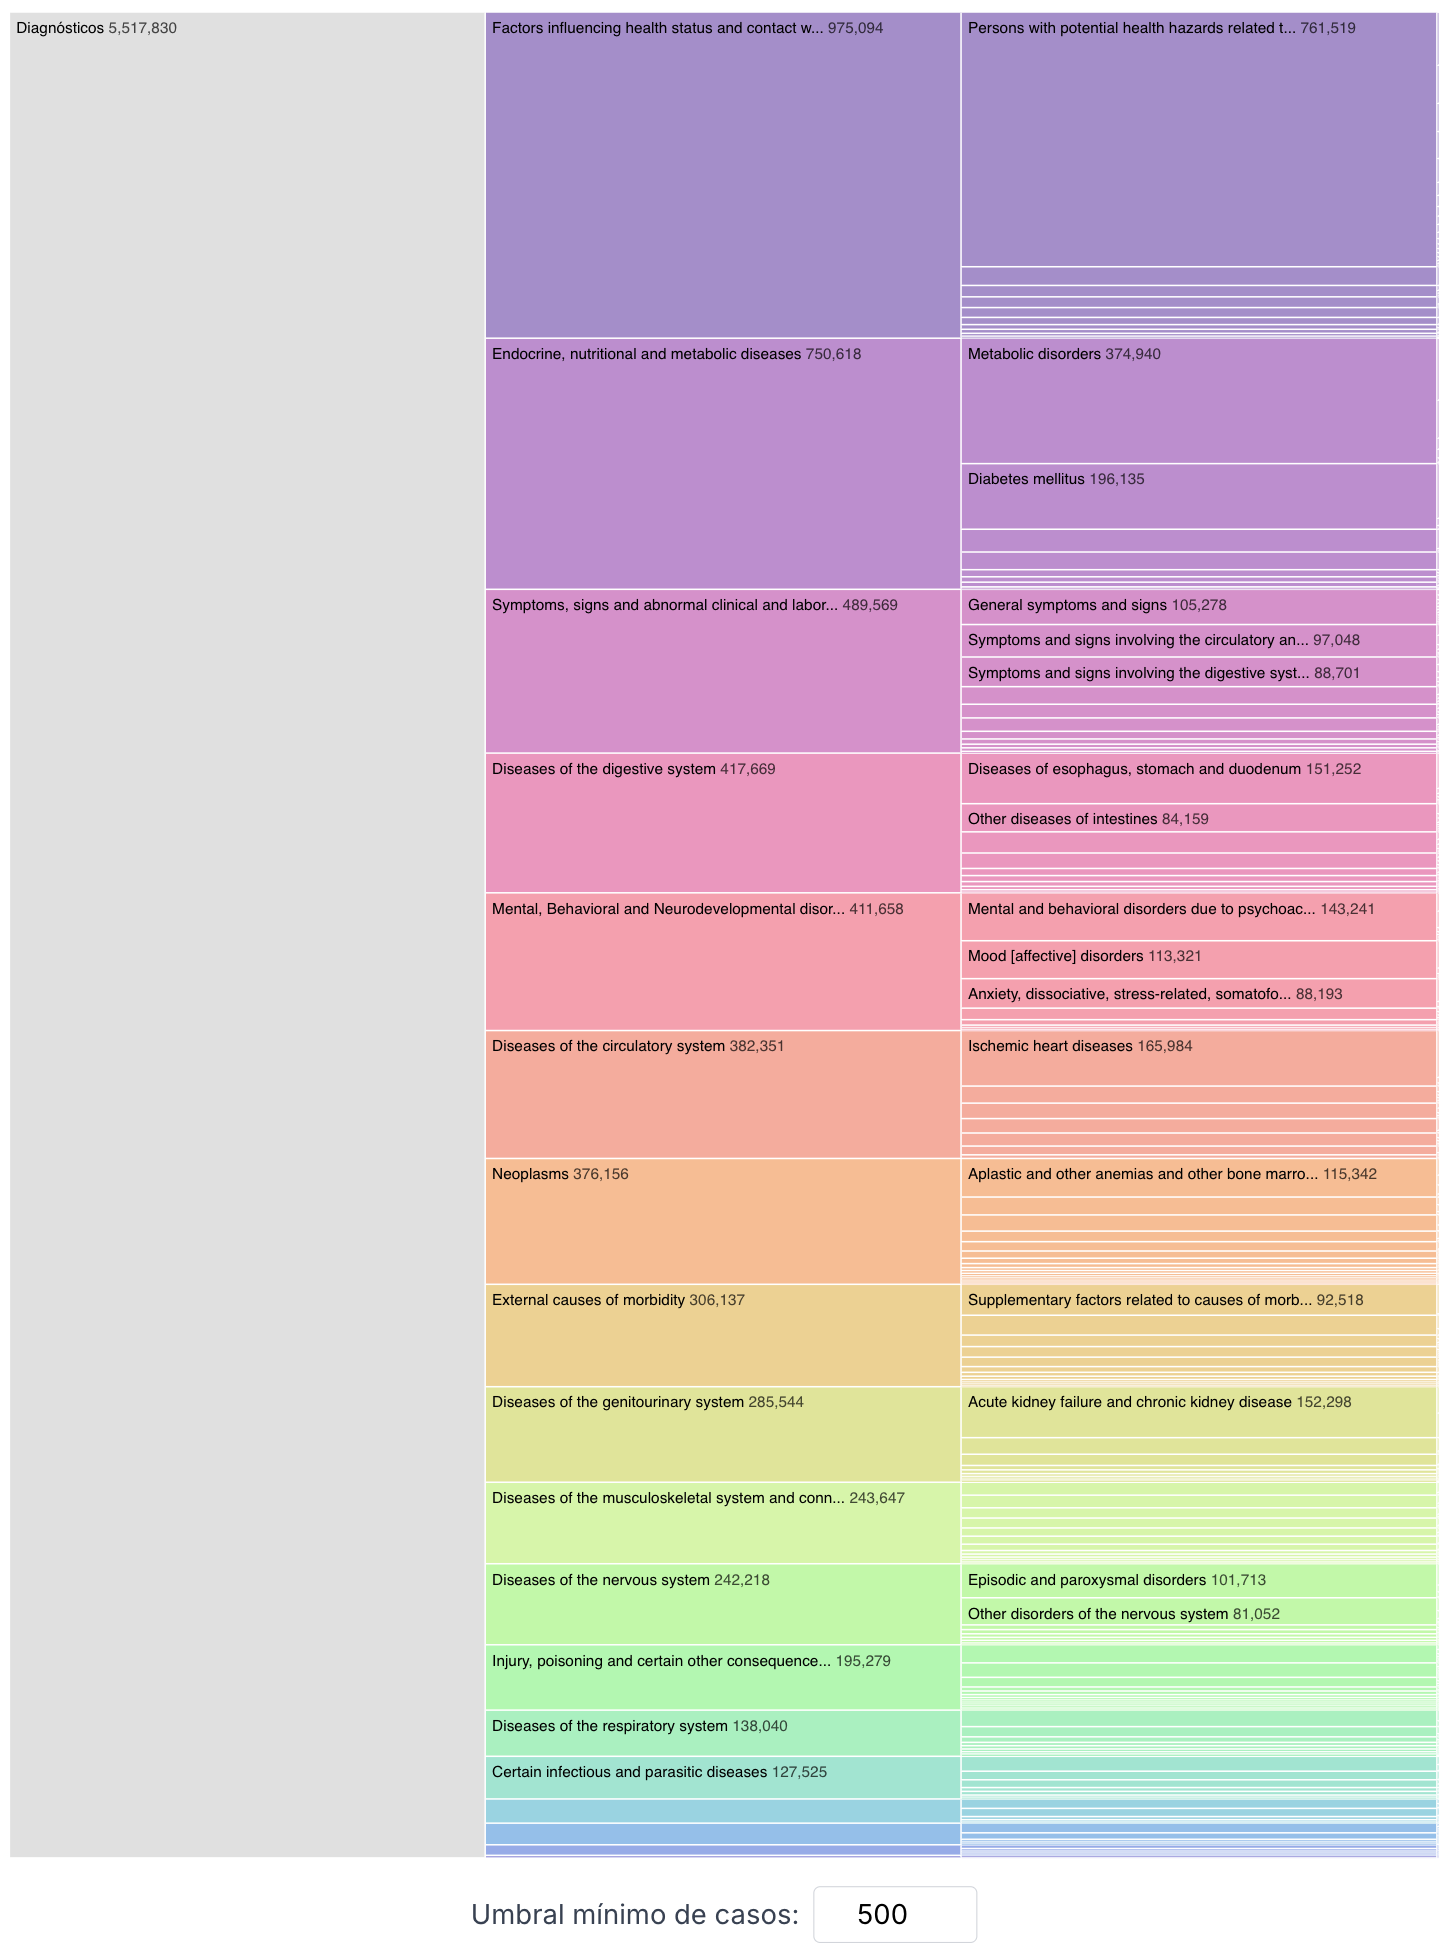
\includegraphics[width=0.88\textwidth]{imagenes/chart-diag.png}
  \caption{Zoomable icicle chart de diagnósticos por categoría}
  \label{fig:chart-diag}
\end{figure}

%habria q poner un ejemplo de como se puede hacer zoom? 


%-----------------
\subsubsection{Página de gráficos: flujos hospitalarios entre unidades}




\begin{figure}[H]
  \centering
  \fbox{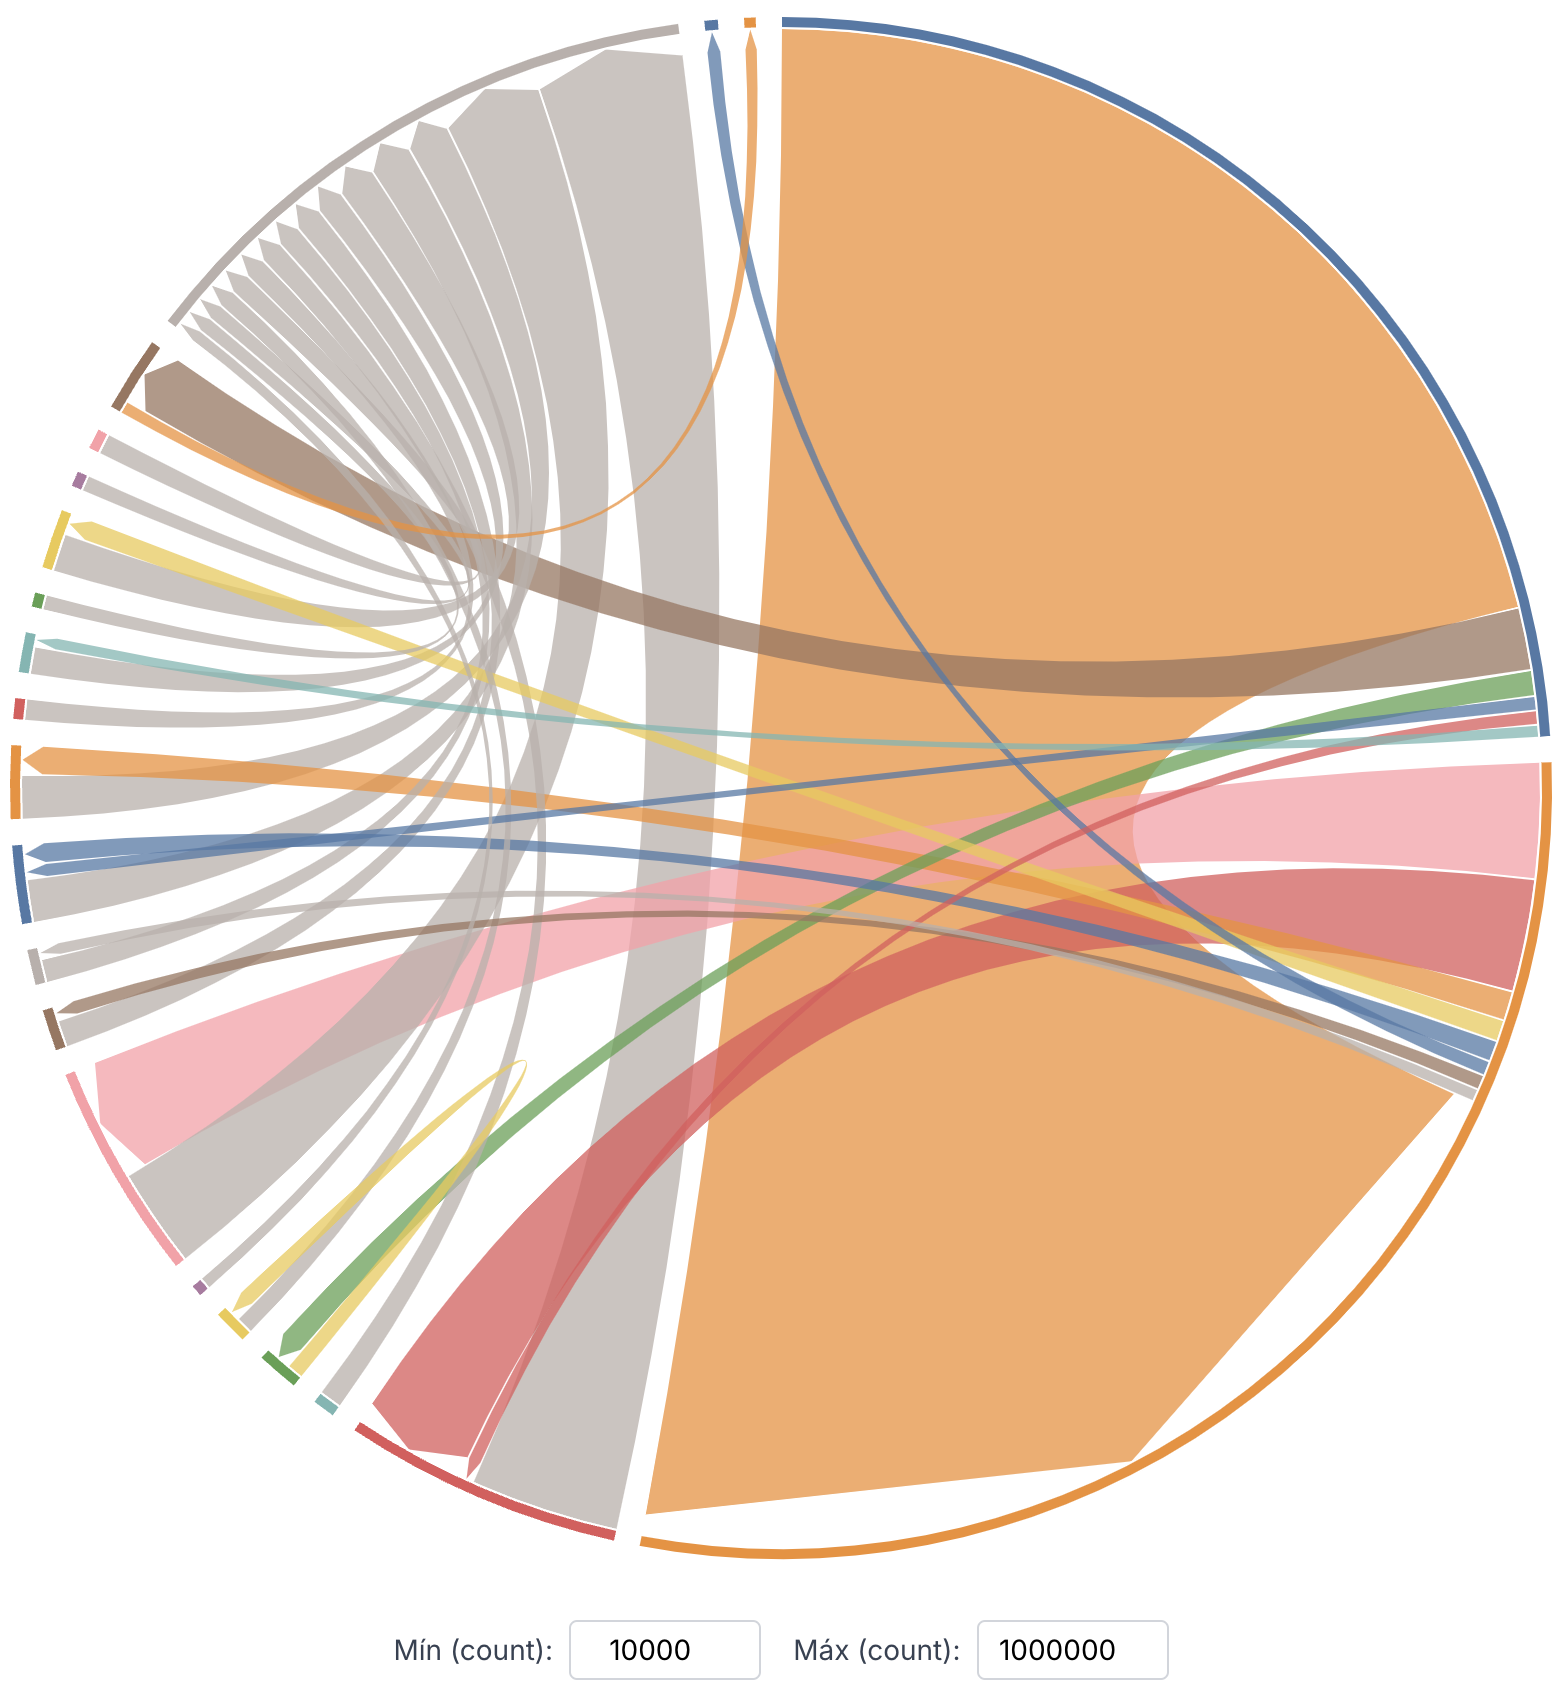
\includegraphics[width=0.88\textwidth]{imagenes/chart-flows.png}}
  %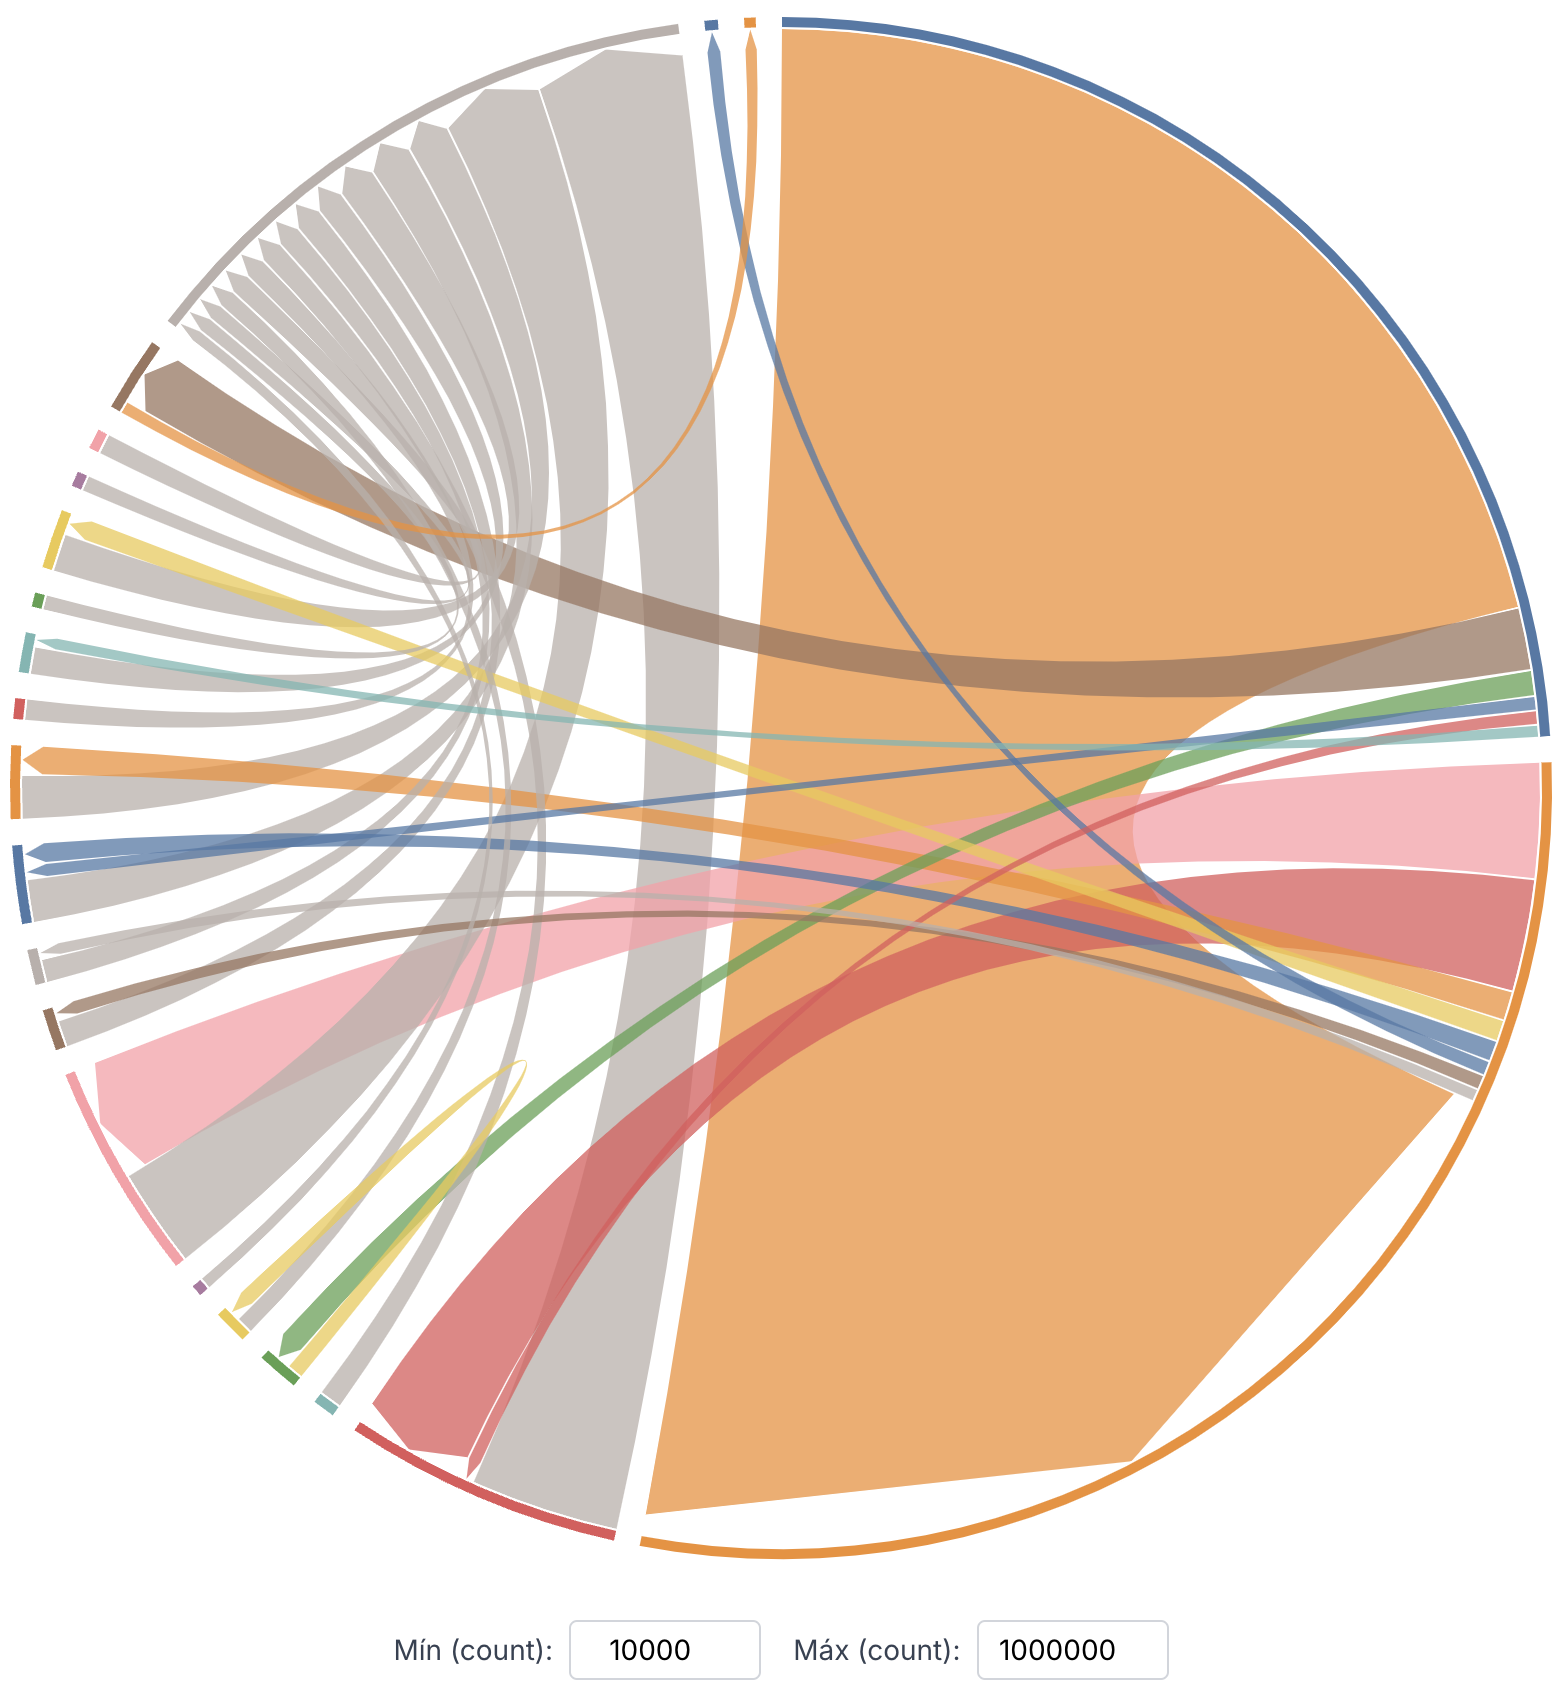
\includegraphics[width=0.88\textwidth]{imagenes/chart-flows.png}
  \caption{Flujos hospitalarios}
  \label{fig:chart-flows}
\end{figure}




@todo: hablar de cada grafico la info que aporta?

@todo: explicar como seria el proceso de agregar un grafico nuevo?

\subsection{Despliegue}

El frontend de la aplicación se ha desplegado utilizando la plataforma Vercel, una solución en la nube especializada en el despliegue de aplicaciones web moderna. LLa elección se fundamenta en varias ventajas clave para este proyecto:

\begin{itemize}
    \item \textbf{Integración nativa con Next.js}: Al ser Vercel la empresa creadora de Next.js, la plataforma ofrece soporte optimizado y características específicas para este framework, incluyendo optimización automática de bundles, Server-Side Rendering (SSR) y Static Site Generation (SSG).
    
    \item \textbf{Red de distribución global (CDN)}: Vercel distribuye automáticamente la aplicación a través de su red global de servidores edge, garantizando tiempos de carga mínimos desde cualquier ubicación geográfica.
    
    \item \textbf{Despliegues instantáneos}: El tiempo de despliegue es típicamente inferior a 30 segundos, permitiendo iteraciones rápidas durante el desarrollo.
    
    \item \textbf{Plan gratuito generoso}: Para proyectos académicos y de desarrollo, Vercel ofrece un tier gratuito que incluye 100GB de bandwidth mensual, despliegues ilimitados y dominio personalizado.
\end{itemize}

\subsubsection{Implementación de CI/CD}

Se ha implementado un pipeline de CI/CD (Continuous Integration/Continuous Deployment) que automatiza completamente el proceso de despliegue. CI/CD es una metodología de desarrollo que automatiza la integración, testing y despliegue de código, permitiendo entregar actualizaciones de software de forma rápida, segura y consistente.

El flujo de trabajo implementado funciona de la siguiente manera:

\begin{enumerate}
    \item \textbf{Detección automática de cambios}: Cada vez que se realiza un push al repositorio principal en GitHub, Vercel detecta automáticamente los cambios mediante webhooks.
    
    \item \textbf{Proceso de construcción}: Vercel ejecuta automáticamente los comandos de build de Next.js (\texttt{npm run build}), optimizando el código para producción, incluyendo tree-shaking, minificación y code-splitting.
    
    \item \textbf{Validación y testing}: Durante el proceso de build, se ejecutan las validaciones de TypeScript y ESLint configuradas en el proyecto.
    
    \item \textbf{Despliegue atómico}: Una vez completada la construcción exitosamente, Vercel despliega la nueva versión de forma atómica, garantizando que no hay tiempo de inactividad.
    
    \item \textbf{Invalidación de caché}: Se invalida automáticamente la caché de CDN para asegurar que los usuarios reciban inmediatamente la nueva versión.
\end{enumerate}

Esta implementación garantiza que la versión en producción refleje siempre el estado actual del código en el repositorio principal, facilita la colaboración en el desarrollo y reduce significativamente el riesgo de errores humanos durante el despliegue. La aplicación frontend está accesible en producción a través de la URL \url{https://tfg.angeloyo.com}.


\begin{figure}[H]
  \centering
  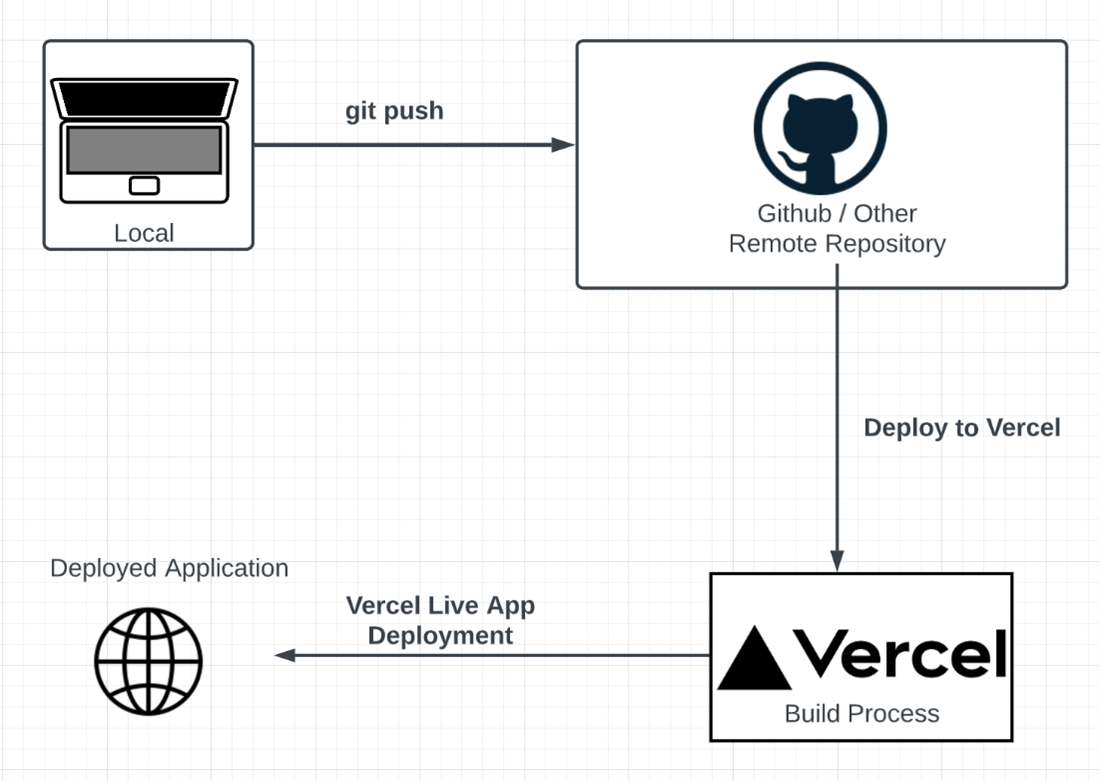
\includegraphics[width=0.8\textwidth]{imagenes/cicd.png}
  \caption{Esquema del depliegue con Vercel \cite{cicdfoto}.}
  \label{fig:cicd}
\end{figure}
